% Copyright (C) 2013 Columbia University in the City of New York and others.
%
% Please see the AUTHORS file in the main source directory for a full list
% of contributors.
%
% This file is part of TerraFERMA.
%
% TerraFERMA is free software: you can redistribute it and/or modify
% it under the terms of the GNU Lesser General Public License as published by
% the Free Software Foundation, either version 3 of the License, or
% (at your option) any later version.
%
% TerraFERMA is distributed in the hope that it will be useful,
% but WITHOUT ANY WARRANTY; without even the implied warranty of
% MERCHANTABILITY or FITNESS FOR A PARTICULAR PURPOSE. See the
% GNU Lesser General Public License for more details.
%
% You should have received a copy of the GNU Lesser General Public License
% along with TerraFERMA. If not, see <http://www.gnu.org/licenses/>.

\documentclass[10pt,twoside,openright]{memoir}
\usepackage[english]{babel}
\usepackage{tgtermes}
\usepackage[colorlinks=true]{hyperref}

\usepackage{mathpazo}
\usepackage[protrusion=true,expansion=true]{microtype}
\usepackage{lettrine}
\usepackage{graphicx}
\usepackage{amsfonts,amsmath,amssymb,amsthm,amsbsy,amssymb,bm}
\usepackage{xcolor}
\usepackage{enumitem}

\usepackage[final]{listings}
\lstloadlanguages{[LaTeX]TeX,Python,bash,[gnu]Make,XML}

\lstset{basicstyle=\footnotesize\ttfamily,
  emph=anyfield,
  emphstyle=\textit,
  morekeywords={pure},
  escapeinside=`'
}

\lstdefinestyle{Bash}{
  language=bash,
  basicstyle=\small\sffamily,
  frame=tb,
  columns=fullflexible,
  backgroundcolor=\color{yellow!20},
  linewidth=0.9\linewidth,
  xleftmargin=0.1\linewidth
}

\lstdefinestyle{UFL}{
  language=Python,
  basicstyle=\small\ttfamily,
  numbers=left,
  numberstyle=\tiny,
  numbersep=3pt,
  frame=tb,
  columns=fullflexible,
  backgroundcolor=\color{yellow!20},
  linewidth=0.9\linewidth,
  xleftmargin=0.1\linewidth
}
\lstdefinestyle{python}{
  language=Python,
  basicstyle=\small\sffamily,
  numbers=left,
  numberstyle=\tiny,
  numbersep=3pt,
  frame=tb,
  columns=fullflexible,
  backgroundcolor=\color{yellow!20},
  linewidth=0.9\linewidth,
  xleftmargin=0.1\linewidth
}
\usepackage{macros}
%\checkandfixthelayout

% See the ``Memoir customise'' template for some common customisations
% Don't forget to read the Memoir manual: memman.pdf

% \title{A Tutorial Cookbook for \TF{}}
% \author{Marc Spiegelman and Cian Wilson\\
% Columbia University/Lamont Doherty Earth Obs.}
% \date{} % Delete this line to display the current date

%% BEGIN TITLE

\makeatletter
\def\maketitle{%
  \null
  \thispagestyle{empty}%
  \vfill
  \begin{center}\leavevmode
    \normalfont
    {\LARGE\raggedleft \@author\par}%
    \hrulefill\par
    {\huge\raggedright \@title\par}%
    %\vskip 1cm
    \vfill
    {\Large \@date\par}%
  \end{center}%
  %\vfill
  \null
  \cleardoublepage
  }
\makeatother
\author{Marc Spiegelman and Cian Wilson}
\title{A Tutorial Cookbook for \TF{}}
\date{\today}


%%% HEADERS & FOOTERS
\pagestyle{ruled} % try also: empty , plain , headings , ruled , Ruled , companion

%%% CHAPTERS
\chapterstyle{demo} % try also: default , section , hangnum , companion , article, demo

%%% Change section number depth
\setsecnumdepth{subsection}
\setcounter{tocdepth}{2}

%%% clean up bib with Siam.bst \sc{} is not supported for some reason
\renewcommand{\sc}{}






%\includeonly{chapter1,chapter2,chapter3}
%\includeonly{chapter4,chapter5}
%%% BEGIN DOCUMENT

\begin{document}
\pagestyle{headings}
\let\cleardoublepage\clearpage
\maketitle
\frontmatter

\null\vfill

\begin{flushleft}
\textit{A Tutorial Cookbook for \TF}\\
\copyright{ Columbia University in the City of New York and others}\\
DOI: 10.6084/m9.figshare.1466786


\bigskip




ALL RIGHTS RESERVED

\null\vfill


\end{flushleft}
\let\cleardoublepage\clearpage

\newpage
\tableofcontents*
\mainmatter
\sloppy
% Copyright (C) 2013 Columbia University in the City of New York and others.
%
% Please see the AUTHORS file in the main source directory for a full list
% of contributors.
%
% This file is part of TerraFERMA.
%
% TerraFERMA is free software: you can redistribute it and/or modify
% it under the terms of the GNU Lesser General Public License as published by
% the Free Software Foundation, either version 3 of the License, or
% (at your option) any later version.
%
% TerraFERMA is distributed in the hope that it will be useful,
% but WITHOUT ANY WARRANTY; without even the implied warranty of
% MERCHANTABILITY or FITNESS FOR A PARTICULAR PURPOSE. See the
% GNU Lesser General Public License for more details.
%
% You should have received a copy of the GNU Lesser General Public License
% along with TerraFERMA. If not, see <http://www.gnu.org/licenses/>.

\chapter{Introduction}

\TF{},  the\emph{Transparent Finite Element Rapid Model Assembler}, is
a software system for the rapid and reproducible construction and exploration of coupled multi-physics models.

TerraFERMA leverages three advanced open-source libraries for
scientific computation that provide high level problem description
(\href{http://fenicsproject.org}{FEniCS}), composable solvers for
coupled multi-physics problems
(\href{https://www.mcs.anl.gov/petsc}{PETSc}) and a science neutral
options handling system
(\href{https://www.imperial.ac.uk/engineering/departments/earth-science/research/research-groups/amcg/software/spud}{SPuD})
that allows the hierarchical management of all model
options. TerraFERMA inherits most of its functionality from the
underlying libraries but adds a layer of control and guidance for
building reusable and reproducible applications.
% A manuscript describing the design and basic functionality of TerraFERMA can be found here.

As most of the language of \TF{} is also inherited from the underlying
libraries it is also well worth looking at the extensive tutorials for
the \href{http://fenicsproject.org/documentation/tutorial}{FEniCS} project which provide an
excellent introduction to both finite elements and UFL (Unified form
language) for describing weak forms.  It is also well worth
understanding the basic PETSc solver objects for nonlinear solvers
(SNES), Linear solvers (KSP) and Preconditioners (PC) as we will use
the same language for describing solver options (although \TF{}
provides some guidance and subsets of options for choosing).

The purpose of these tutorials is to develop hands-on experience with
\TF{} through detailed, step-by-step examples starting with the
simplest problem of Poisson's equation on a unit square to more
complex multi-physics problems such as time-dependent thermal
convection and non-linear magmatic solitary waves.  The key design
principal of \TF{} is that computational models are, at their most
abstract, a \emph{very large} set of scientific and computational
choices and the purpose of \TF{} is to help the user organize, manage
and modify those choices in a manner that is flexible, reproducible
and reusable.

%\pagebreak{}
\section{Getting and installing the \TF{} software}
\label{sec:gett-inst-tf}

\TF{} is available as an open-source code under a LGPL 3.0
license.  It is hosted as a
\href{https://github.com/terraferma/terraferma}{git repository}.
Installation information, scripts for building from source and
considerably more information is available on the
\href{https://terraferma.github.io}{Wiki} page. 


%%% Local Variables: 
%%% mode: latex
%%% TeX-master: "tftutorials"
%%% End: 

% Copyright (C) 2013 Columbia University in the City of New York and others.
%
% Please see the AUTHORS file in the main source directory for a full list
% of contributors.
%
% This file is part of TerraFERMA.
%
% TerraFERMA is free software: you can redistribute it and/or modify
% it under the terms of the GNU Lesser General Public License as published by
% the Free Software Foundation, either version 3 of the License, or
% (at your option) any later version.
%
% TerraFERMA is distributed in the hope that it will be useful,
% but WITHOUT ANY WARRANTY; without even the implied warranty of
% MERCHANTABILITY or FITNESS FOR A PARTICULAR PURPOSE. See the
% GNU Lesser General Public License for more details.
%
% You should have received a copy of the GNU Lesser General Public License
% along with TerraFERMA. If not, see <http://www.gnu.org/licenses/>.

\chapter{Poisson's Equation on the unit square}
\label{cha:poiss-equat-unit}

\section{Problem Overview}
\label{sec:problem-formulation}

A classic problem for learning any new PDE solver package is to
consider  Poisson's equation on the unit square,  with unit
forcing and homogeneous dirichlet boundary conditions.  The strong
form of this problem is
\begin{align}
-\nabla^2u &= f \quad\text{in } \Omega=[0,1]\times[0,1]\\
u &= 0 \quad\text{on } \partial\Omega
\end{align}
with  prescribed function, $f(x)=1$. 

To solve this problem using the Galerkin finite element method we must make a set of
additional choices. First we choose a \emph{mesh} and an \emph{element} such as
piecewise linear triangles, which together form a discrete finite
element function space $\fspace$ with suitable choice of basis
functions $\phi_{i}, i=1,\ldots n$. Any function $u\in\fspace$ is just a
linear combination of the basis functions
\begin{equation}
  \label{eq:6}
  u = \sum_{i=1}^{N} w_{i}\phi_{i}
\end{equation}
where $w_{i}$ are a set of weights that map to a discrete vector $\vec{w}$ in $\Rn$.

Next we transform the problem into its weak form by multiplying by a
test function $u_{t}$ and integrating by parts to yield the
variational problem: 
\begin{quote}
  \fbox{\parbox{.9\textwidth}{Find $u\in \fspace$ such that
  \begin{equation}
    \int_\Omega \nabla u_t\cdot \nabla u dx= \int_\Omega u_t f dx.\label{eq:weakpoisson}
  \end{equation}
  for all $u_{t} \in\fspace$.}}
\end{quote}
It is often convenient to rewrite Eq. (\ref{eq:weakpoisson}) in the
notation of linear forms as
\begin{equation}
\label{eq:linearforms}
  a(u,u_{t}) = L(u_{t})
\end{equation}
where
\begin{align}
  \label{eq:5}
  a(u,u_{t}) &= \int_\Omega \nabla u_t\cdot \nabla u dx\\
  L(u_{t})    &=  \int_\Omega u_t f dx
\end{align}
are \emph{bilinear} and \emph{linear} forms respectively.

For a linear problem, Eq. (\ref{eq:weakpoisson}) or (\ref{eq:linearforms})
assembles into the discrete linear algebra problem
\begin{equation}
  \label{eq:1}
  A\vec{w} = \vec{b}
\end{equation}
where $A$ is a matrix, $\vec{w}$ is a vector of values at the degrees
of freedom of the function space and $\vec{b}$ is a vector that is essentially the
projection of the forcing function $f$ onto $\fspace$.  We then need
to choose appropriate solvers for the linear system.

\subsection{Poisson as a non-linear problem}
\label{sec:poisson-as-non}

We could construct a model in \TF{} for this linear problem, however, as many
problems we wish to explore  quickly become non-linear, it is worth
first rephrasing this problem as a non-linear problem, and solve it
using Newton's method.  Newton can always be used for linear problems
and is guaranteed to reach a solution in exactly one iteration. % show this?

The principal idea is to rewrite our initial equation in terms of the residual
\begin{equation}
  \label{eq:2}
  r(u) = -\nabla^2 u - f
\end{equation}
which is zero, if $u$ is a solution.  The variational form of this
problem  is then:
\begin{quote}
  \fbox{\parbox{.9\textwidth}{Find $u\in\fspace$ such that
\begin{equation}
  \label{eq:3}
  F(u;u_{t}) = \int_{\Omega} u_{t}r\, dx = 0
\end{equation}
for all test functions $u_t\in\fspace$. }}
\end{quote} 
$F(u;u_{t})$ is the weak form of the (possibly non-linear) residual
and is a linear form that assembles into a vector.

For the specific case of Poisson's equation with dirichlet boundary conditions,
the weak form of the residual can be written, after integration by
parts as
\begin{equation}
  \label{eq:4}
  F(u_{i};u_{t}) = \int_{\Omega}
  \left(
    \grad u_{t}\cdot\grad u_{i} - u_{t}f
  \right)dx
\end{equation}
where $u_{i}$ is an arbitrary function in $\fspace$.   Again, if
$u_{i}$ is a solution of the weak (or strong) form of the equations
then $F(u_{i};u_{t})=0$.  However, if  $u_{i}$ is an arbitrary
function, $F(u_{i},u_{t})$ assembles into a vector $\vec{F}$ of the
discrete residual such that $||\vec{F}||>0$.  

Our goal is to iterate on $u_{i}$\footnote{thus the subscript
$i$} until $||\vec{F}||<\mathrm{tol}$ for some norm on $||\vec{F}||$ and stopping
criterion $\mathrm{tol}$.

\subsubsection{Newton's method}
\label{sec:newtons-method}

The general idea is that given some initial guess $u_{i}$ such that
$F(u_{i}; u_{t}) \neq 0$ there is some correction $\delta u_{i}$ such
that
\begin{equation}
  \label{eq:8}
  F(u_{i} + \delta u_{i}; u_{t}) = 0
\end{equation}
Newton's method assumes we can linearize this equation such that
\begin{equation}
  \label{eq:9}
   F(u_{i} + \delta u_{i}; u_{t}) \approx F(u_{i};u_{t}) +
   J(u_{i},\delta u_{i}; u_{t})
\end{equation}
where 
\begin{equation}
  \label{eq:10}
  J(u_{i},\delta u_{i}; u_{t}) = \lim_{\epsilon\rightarrow 0}
  \frac{F(u_{i}+\epsilon\delta u_{i};u_{t}) - F(u_{i};u_{t})}{\epsilon}
\end{equation}
is the functional (Gateaux) derivative of $F$ with respect to
$u_{i}$.  After a bit of algebra, we can see that for this problem
\begin{equation}
  \label{eq:11}
  J(u_{i},\delta u_{i}; u_{t}) = \int_{\Omega} \left(
    \grad u_{t}\cdot\grad \delta u_{i} \right)dx
\end{equation}
which is a bilinear form that is equivalent to $a(\delta u_{i},u_{t})$
(Eq.\ \ref{eq:5}), which assembles into a matrix $\mat{J}$. Combining Eqs.\
(\ref{eq:8}) -- (\ref{eq:10}), Newton's method
states
\begin{quote}
  \fbox{\parbox{.9\textwidth}{while $||\vec{F}||> tol$, solve
\begin{align}
  \label{eq:12}
  J(u_{i},\delta u_{i}; u_{t}) = -F(u_{i};u_{t})
\end{align}
for $\delta u_{i}$ and update
\begin{displaymath}
u_{i+1} = u_{i} + \delta u_{i}.
\end{displaymath}}}
\end{quote}
For the purposes of the rest of this tutorial we will refer to
$F(u_{i};u_{t})$ as the ``weak form of the residual'' and
$J(u_{i},\delta u_{i};u_{t})$ as the ``weak form of the
Jacobian''.  When assembled, Eq. (\ref{eq:12}) is equivalent to the
linear algebra problem $\mat{J}\vec{\delta u} = -\vec{F}$.

\subsubsection{Writing the problem in ufl}
\label{sec:writing-problem-ufl}

The FEniCS project provides a  high level language (UFL) for describing
variational forms and finite elements that allows us to very succinctly write the
non-linear problem  as 
\begin{lstlisting}[style=UFL]
u_e = FiniteElement("Lagrange", triangle, 1)

u_i = Coefficient(u_e)
f   = Coefficient(u_e)
u_t = TestFunction(u_e)
u_a = TrialFunction(u_e)

F   = (inner(grad(u_t), grad(u_i)) - u_t*f)*dx
J   = inner(grad(u_t), grad(u_a))*dx
\end{lstlisting}
The subscripts \texttt{\_i,\_t,\_a} etc. are somewhat non-standard but
are used consistently in \TF{} to describe ufl symbols for the
\emph{iterated function}, \emph{test function}, and \emph{trial
  function}\footnote{the a is for ansatz\ldots{}} respectively.  Here we have
calculated the weak form of the Jacobian analytically. A very useful
feature of UFL, however is that it can also perform automatic
differentiation of forms and the equivalent UFL would be produced
using
\begin{lstlisting}[style=UFL]
J = derivative(F,u_i,u_a)
\end{lstlisting}
where in both descriptions, \texttt{u\_a} is the ufl symbol for the
correction $\delta u_{i}$.  

Given a description of the weak forms in ufl,  FEniCS provides the
Fenics Form Compiler (FFC), which transforms high level UFL into
compileable C++ code using the UFC library for describing assembly of
local tensors over cells etc.  However, UFL and FFC are not sufficient
to describe the full set of choices required to construct a finite
element solution.  In FEniCS,  the \emph{dolfin} library (and its
python interface) provides the integration tools however, one must
construct individual applications from scratch as either python or C++
programs.  The whole purpose of \TF{} is to provide another layer of
integration that assembles the full model application from a
hierarchical options file. 

\section{Solution using \TF}
\label{sec:ch2-solution-using-tf}

To summarize,  the key choices required to fully describe and solve a
basic finite element problem using Newton's method are
\begin{enumerate}
\setlength{\itemsep}{0cm}
\item Choose a mesh
\item Choose Fields to solve $u$
\item Choose an element (Function Space)
\item Choose Initial/Boundary Conditions
\item Choose a weak form for the non-linear residual $F(u)$
\item Calculate the weak form of the Jacobian $J=F'(u)$
\item Choose a method for solving the linear problem $\mat{J}\vec{\delta u} = -\vec{F}$
\item Choose all the other adjustable parameters for controlling and
  monitoring convergence, visualization, output etc.
\end{enumerate}

The design of \TF{} is to use the SPuD library to provide a schema and interface
for managing, recording and documenting all of these choices in an
intuitive options file, from which a compiled C++ application can
be built and run.  These options files have the suffix \texttt{.tfml}
and describe the \emph{\TF{} markup language}\footnote{which is a
  flavor of  xml which should rarely  be read by humans}.  SPuD also provides the gui
\texttt{diamond} that reads and writes \texttt{tfml} files through an
intuitive interface.  

A fully worked out description of Poisson's Equation on the unit
square with unit forcing can be found in the tutorials folder of the
installed software (by default
\texttt{\${TF\_HOME}/share/terraferma/tutorials}) in
\texttt{poisson/simple/poisson.tfml}.  To view this file, simply go to
the source folder and type
\begin{lstlisting}[style=Bash]
$ diamond poisson.tfml
\end{lstlisting}

To build and run the code:
\begin{lstlisting}[style=Bash]
$ tfbuild poisson.tfml
$ cd build
$ make run 
\end{lstlisting}
which will create a build directory \texttt{build} using
\texttt{cmake} then compile and run the code. Output from the run
includes stdout (in \texttt{terraferma.log-0)}, statistics files (see
below) and \texttt{vtk} files that can be visualized using paraview
(or any other vtk visualization system) to produce something like
\begin{figure}[h]
  \centering
  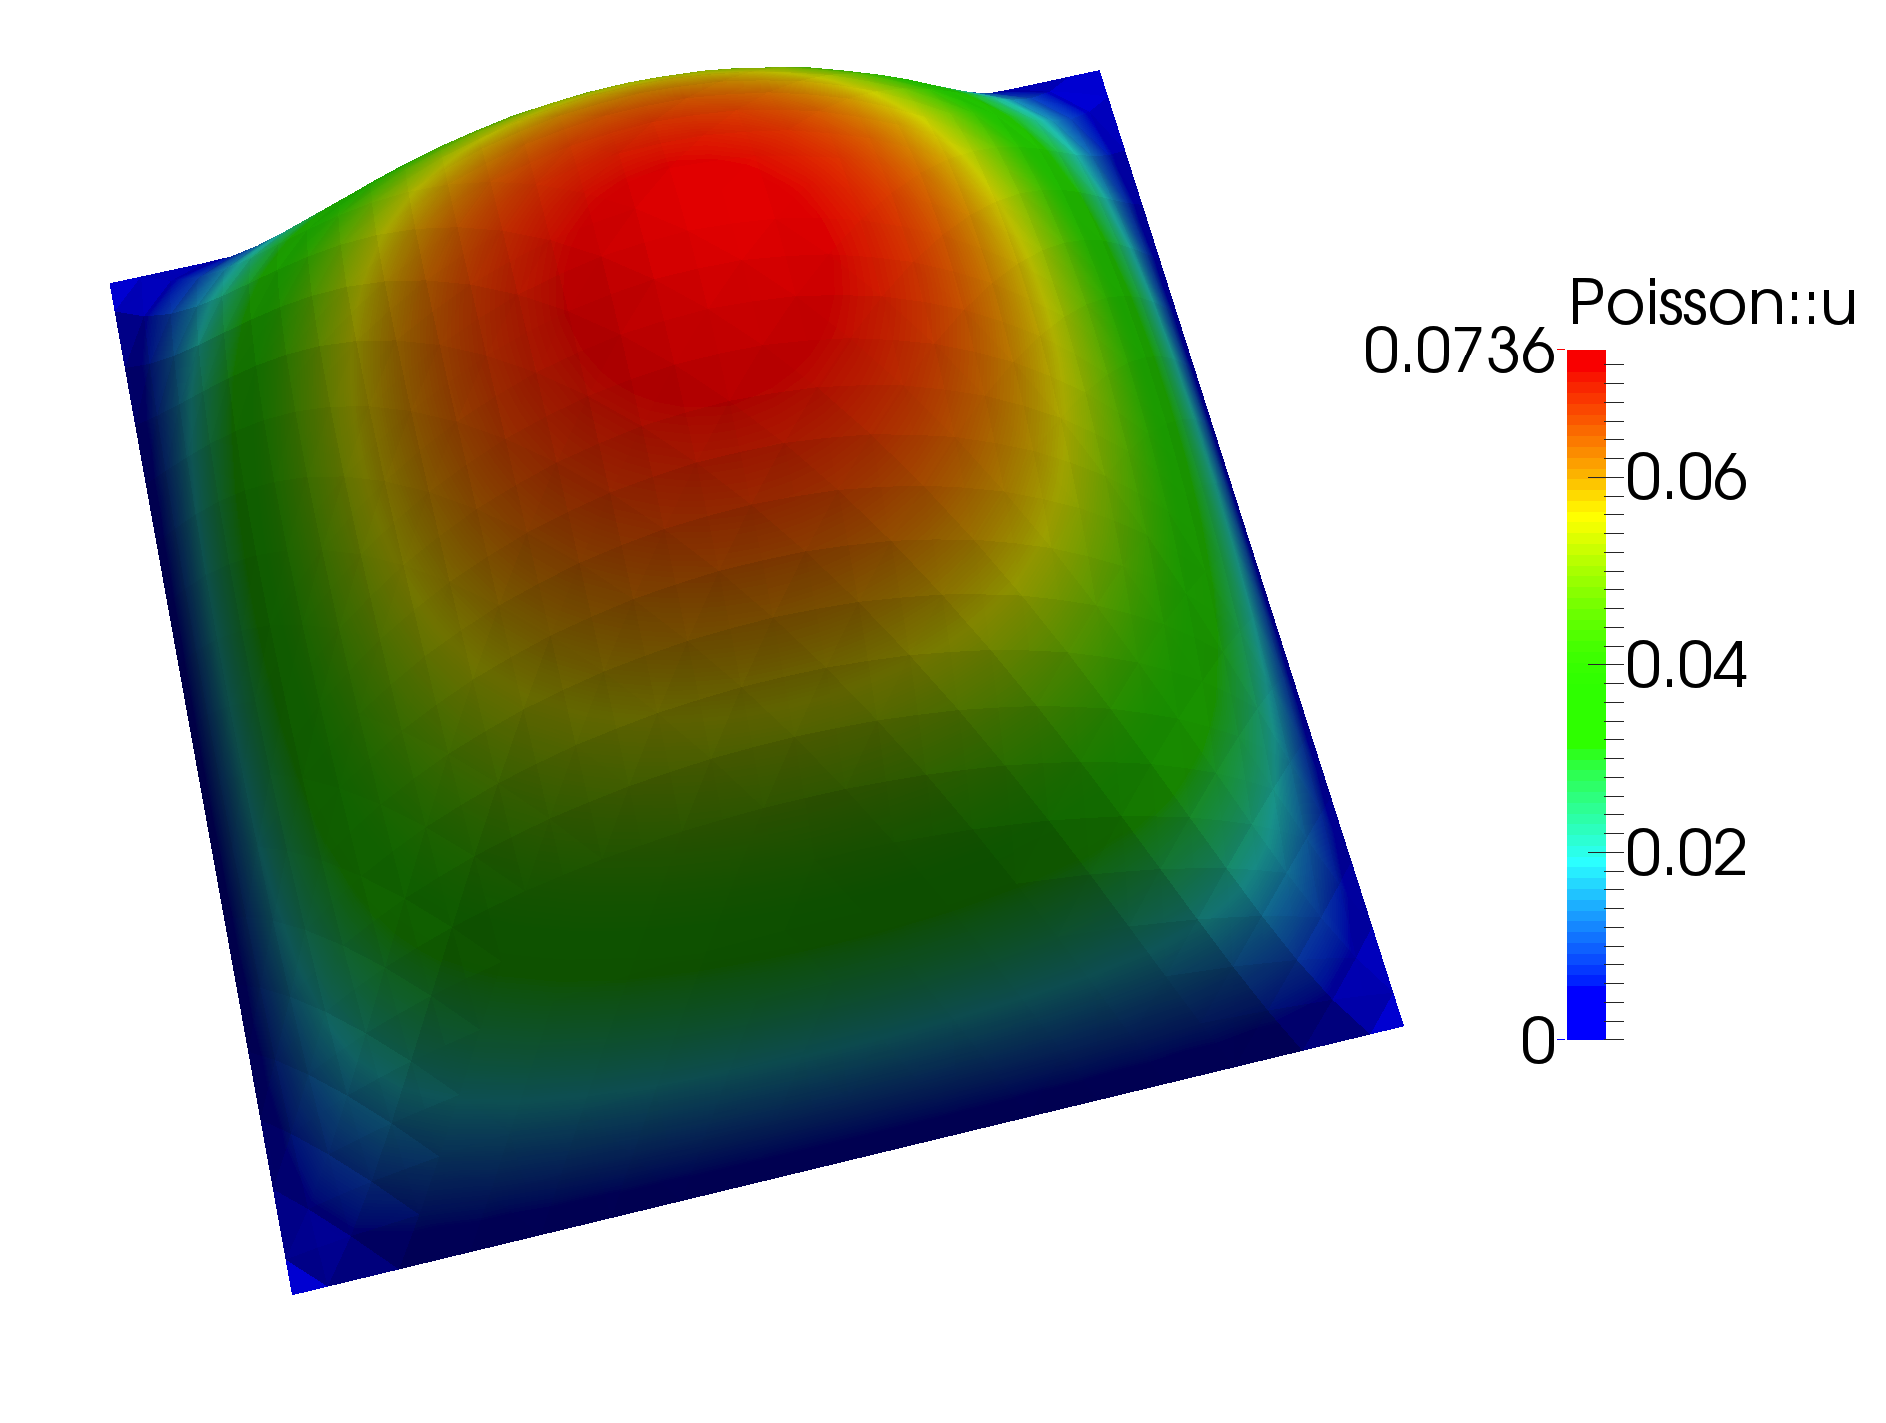
\includegraphics[width=.8\textwidth]{figures/poisson_simple.png}
  \caption{\protect\small The FEM solution of Poisson's equation on the unit square
    with unit forcing and homogeneous dirichlet boundary conditions.
    This version solves the problem using piecewise linear elements (P1)
    on a $32\times 32$ crossed triangular mesh. The mesh can be seen
    in the facets of the solution.}
  \label{fig:simple_poisson}
\end{figure}

\subsection{Step-by-step instructions for building poisson.tfml}
\label{sec:step-step-instr}

To really begin to understand and use \TF{}, however, we need to
construct and populate our own version of \texttt{poisson.tfml} from
which we can then modify and extend later in the themes and variations
section.  Because of the graphical nature of \texttt{diamond} the
following set of steps will probably take longer to read than it
actually takes to set the problem up.  But to be completely pedantic,
here are all the steps spelled out with screendumps to compare.

\begin{steps}{Step}
\item  create an empty directory somewhere and start diamond
\begin{lstlisting}[style=bash]
$ mkdir mypoisson
$ cd mypoisson
$ diamond poisson.tfml & 
\end{lstlisting}%$
This will pop-up a
diamond window with an empty \texttt{tfml} file.
It should look something like
\begin{figure}[h]
  \centering
  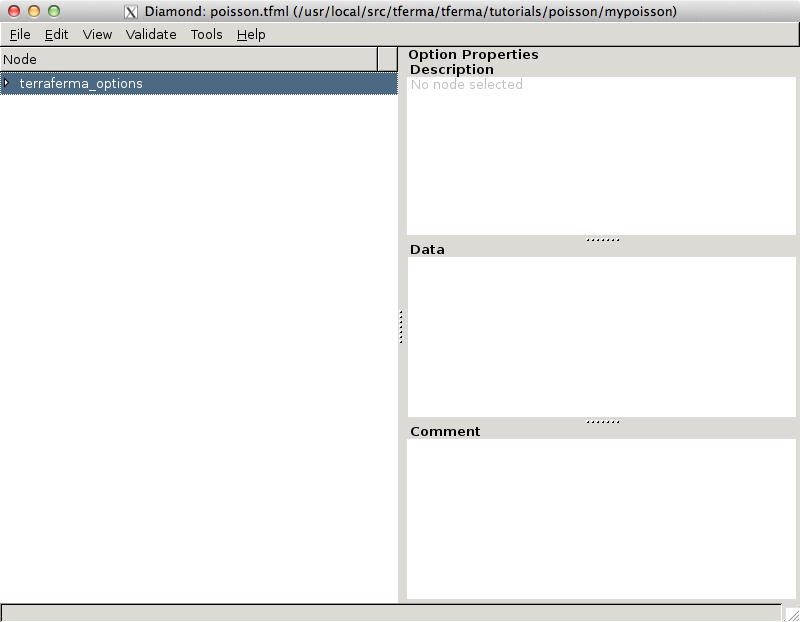
\includegraphics[width=\diamondwidth]{figures/screendumps/diamond_poisson_00.png}
  \caption{0th level diamond window}
  \label{fig:diamond-poisson-0}
\end{figure}
\pagebreak
\item Unfold the terraferma-options tab to view the top level options
  for setting \textbf{geometry}, \textbf{io}, \textbf{system}.  Required fields with
    incomplete options are highlighted in blue.
\begin{center}
  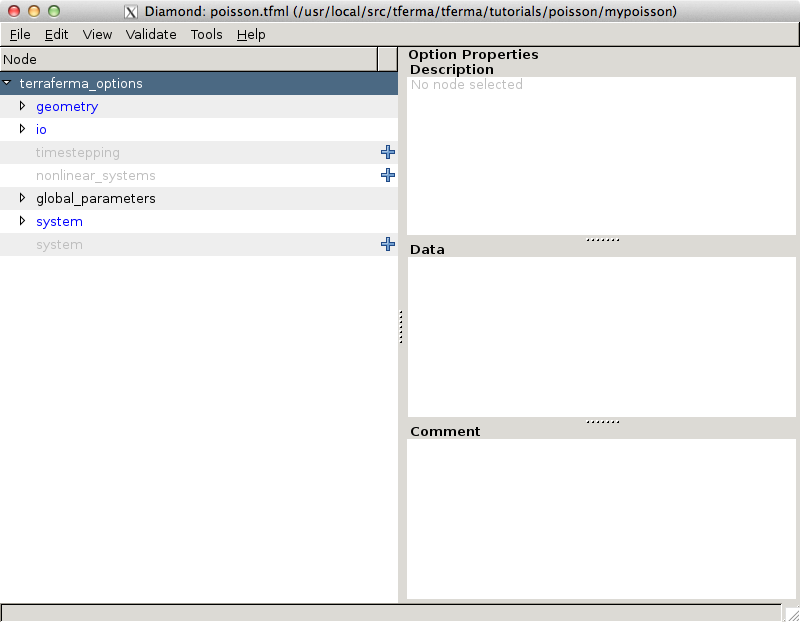
\includegraphics[width=\diamondwidth]{figures/screendumps/diamond_poisson_01.png}
\end{center}

\item\textbf{ Set Geometry option: dimension}: Unfold the
  \textbf{geometry tab} and choose \textbf{dimension}.  This is the
  physical dimension of the domain (1-D, 2-D, 3-D) and can be set only
  once (as it determines the size of other options).  In the right
  hand \textbf{data} window choose 2.
\begin{center}
  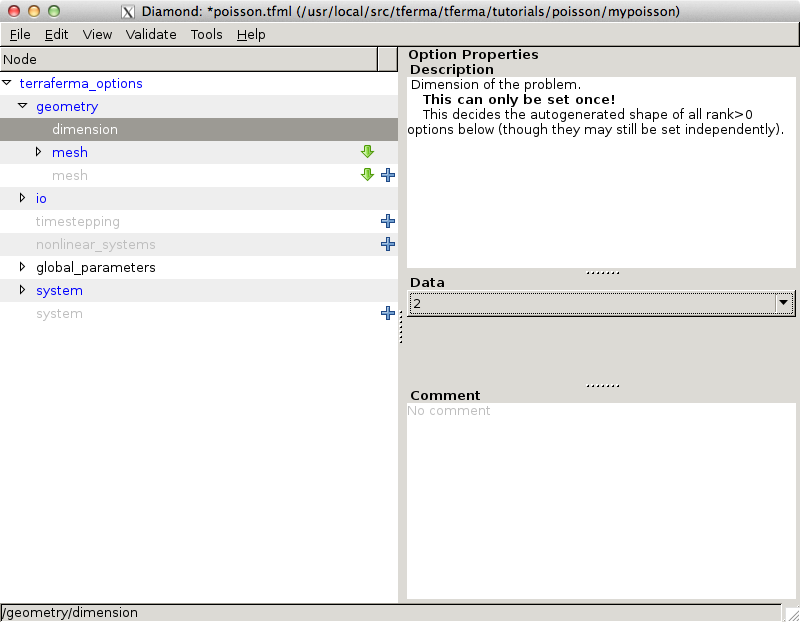
\includegraphics[width=\diamondwidth]{figures/screendumps/diamond_poisson_02a.png}    
  \end{center}

\item \textbf{Set Geometry option: Mesh} Select the Mesh tab and
  use the green arrow to choose the default name Mesh.  
  \begin{center}
    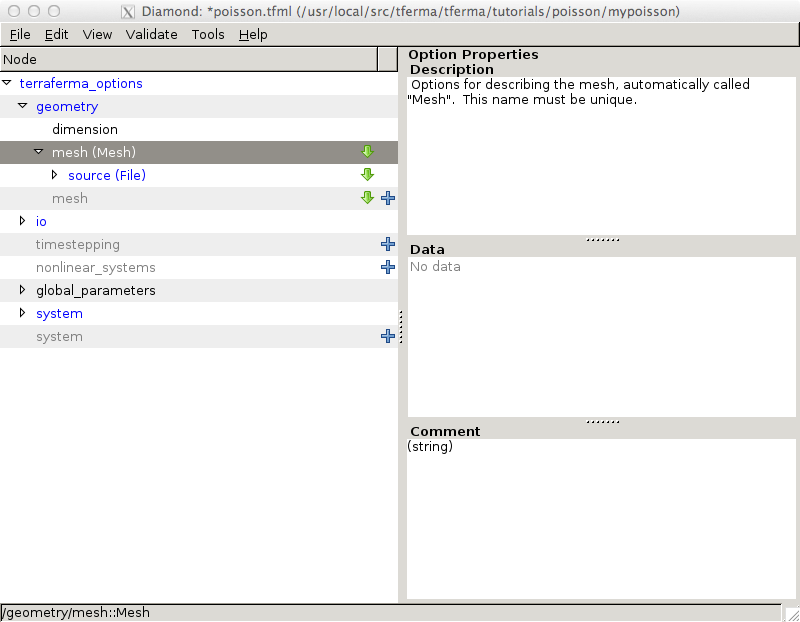
\includegraphics[width=\diamondwidth]{figures/screendumps/diamond_poisson_03a.png}
  \end{center}

Now unfold the \textbf{mesh} tab to expose the \textbf{source} tab and
using the green arrow choose \textbf{source (UnitSquare)} from the
options (default is File).
\begin{center}
  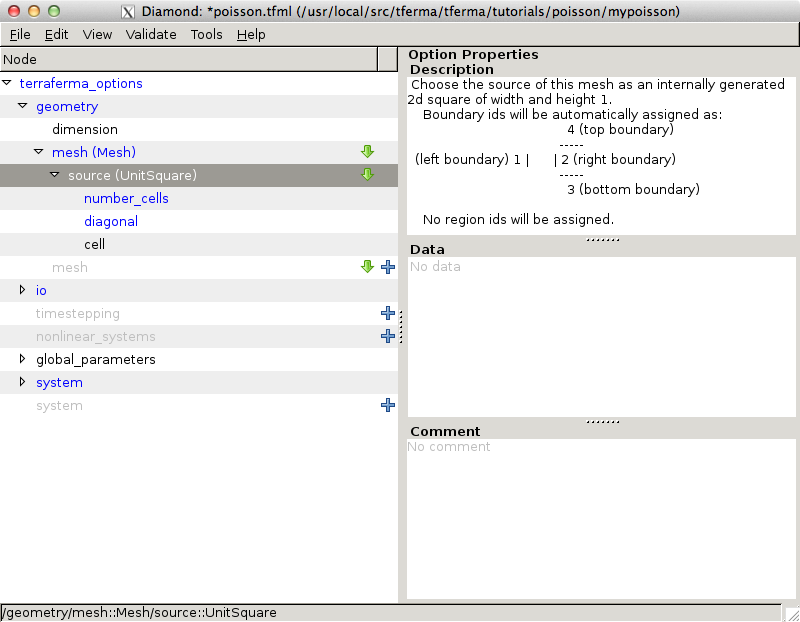
\includegraphics[width=\diamondwidth]{figures/screendumps/diamond_poisson_03b.png}
\end{center}
This will expose two more fields, \textbf{number\_cells} and
\textbf{diagonal}.

Choose \textbf{number\_cells} and set each field to 32 (for a
$32\times32$ cell mesh.
\begin{center}
    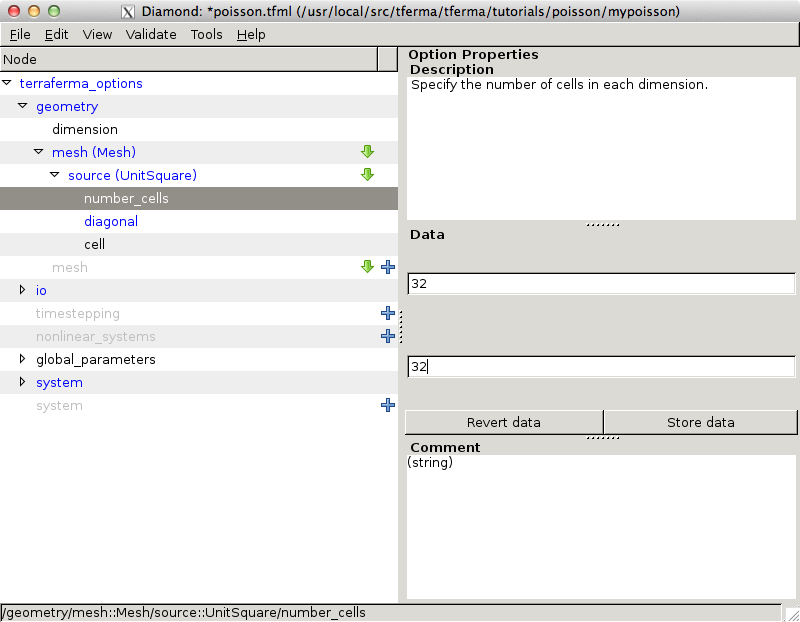
\includegraphics[width=\diamondwidth]{figures/screendumps/diamond_poisson_03c.png}
\end{center}

Then choose \textbf{diagonal} and set to \textbf{right/left}. 
\begin{center}
    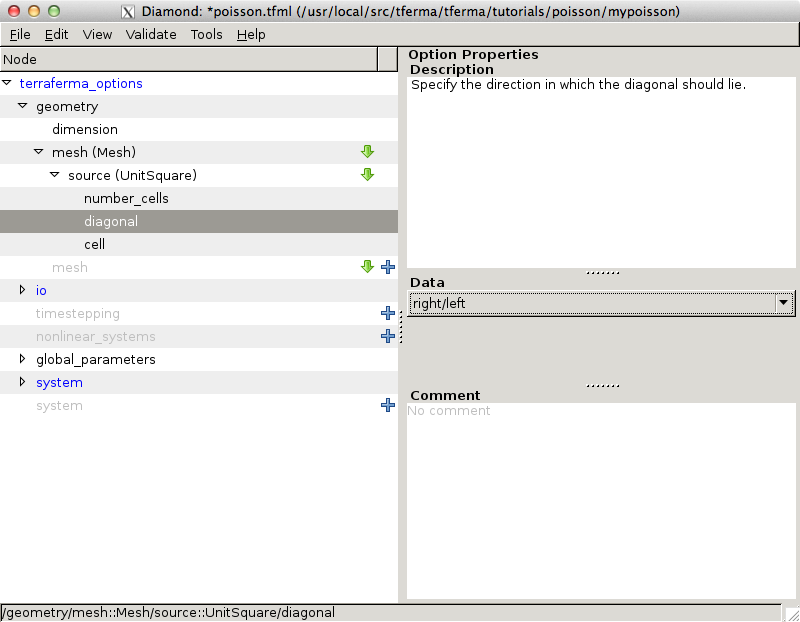
\includegraphics[width=\diamondwidth]{figures/screendumps/diamond_poisson_03d.png}
\end{center}
This completes all the required choices for setting the geometry and
the geometry tab should have changed from blue to black. At this point
(or before) you should save your file (and you can refold the geometry
tab). Also hopefully by this point it
  should be relatively clear how to maneuver around the diamond
  window.  
\item \textbf{Setting io parameters:}  The next step is to set IO
  parameters.
First unfold both the \textbf{io} then \textbf{visualization} tabs.
\textbf{output\_base\_name} is a required field and should be blue. It sets the
rootname of any output file.  Set this to \emph{poisson}.
\textbf{Caution!} do not include a line return after the string poisson. 
\begin{center}
    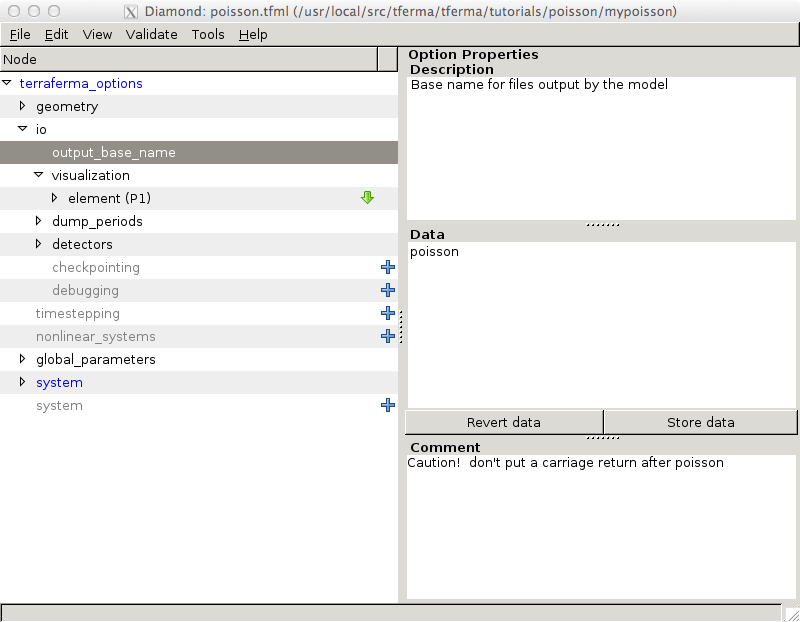
\includegraphics[width=\diamondwidth]{figures/screendumps/diamond_poisson_04.png}
\end{center}
\textbf{visualization} sets the default element used in the vtk files
for visualizing fields.  This is optional and defaults to P1 (piecewise
linear functions) which will be adequate for this problem which will
also use P1 elements.

This completes the \textbf{io} options tree.
%{\samepage
\item \textbf{Setting the System:}  The \textbf{system} is the heart of
  \TF{} and includes all the choices of fields, elements,
  coefficients, boundary
  conditions and solvers.  You can have multiple systems in any
  problem but each one needs a \textbf{name}, a \textbf{mesh} and a
  \emph{unique}, global \textbf{ufl\_symbol}.  Start by setting the system
  name to \texttt{poisson}.
\textbf{Note!}  For any name field you will need to hit return in
diamond to set it,  other fields you should not include carriage returns. 
\begin{center}
    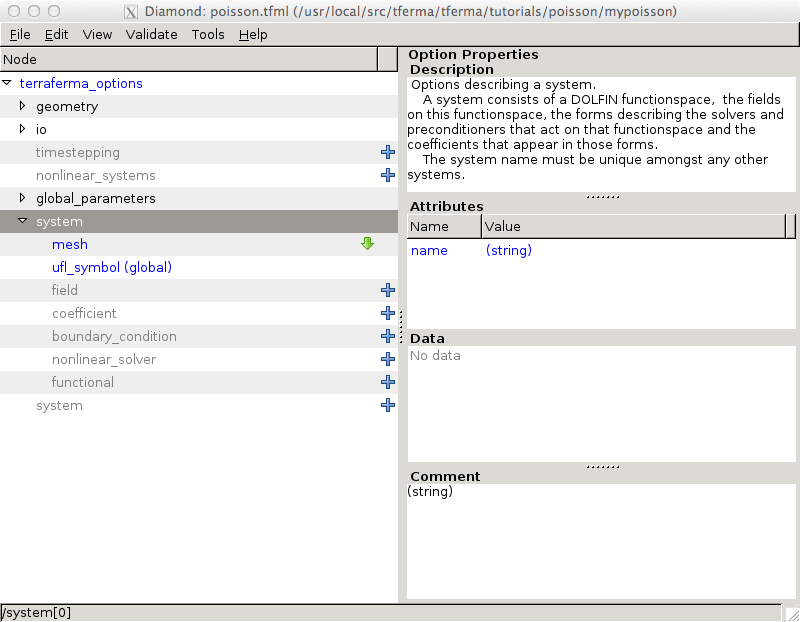
\includegraphics[width=\diamondwidth]{figures/screendumps/diamond_poisson_05a.png}
\end{center}
then choose  the \textbf{mesh} name to be consistent with what you set in
geometry (Mesh), and choose \textbf{ufl\_symbol (global)} and set it to
\texttt{us}. (Later on we will distinguish between system symbols
which include all fields in a system, and the individual field
symbols).
\begin{center}
    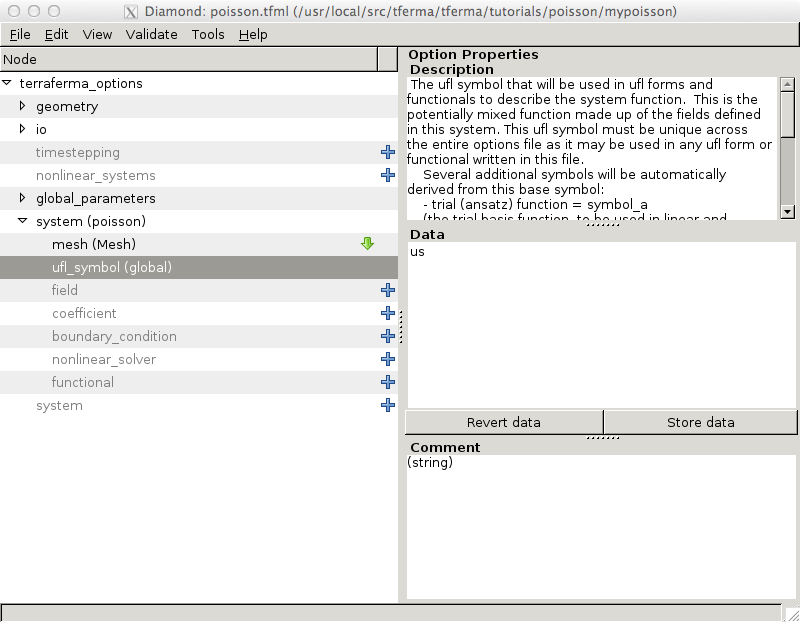
\includegraphics[width=\diamondwidth]{figures/screendumps/diamond_poisson_05c.png}
\end{center}
%}
\item \textbf{Setting the field:} Next step is to actually describe
  the field (function) or fields we are trying to solve in each
  system.  Poisson has only one field and which we will enable by
  clicking the $+$ next to the greyed out \textbf{field} tab and
  unfold the new field tab.
\begin{center}
    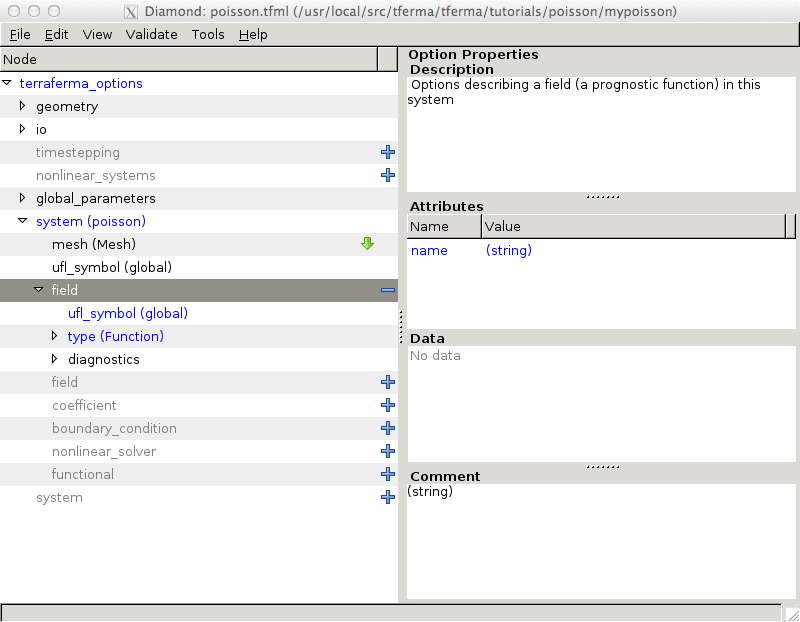
\includegraphics[width=\diamondwidth]{figures/screendumps/diamond_poisson_06a.png}
\end{center}
Each field requires both a \textbf{name} and a unique, global
\textbf{ufl\_symbol}.  Here set the field name to \texttt{ufield} and
the ufl\_symbol to \texttt{u}.
\begin{center}
    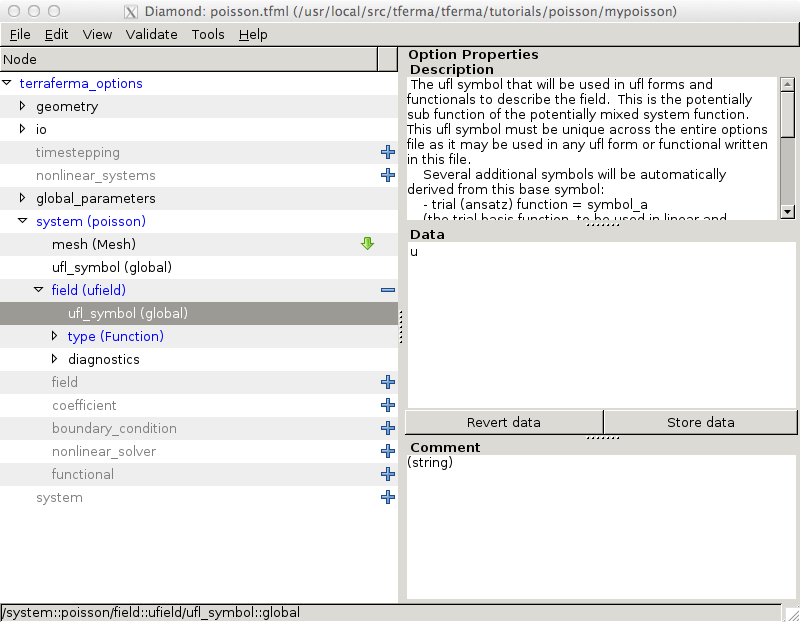
\includegraphics[width=\diamondwidth]{figures/screendumps/diamond_poisson_06c.png}
\end{center}
\item \textbf{Setting Field attributes:} Once named we next need to
  set critical attributes on the field including its \textbf{rank}
  (scalar, vector or tensor valued field), the \textbf{element},
  \textbf{initial conditions} and \textbf{boundary conditions.} Unfold
  the \textbf{Function} tab and its sub tab \textbf{rank}
\begin{center}
    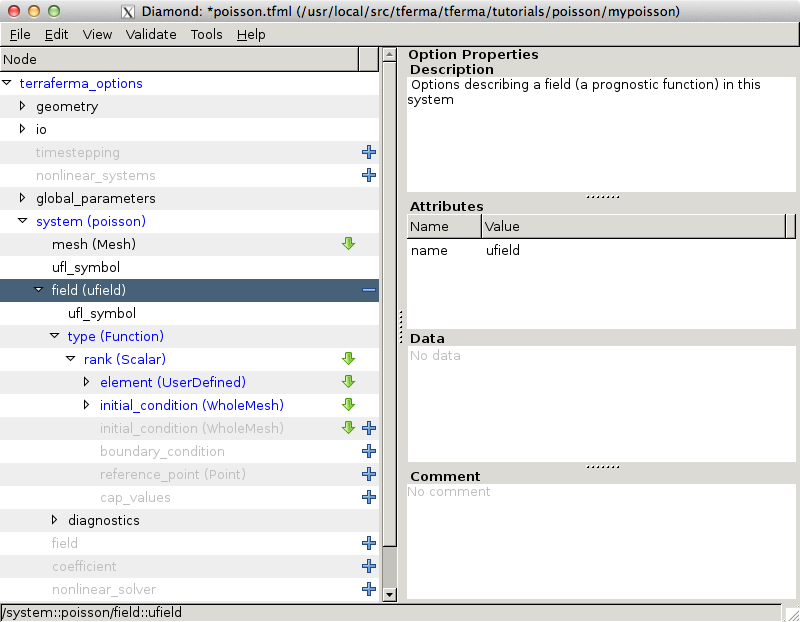
\includegraphics[width=\diamondwidth]{figures/screendumps/diamond_poisson_07a.png}
\end{center}
\textbf{rank} is already set to Scalar (green arrows could choose
vector or tensor). Use the green arrows to choose the built in
\textbf{element} P1 (which automatically chooses an element family
``CG'' (continuous galerkin, or Lagrange element) of degree 1.
\begin{center}
    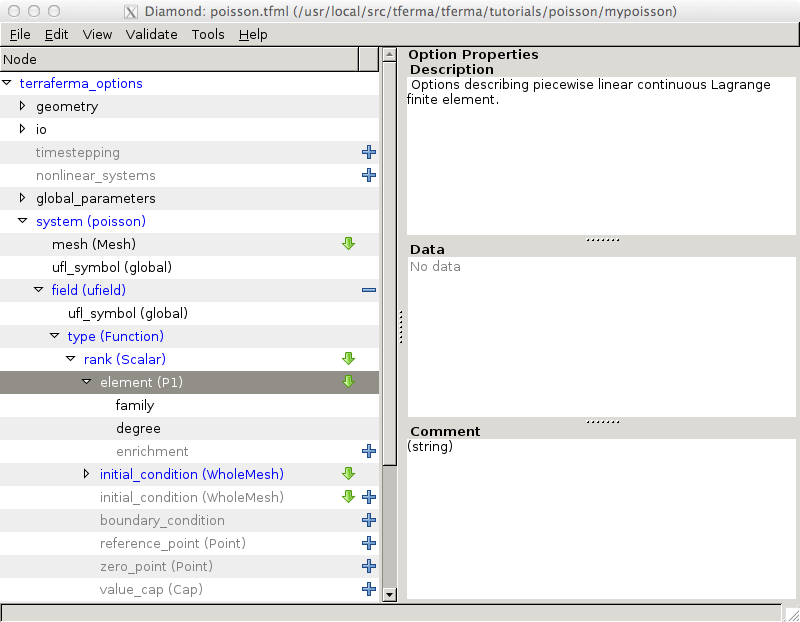
\includegraphics[width=\diamondwidth]{figures/screendumps/diamond_poisson_07b.png}
\end{center}
\item \textbf{Setting initial conditions:} Because we
  often use iterative solvers even on steady state problems, we need
  to initialize all fields with an initial condition.  Here we will
  just set it to a constant 0 over the whole mesh.  Unfold the
  \textbf{initial\_condition (WholeMesh)} tab and set the constant to
  \texttt{0.}
\begin{center}
    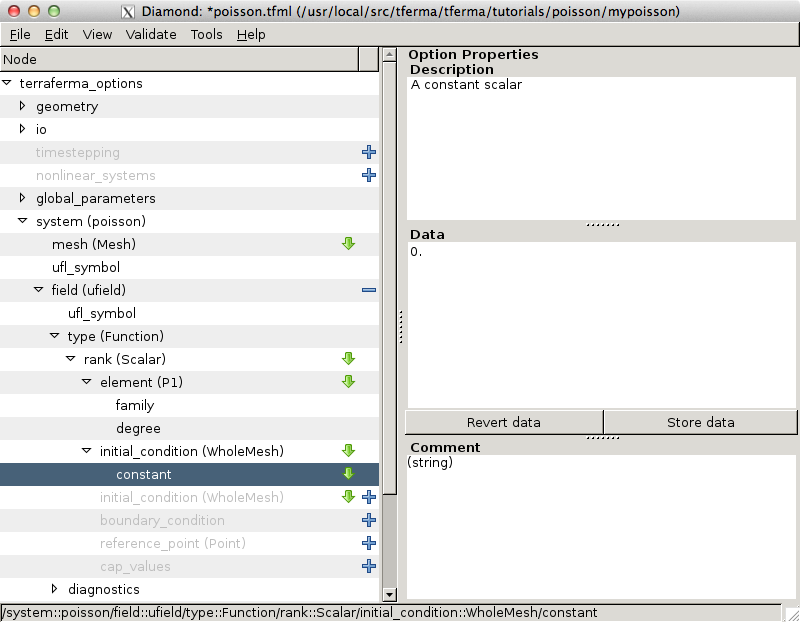
\includegraphics[width=\diamondwidth]{figures/screendumps/diamond_poisson_07c.png}
\end{center}
\item \textbf{Setting Boundary conditions:} Now we need to set
  Dirichlet conditions on the field so that it is zero on all four
  boundaries. First, activate the \textbf{boundary\_condition} tab,
  give it a name (\texttt{ZeroBCs}) and
  unfold all the suboptions. 
\begin{center}
    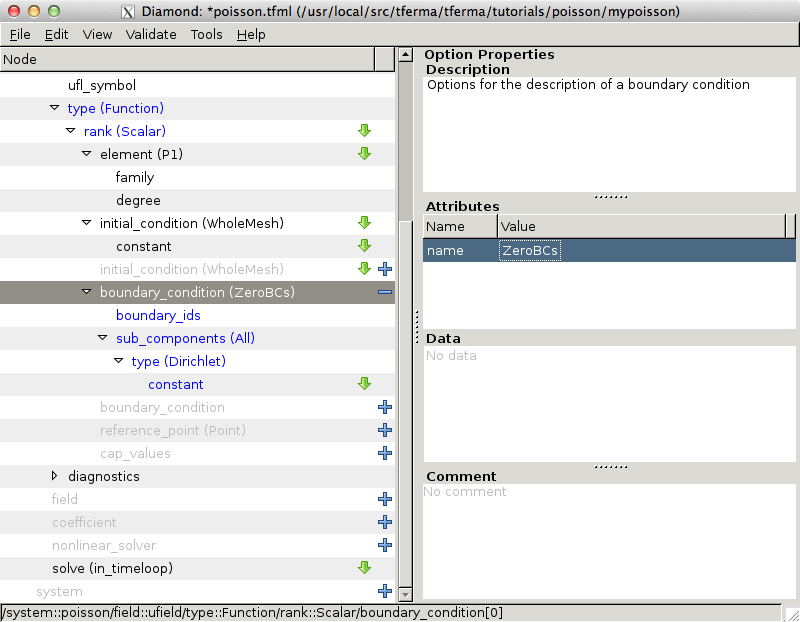
\includegraphics[width=\diamondwidth]{figures/screendumps/diamond_poisson_08b.png}
\end{center}
This will expose the options \textbf{boundary\_ids} which identify
which boundaries are affected, and \textbf{Type (Dirichlet)} which
let's you set a function that evaluates the dirichlet BCs.  For the
unit square,  the Boundary ID's are shown with the \textbf{source
  (UnitSquare)} tab (see Step 4, second figure).  Here we'll set all
of them by putting \texttt{1 2 3 4} in \textbf{boundary\_ids}.  
\begin{center}
    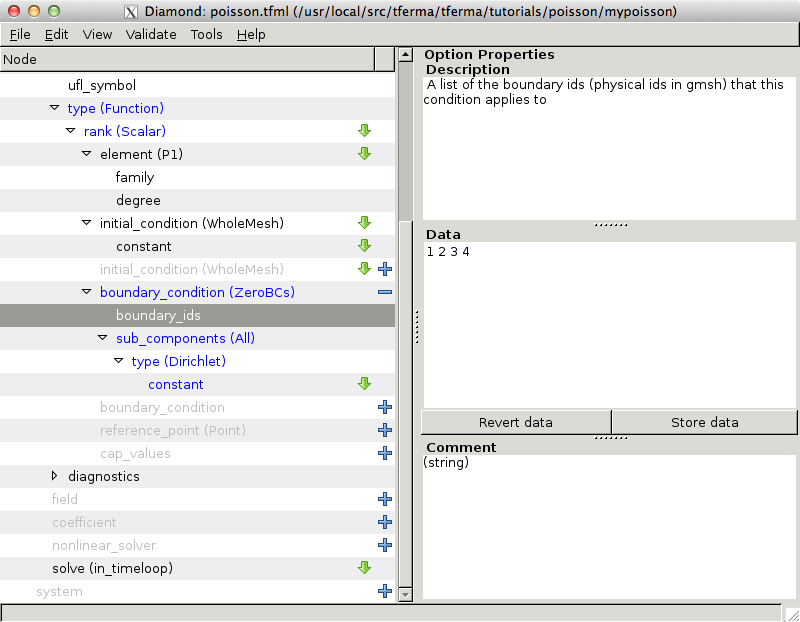
\includegraphics[width=\diamondwidth]{figures/screendumps/diamond_poisson_08c.png}
\end{center}
and we will set the \texttt{type (Dirichlet)} to a constant function
with value 0.
\begin{center}
    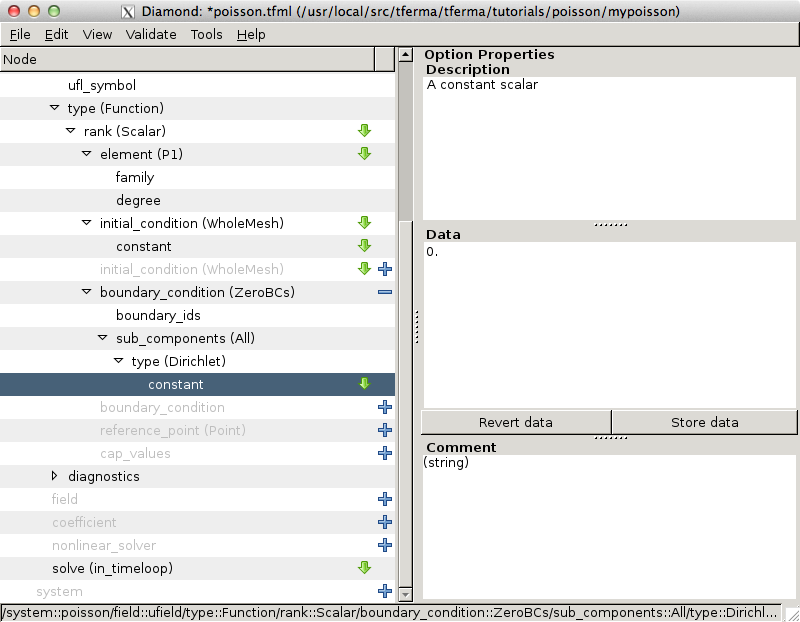
\includegraphics[width=\diamondwidth]{figures/screendumps/diamond_poisson_08d.png}
\end{center}
This completes the \textbf{Function} tab, which you can refold.
\item \textbf{Setting Diagnostics on a field:}  If you want to actually visualize
  or get output about a field, you'll need to add it to the
  diagnostics.  Unfold the \textbf{diagnostics} tab and activate
  \textbf{include\_in\_visualization} and
  \textbf{include\_in\_statistics}. Other options are available.
\begin{center}
    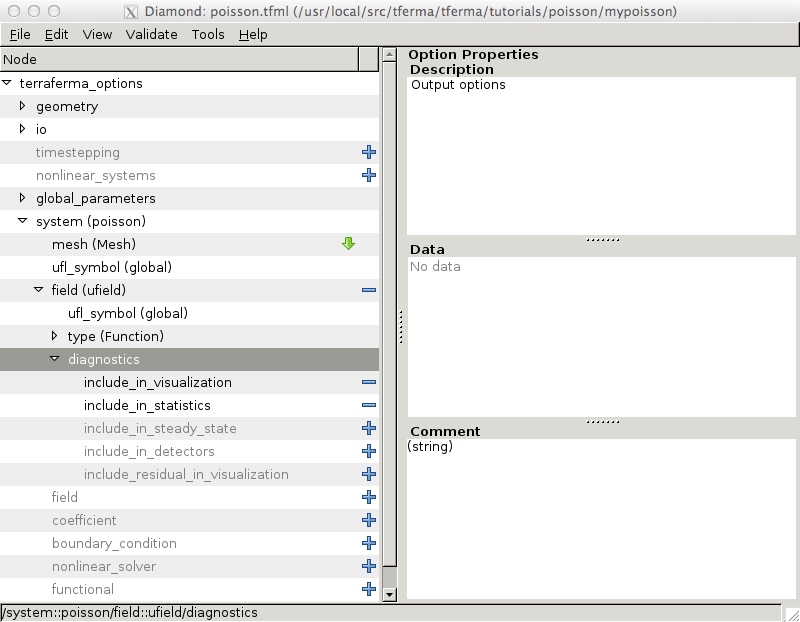
\includegraphics[width=\diamondwidth]{figures/screendumps/diamond_poisson_09.png}
\end{center}
This completes the \textbf{field} tab
\item \textbf{Setting the RHS coefficient $f$:} To solve Poisson, we
  need to give the system a rhs function $f(\vec{x})$ which in this
  case is a constant $f=1$.  In ufl notation,  $f$ is a
  \emph{coefficient} in the form that can be evaluated at any point in
  the domain.  To set $f$, activate the \textbf{coefficient} tab and
  give it a name (here \texttt{rhs}) and unfold. We will also need to
  give it a  ufl symbol (\texttt{f}). 
\begin{center}
    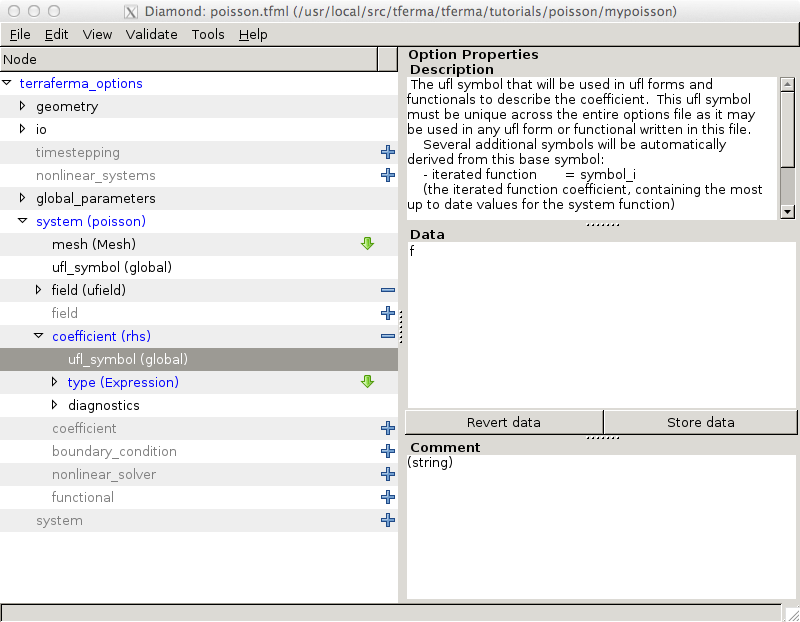
\includegraphics[width=\diamondwidth]{figures/screendumps/diamond_poisson_10b.png}
\end{center}
 To evaluate \texttt{f}, we need to set the \textbf{type} to
\textbf{Constant} using the drop down arrows, then continue to unfold
until you can set the constant value to 1.
\begin{center}
    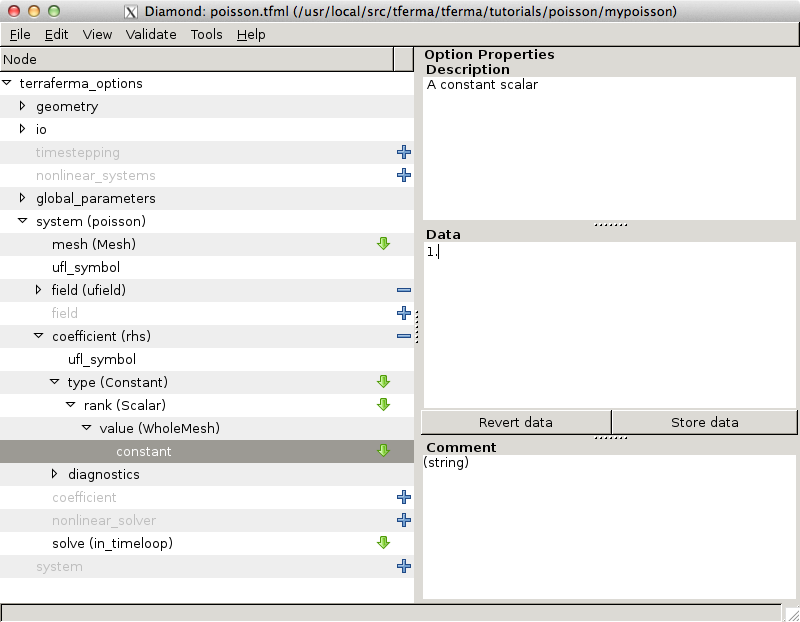
\includegraphics[width=\diamondwidth]{figures/screendumps/diamond_poisson_10c.png}
\end{center}
This completes the coefficient field.
\item \textbf{Setting the solver (and equations):}  The last set of
  choices involve setting the solvers for the system.  In \TF{}, the
  actual equations we want to solve are part of the solver as each
  solver acts as an operator over the fields (and you can have
  multiple solvers in a system).  Here we will implement Poisson using
  PETSc's Newton solver SNES.  

Start by activating the \textbf{nonlinear\_solver} tab, name the
solver (\texttt{Solver}) and unfold.
\begin{center}
    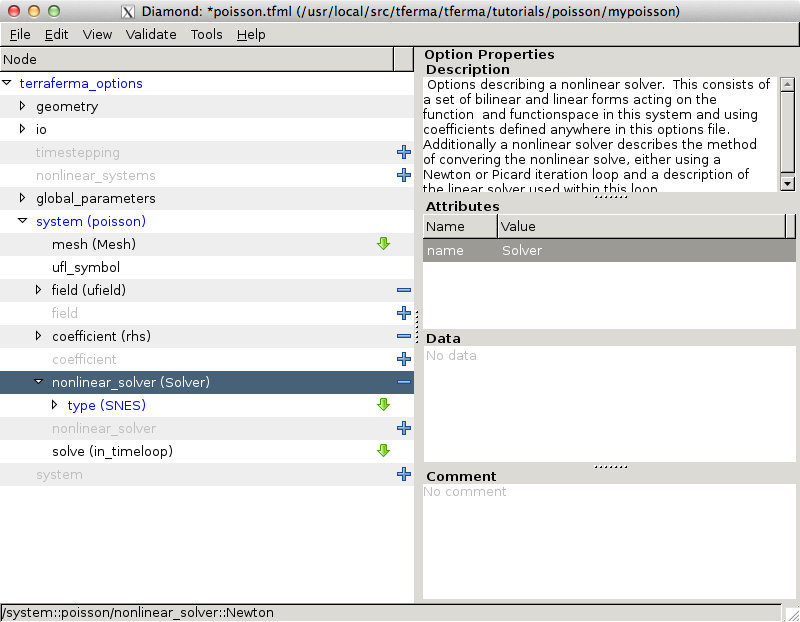
\includegraphics[width=\diamondwidth]{figures/screendumps/diamond_poisson_11a.png}
\end{center}
We will use the default type \textbf{SNES} which is PETSc's Scaleable
Non-linear Equation Solver which provides a large range of Newton and
quasi-newton schemes with control.
\item \textbf{Setting the SNES options:} Unfold the \textbf{type
    (SNES)} tab to show all the required options for a non-linear
 Newton  solver
\begin{center}
    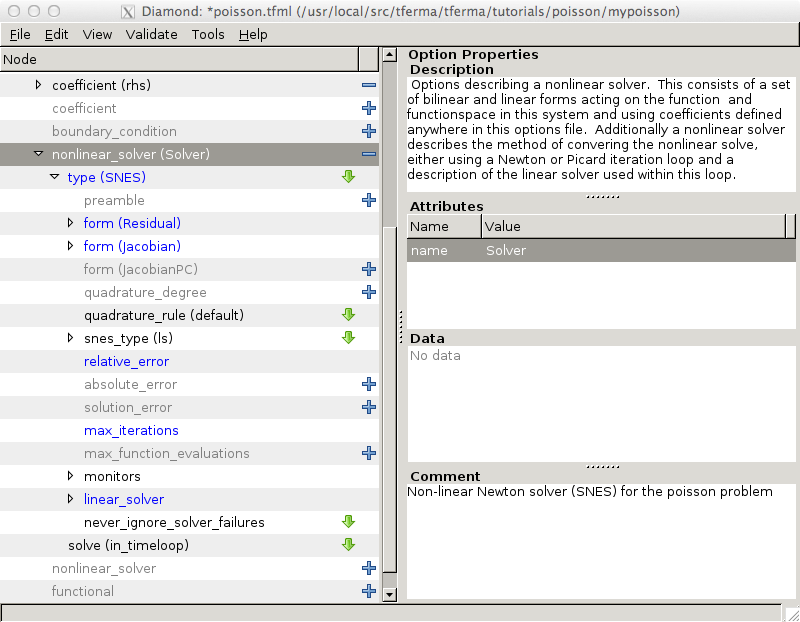
\includegraphics[width=\diamondwidth]{figures/screendumps/diamond_poisson_11b.png}
\end{center}
which include weak forms for the \textbf{Residual}, and
\textbf{Jacobian}, parameters to control convergence such as
\textbf{relative\_tolerance} and \textbf{maximum\_iterations} as well
as choice of \textbf{linear\_solvers} for the inner solver.

First we will set the weak form for the \textbf{form (Residual)}.
First highlight the  \textbf{form (Residual)} tab and in the
\textbf{Data} window add the following piece of ufl
\begin{lstlisting}[style=ufl]
F   = (inner(grad(u_t), grad(u_i)) - u_t*f)*dx
\end{lstlisting}
to define the weak form of the residual given on field \texttt{u} and
coefficient \texttt{f}.  The subscripted ufl symbols are automatically
generated by \TF{}. 
\begin{center}
    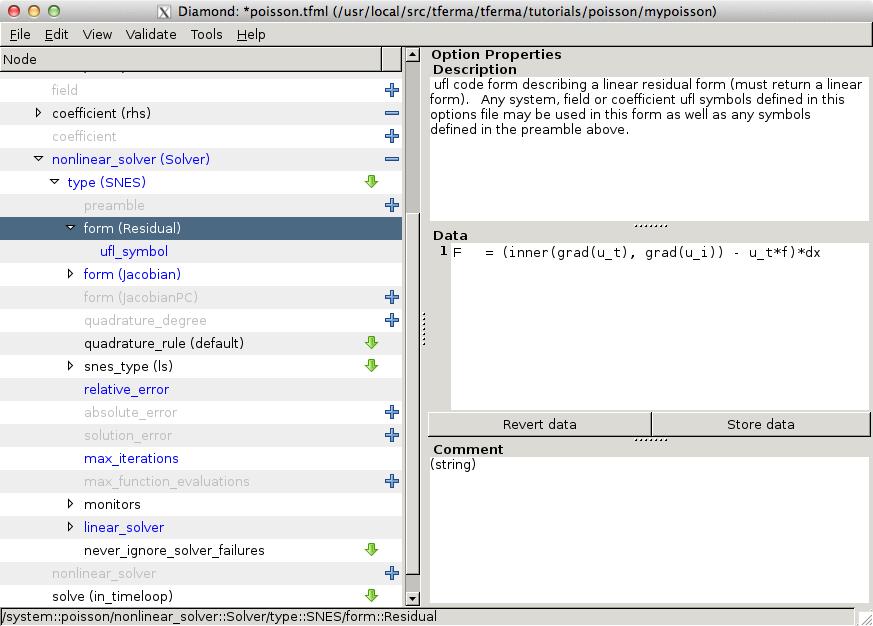
\includegraphics[width=\diamondwidth]{figures/screendumps/diamond_poisson_11c.png}
\end{center}
Also unfold the \textbf{form (Residual)} tab and set the
\textbf{ufl\_symbol} for the form to \texttt{F}

To set the Jacobian choose  the \textbf{form (Jacobian)} tab and add
the ufl
\begin{lstlisting}[style=ufl]
J = derivative(F,us_i,us_a)
\end{lstlisting}
and set its ufl symbol to \texttt{J}.  Note the derivative is taken
with respect to the \textbf{System} ufl symbol \texttt{us} not the
field (this will become more obvious with other problems).
\begin{center}
    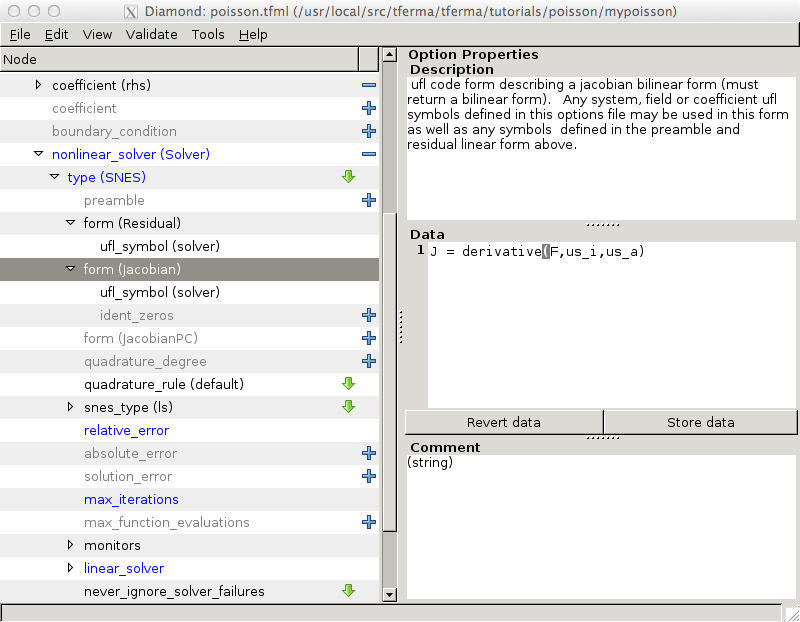
\includegraphics[width=\diamondwidth]{figures/screendumps/diamond_poisson_11d.png}
\end{center}

Now set \textbf{relative\_error} to \texttt{1.e-6} and
\textbf{max\_iterations} to \texttt{20} (and we won't need more than 1
actually for this problem) and unfold the \textbf{linear\_solver} tab
\begin{center}
    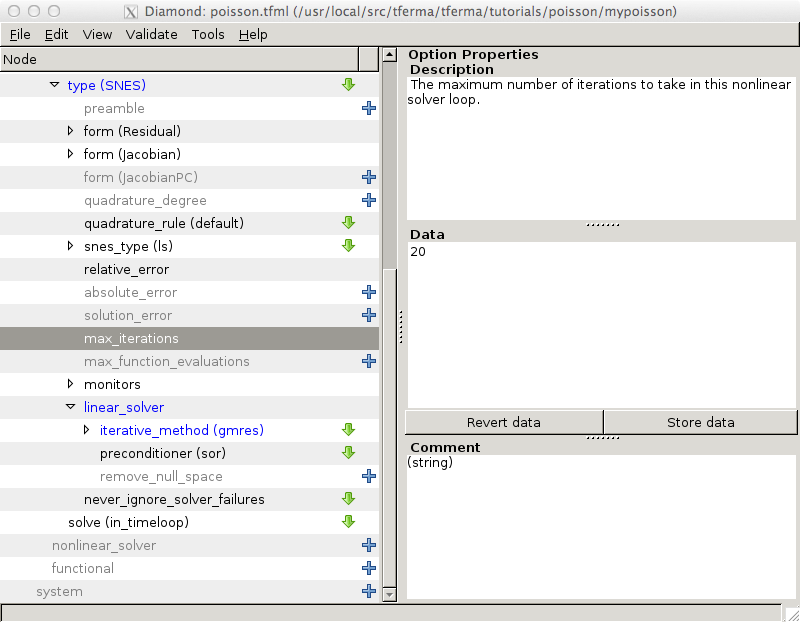
\includegraphics[width=\diamondwidth]{figures/screendumps/diamond_poisson_11e.png}
\end{center}
\item \textbf{Setting the Linear solver options:} Finally we need to
  set options for the inner linear solver.  For a small 2-D problem
  it's nearly impossible to beat sparse direct methods so we'll start
  with those.  Every linear solver has 2 components an
  \textbf{iterative\_method} (which is a PETSc KSP) and a
  \textbf{preconditioner} (a PETSc PC).  The appropriate (KSP,PC)
  pair for a direct solver is (preonly, lu), i.e a sparse-lu decomposition as
  a pre-conditioner (which is a direct solve) and no iterative
  method.  In \TF{} we use the green drop-down arrows to choose
  \textbf{linear\_solver} to be \texttt{preonly}, and
  \textbf{preconditioner} to be \texttt{lu}, which will default to the
  sparse direct solver \texttt{umfpack} (which is what is used in
  matlab).  Other direct solver packages such as mumps can also be chosen.
\begin{center}
    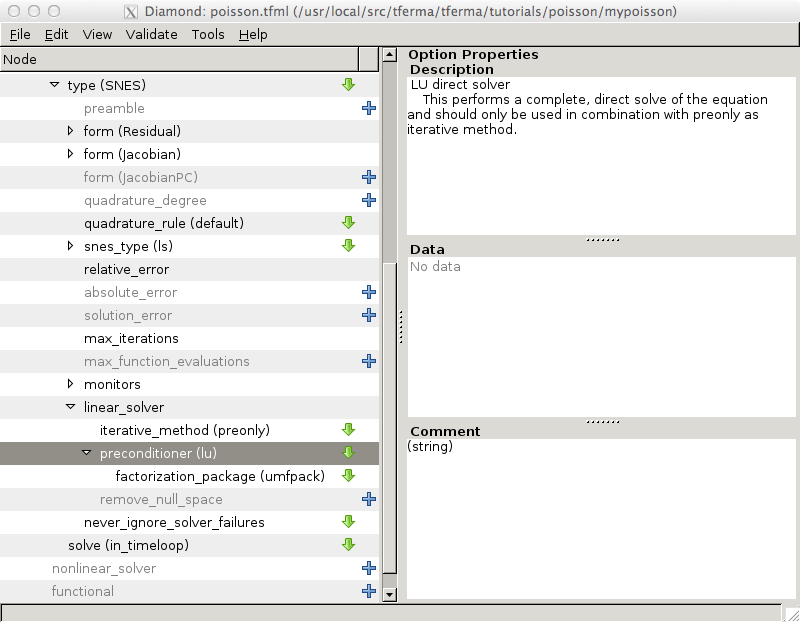
\includegraphics[width=\diamondwidth]{figures/screendumps/diamond_poisson_12a.png}
\end{center}
This completes all the choices required to build
\texttt{poisson.tfml}. \textbf{Save your file}, cross your fingers and see if
we can build this.
\item \textbf{Building and running your model:}  The instructions are
  given at the beginning of Section \ref{sec:ch2-solution-using-tf} but to
  repeat
\begin{lstlisting}[style=Bash]
$ tfbuild poisson.tfml
$ cd build
$ make run 
\end{lstlisting} %$
Compilation the first time requires automatic generation of C++ code from
the ufl forms (using FFC), then creating wrappers to link into the
base \TF libraries.  Once the code has been compiled however, changes
to run-time parameters will not force a recompile or relinking and
\lstinline[style=Bash]´$ make run´ %$
will be much quicker.  Any change to \texttt{ufl} or expressions that
require recompilation will force a rebuild automatically.
\item \textbf{Trouble shooting:} Murphy is the lord of modeling and
  anything that can go wrong will go wrong.  One of the nicer features
  of \TF{} is that it compartmentalizes many of the choices, which can
  help to more rapidly locate errors.  One of the poorer features of
  \TF{} is that the error messages are somewhat cryptic.

As a first cut,  use a good diff tool such as \texttt{meld} (Linux) or
\texttt{opendiff} (MacOSX) to compare your file \texttt{poisson.tfml} to
the working example in
\texttt{\$TF\_HOME/share/terraferma/tutorials/poisson/simple/poisson.tfml}.  You'll be
comparing raw \texttt{.tfml} (which is basically xml) but the diffs
should be small.  Simple things to watch out for are
\begin{itemize}
\item Make sure all the required fields are filled in (no blue fields)
\item Extra carriage returns in ufl symbols.
\item Syntax errors in ufl forms.  These errors will be generated
  during the code generation step by FFC.  Read the FFC output
  carefully to try and identify the problem.  The problem will most
  likely lie in the ufl for the weak forms of the residual (or Jacobian).
\item Syntax errors in python functions.  Some expressions can be
  written as small python functions.  If the python path is not set
  correctly or python errors are introduced, these will throw run-time errors.
\end{itemize}




 \end{steps}
  
%\lstinline[style=Bash]´$ tfbuild <filename>.tfml´.




\section{Themes and Variations}
\label{sec:themes-variations}

Given an initial working \texttt{tfml} file, one of the very nice
features of \TF{} is that it becomes usually quite straightforward to
rapidly change your choices to make new models or add new features.
\texttt{tfml} files are just ascii and can be copied to make new
files. In addition,  diamond allows entire options and option
sub-trees to be copied and pasted preserving (with some significant
care) work done in another model.  Here we will start by making some
small modifications to our basic working poisson model, then add some
advanced features such as including non-constant rhs's, boundary
conditions etc.

\subsection{Simple changes}
\label{sec:simple-changes}

Many changes simply change run-time options and have little to no
affect on other model options.  Some obvious ones include
\subsubsection{Changing Resolution}
\label{sec:changing-elements}

To increase the spatial resolution of the mesh, simply edit
\textbf{number\_cells} in the UnitSquare mesh and rerun.

\subsubsection{Changing the mesh}
\label{sec:changing-mesh}

Changing the mesh type itself may or may not be simple.  For example, changing to a rectangle
from a square only requires changing \textbf{source (UnitSquare)} to
\textbf{source (Rectangle)} and editing the appropriate
suboptions. Because the boundary IDs of a square and rectangle are
the same, however, this does not propagate to any other part of the
model. 
\begin{figure}[h!]
  \centering
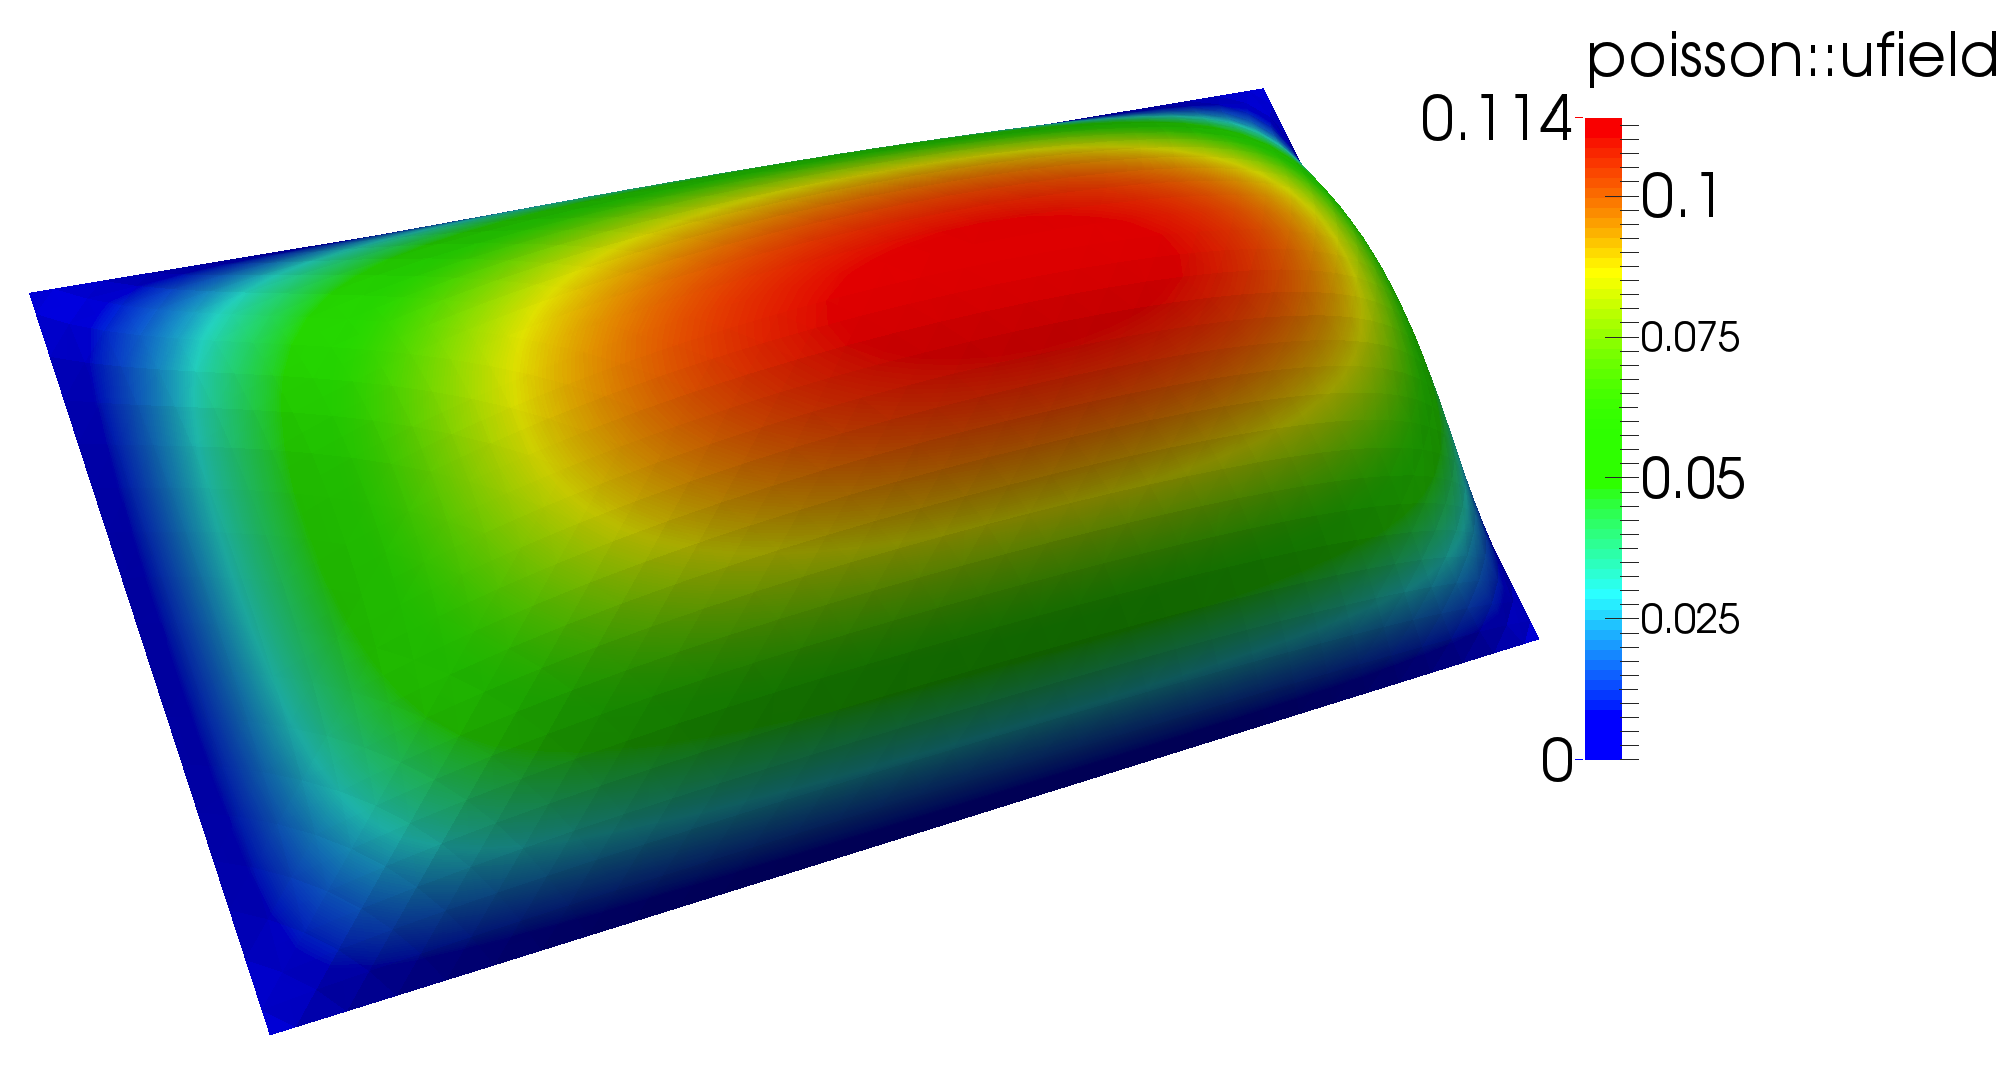
\includegraphics[width=.7\textwidth]{figures/poisson_simple_rectangle}
  \caption{\small Same problem but on a rectangular domain
    $\Omega=[0,2]\times[0,1]$ with $64\times32$ cells.}
\label{fig:poisson_rectangle}
\end{figure}

More generally, we would like to use externally generated meshes.  The
example \texttt{\$TF\_HOME/share/terraferma/tutorials/poisson/gmsh/poisson.tfml}
incorporates a mesh generated using \texttt{gmsh}.  The geometry file
for this mesh is in
\texttt{\$TF\_HOME/share/terraferma/tutorials/poisson/gmsh/mesh/widget.geo}. To convert
for use in TF (Dolfin) use
\begin{lstlisting}[style=Bash]
$ cd $TF_HOME/share/terraferma/tutorials/poisson/gmsh/mesh
$ gmsh -2 -algo del2d widget.geo
$ dolfin-convert widget.msh widget.xml
\end{lstlisting}
the \texttt{gmsh} command generates a 2-D unstructured mesh in
\texttt{widget.msh} and  \texttt{dolfin-convert} generates a dolfin
meshfile in \texttt{.xml} format  that include the mesh geometry as
well as labels for boundary ids.  The actual boundary id's for the
exterior walls (1-6) and interior hole (7) can be found in the geometry file
\texttt{widget.geo}.

To incorporate this mesh into \texttt{poisson.tfml} we simply change
the mesh source to \texttt{Source (File)} and add the file name
relative to the \texttt{tfml} file (i.e. \texttt{../mesh/widget}
without the \texttt{.xml} extension). We also have to edit the
boundary id's in the boundary condition (and add one more boundary
condition for the hole).  A fully worked out example is included and
produces the result shown in Figure \ref{fig:poisson_gmsh}.
\begin{figure}[h!]
  \centering
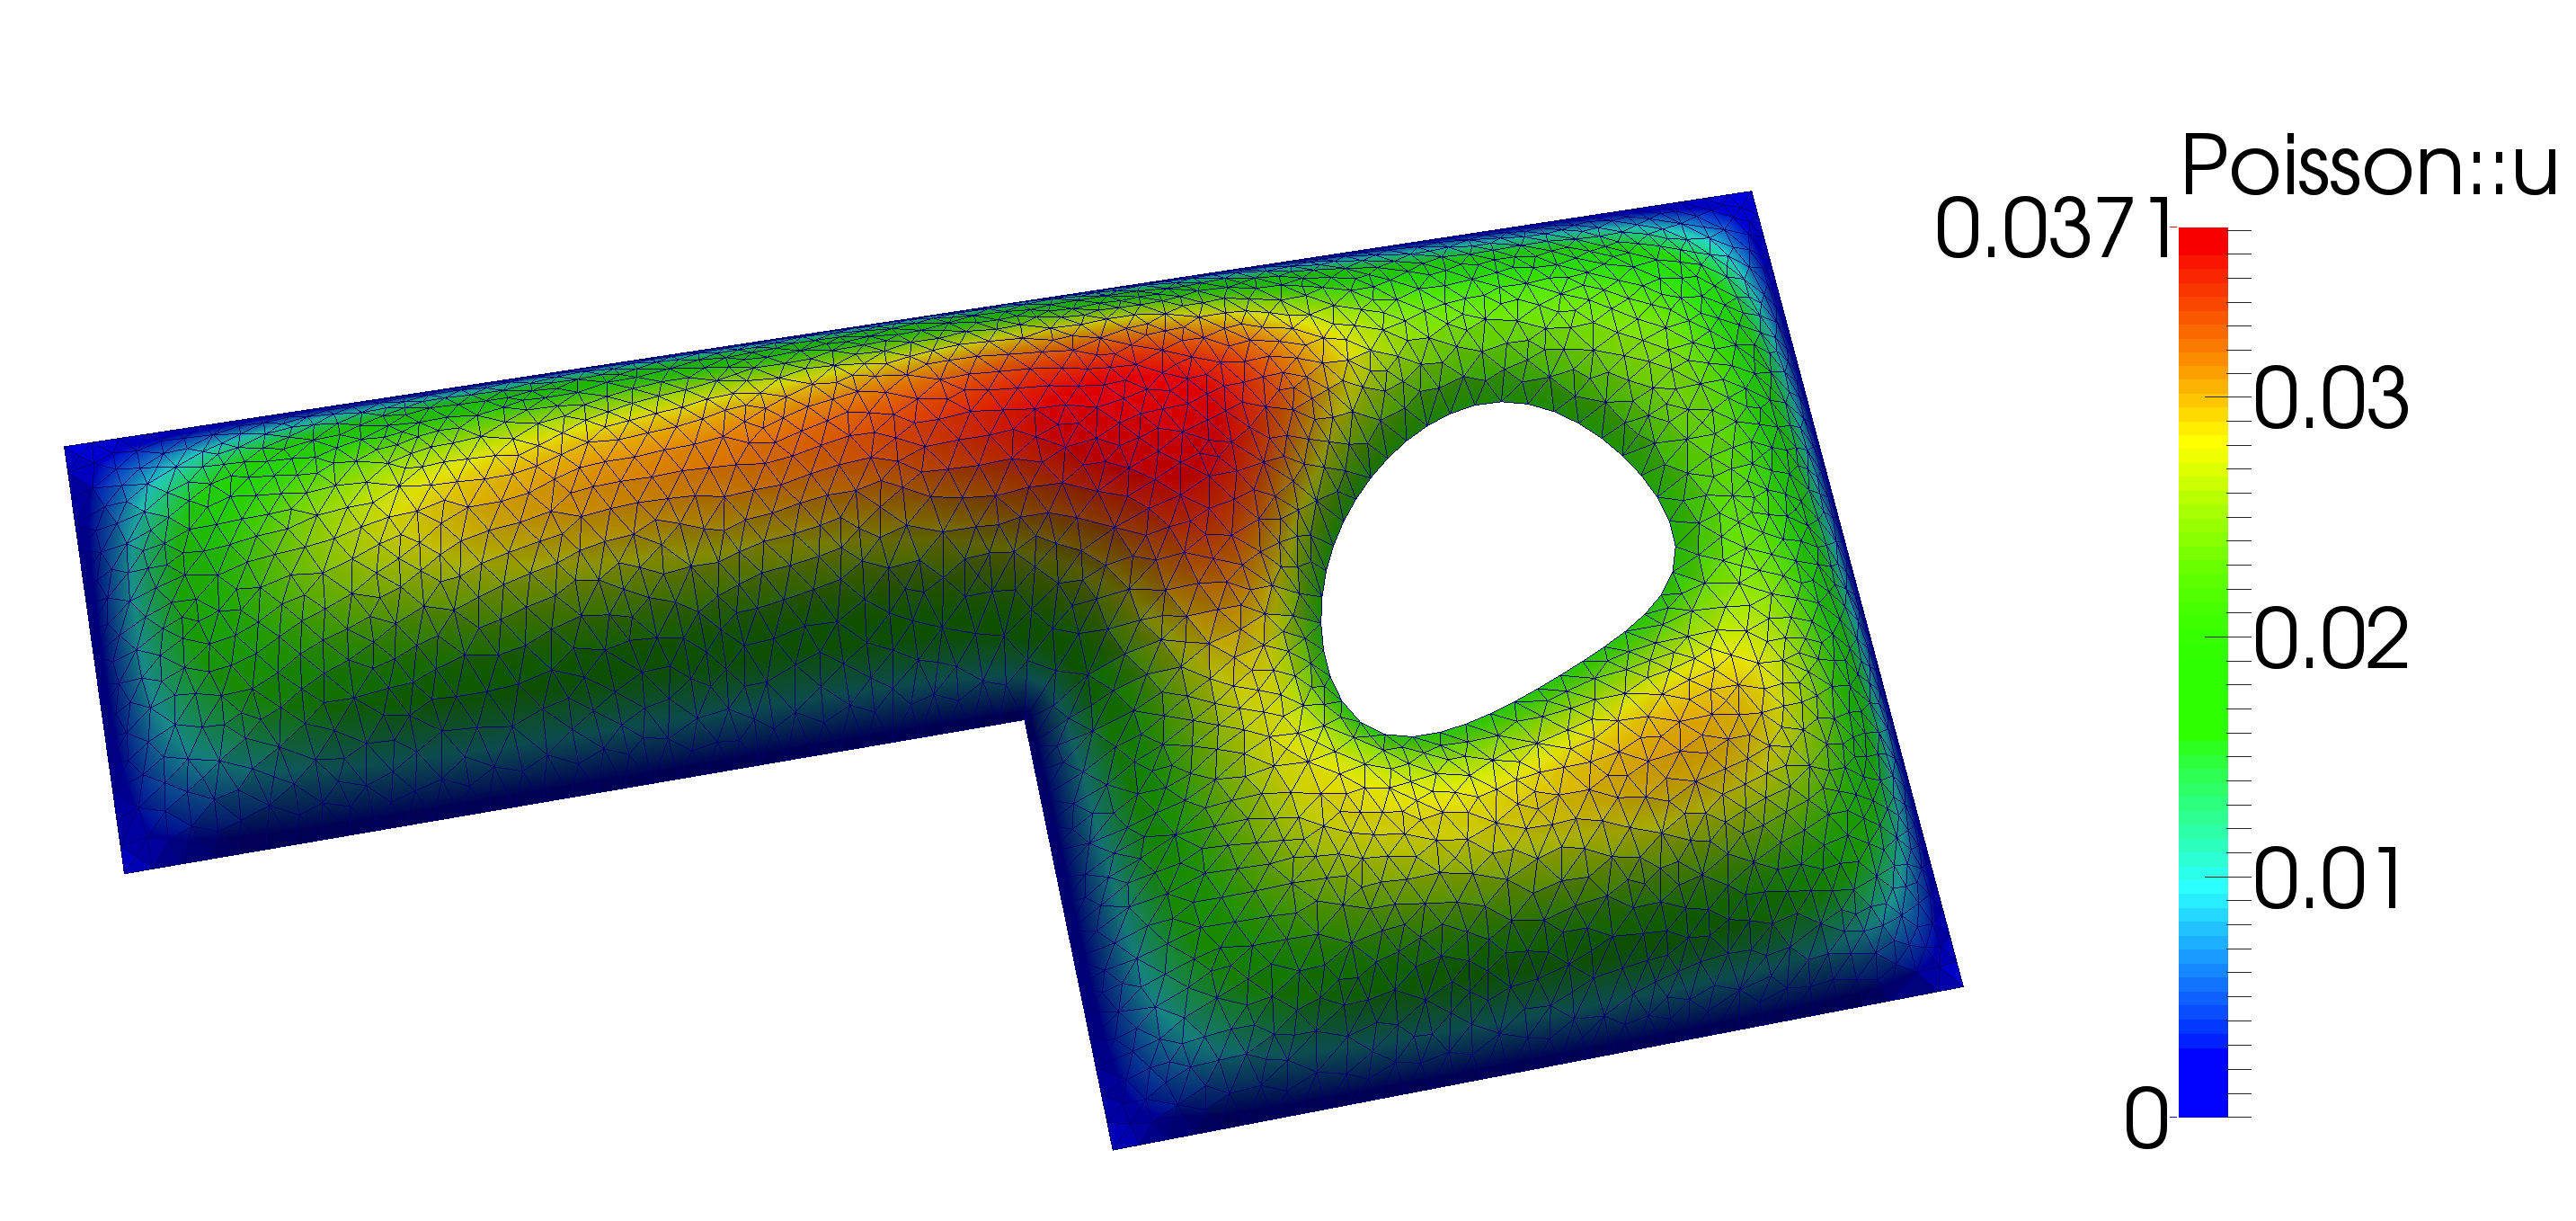
\includegraphics[width=.8\textwidth]{figures/poisson_simple_gmsh}
  \caption{\small Same problem but on an unstructured mesh generated using
    \texttt{gmsh}. Dirichlet boundary conditions for this problem are $u=0$ on
    the exterior faces and $u=0.02$ on the interior hole. }
\label{fig:poisson_gmsh}
\end{figure}

Alternatively, the mesh generation, model building and model execution
can be automated using the simulation testharness.  An example
testharness file, \texttt{poisson.shml} can be found in the gmsh
directory.  To run this file use
\begin{lstlisting}[style=Bash]
$ tfsimulationharness --test poisson.shml
\end{lstlisting}
%$
If all is successful,  the jobs will finish with
\begin{lstlisting}[style=Bash]
poisson.shml: Running tests:
poisson.shml: Running umax:
u_max = [0.037188591984999998]
poisson.shml: success.
poisson.shml: Running umin:
u_min = [0.0]
poisson.shml: success.
poisson.shml: PP
Passes:   2
Failures: 0
\end{lstlisting}


\subsubsection{Changing Elements}
\label{sec:changing-meshes}

Changing the order of an element is also trivial. For example
instead of P1 we could solve our initial problem using quadratic P2
elements by simply changing the \textbf{element} to (P2) under
\texttt{field} (i.e. Step 8).  To visualize these fields, however you
should also choose P2 as an element in
\textbf{io}$\rightarrow$\textbf{visualization}$\rightarrow$\textbf{element
(P2)}.  Changing the order of an element will force a recompile but
little else.
\begin{figure}[ht!]
  \centering
  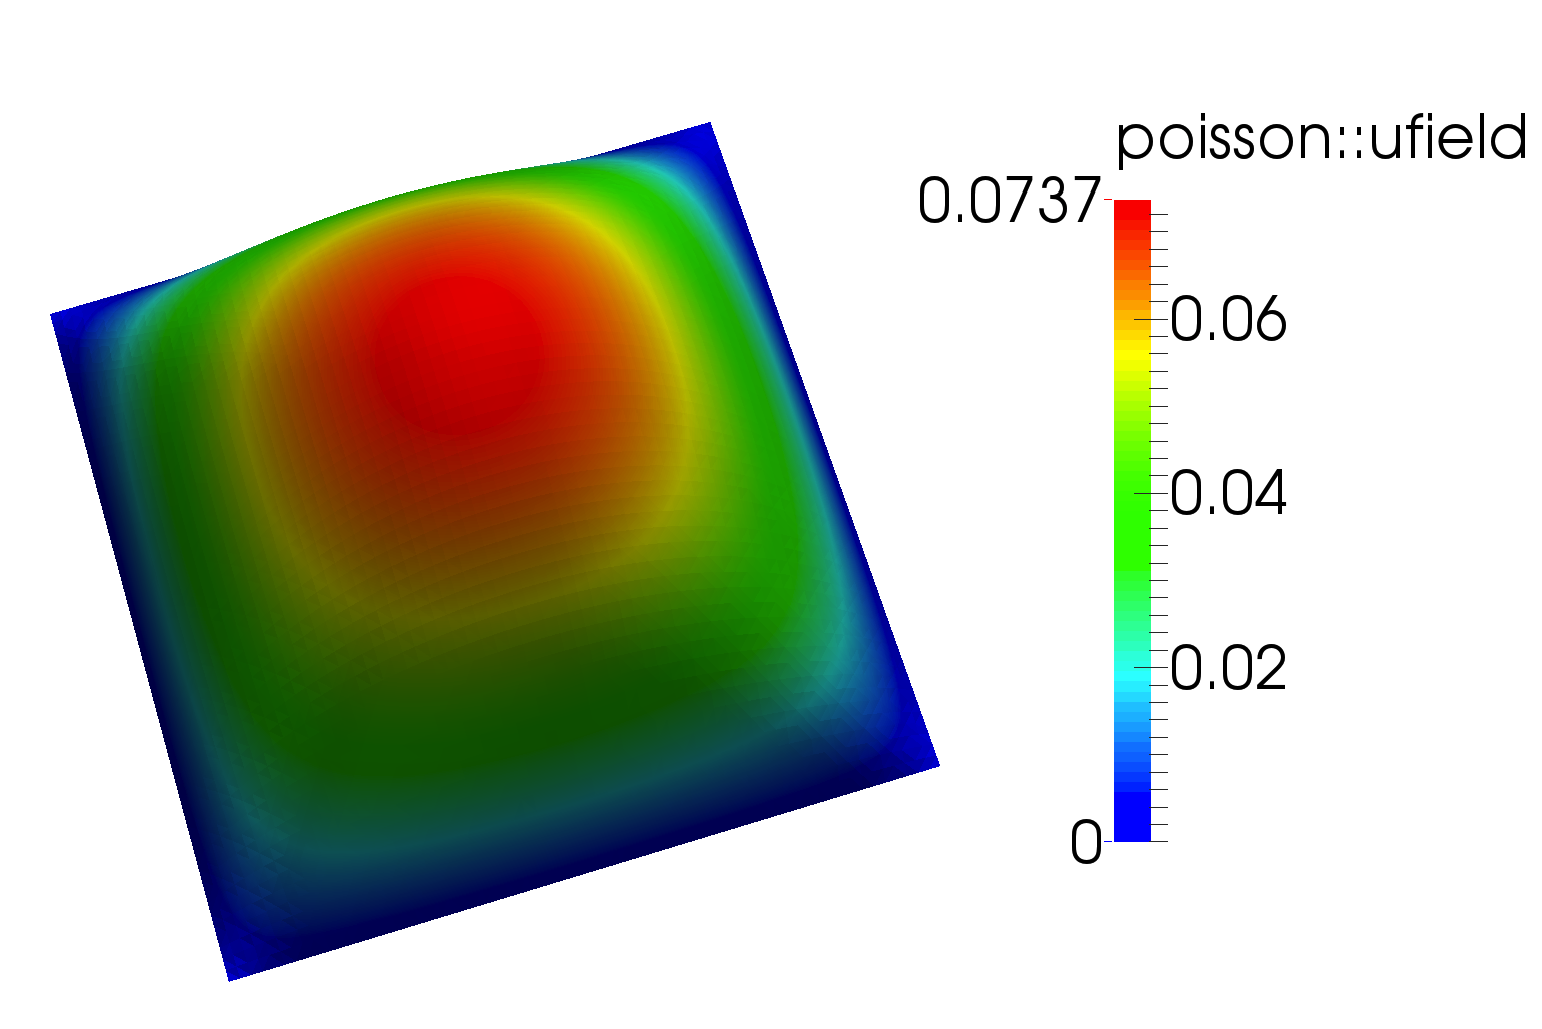
\includegraphics[width=.7\textwidth]{figures/poisson_simple_p2}
  \caption{Poisson problem with quadratic P2 elements and P2
    visualization. Compare to Figure \ref{fig:simple_poisson}}
  \label{fig:poisson-P2}
\end{figure}

To change elements entirely, for example to go with discontinuous
Galerkin (e.g. P2DG), is straightforward but forces changes to the
actual ufl for the weak form of the residual.

\subsubsection{Changing Solvers}
\label{sec:changing-solvers}

Changing solvers is straightforward as all PETSc solvers
allow choice of solvers and options at run-time.  For example, to
change from a direct solver (preonly,lu) to a algebraic-multi-grid
preconditioned conjugate gradient solver (cg,hypre) which is optimal
for poisson like problems, just edit the linear-solver to
\begin{lstlisting}[style=Bash]
iterative_method (cg)
   relative_error -> 1.e-7
   max_iterations -> 20
preconditioner (hypre)
\end{lstlisting}
If you want to exam the convergence behavior of the iterative linear
solve, simply turn on \textbf{monitors} and activate
\textbf{preconditioned\_residual}.  This will add convergence results
to the \texttt{terraferma.log-0} file which logs information about the run.
\begin{lstlisting}[style=Bash]
Solving for poisson::Solver using SNES
In FormFunction
In FormJacobian
    Residual norms for poisson_Solver_ solve.
    0 KSP Residual norm 1.249018252284e+00 
    1 KSP Residual norm 7.520968397518e-03 
    2 KSP Residual norm 1.054134570965e-04 
    3 KSP Residual norm 1.345208502264e-06 
    4 KSP Residual norm 2.609245158576e-08 
In FormFunction
Convergence for poisson::Solver
SNESConvergedReason 3
SNES n/o iterations 1
SNES n/o linear solver iterations 4
  KSPConvergedReason 2
  KSP n/o iterations 4
\end{lstlisting}
In addition, you can generate a \textbf{convergence\_file} that can be
interrogated using python scripts or provide quick visualization using
e.g.
\begin{lstlisting}[style=Bash]
$ tfplot poisson.conv
\end{lstlisting} %$
\begin{figure}[b!]
  \centering
  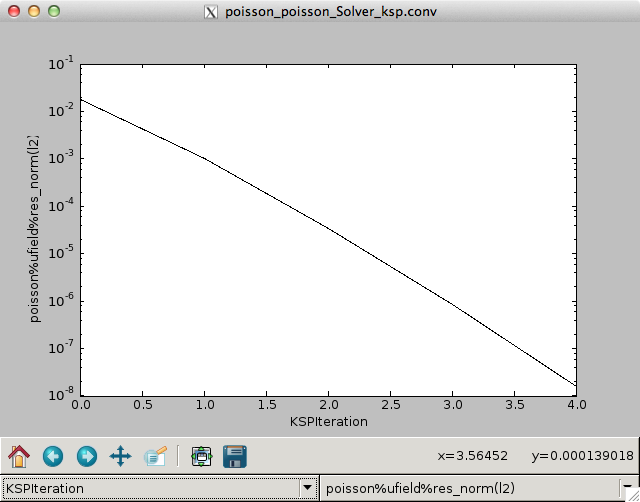
\includegraphics[width=.7\textwidth]{figures/screendumps/tfplot_cg-hypre-residuals.png}
  \caption{tfplot figure showing convergence rate of $||F||_2$ as a function of inner iteration for a (cg,hypre) iterative solver.}
  \label{fig:tfplot-convergence-poisson}
\end{figure}

{\samepage
The full \texttt{diamond} window for the linear solve should look like
\begin{center}
  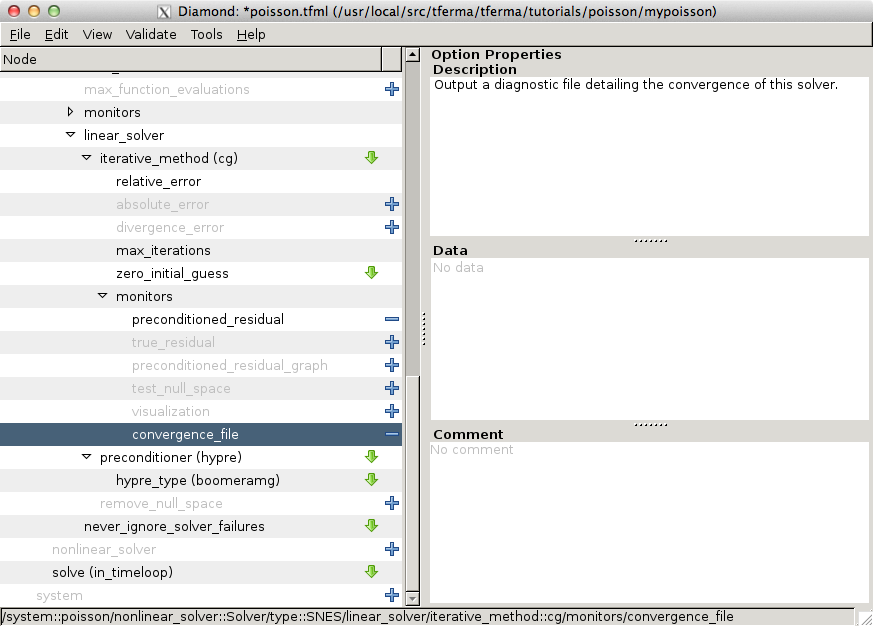
\includegraphics[width=\diamondwidth]{figures/screendumps/diamond_poisson_cg-hypre.png}
\end{center}
}

\subsubsection{Changing Dimensions}
\label{sec:changing-dimensions}

Changing dimensions is slightly more difficult, but only due to a
design issue with \texttt{diamond} which only lets you set the
dimension of the problem once.  For a basic poisson problem, it is not
difficult to simply start from scratch (or with some caution, try
editing the \texttt{.tfml} file directly). The only changes being to
\texttt{dimension} (Step 3) , \texttt{source (UnitCube)} (and
suboptions) (Step 4)  and
add additional \textbf{boundary\_ids} (Step 10).  You should also
probably change the solver to an iterative solver (e.g. (cg,hypre) or (cg,ml)) as
sparse direct solvers become significantly more expensive in memory
and time in 3-D.  A fully worked example \texttt{tfml} file can be
found in \texttt{tutorials/poisson/simple\_3d}.
Convergence behavior of the SNES and KSP is
\begin{lstlisting}[style=Bash]
Solving for Poisson::SNES using SNES
In FormFunction
  0 SNES Function norm 5.267355201652e-03 
In FormJacobian
    Residual norms for Poisson_SNES_ solve.
    0 KSP Residual norm 4.316879223510e+00 
    1 KSP Residual norm 2.742504639453e-02 
    2 KSP Residual norm 3.692535718352e-04 
    3 KSP Residual norm 4.750897104741e-06 
    4 KSP Residual norm 7.029490501627e-08 
    5 KSP Residual norm 1.289791412984e-09 
    6 KSP Residual norm 1.877399607342e-11 
In FormFunction
  1 SNES Function norm 4.727883538082e-13 
Convergence for Poisson::SNES
SNESConvergedReason 3
SNES n/o iterations 1
SNES n/o linear solver iterations 6
  KSPConvergedReason 2
  KSP n/o iterations 6
\end{lstlisting}
\begin{figure}[ht!]
  \centering
  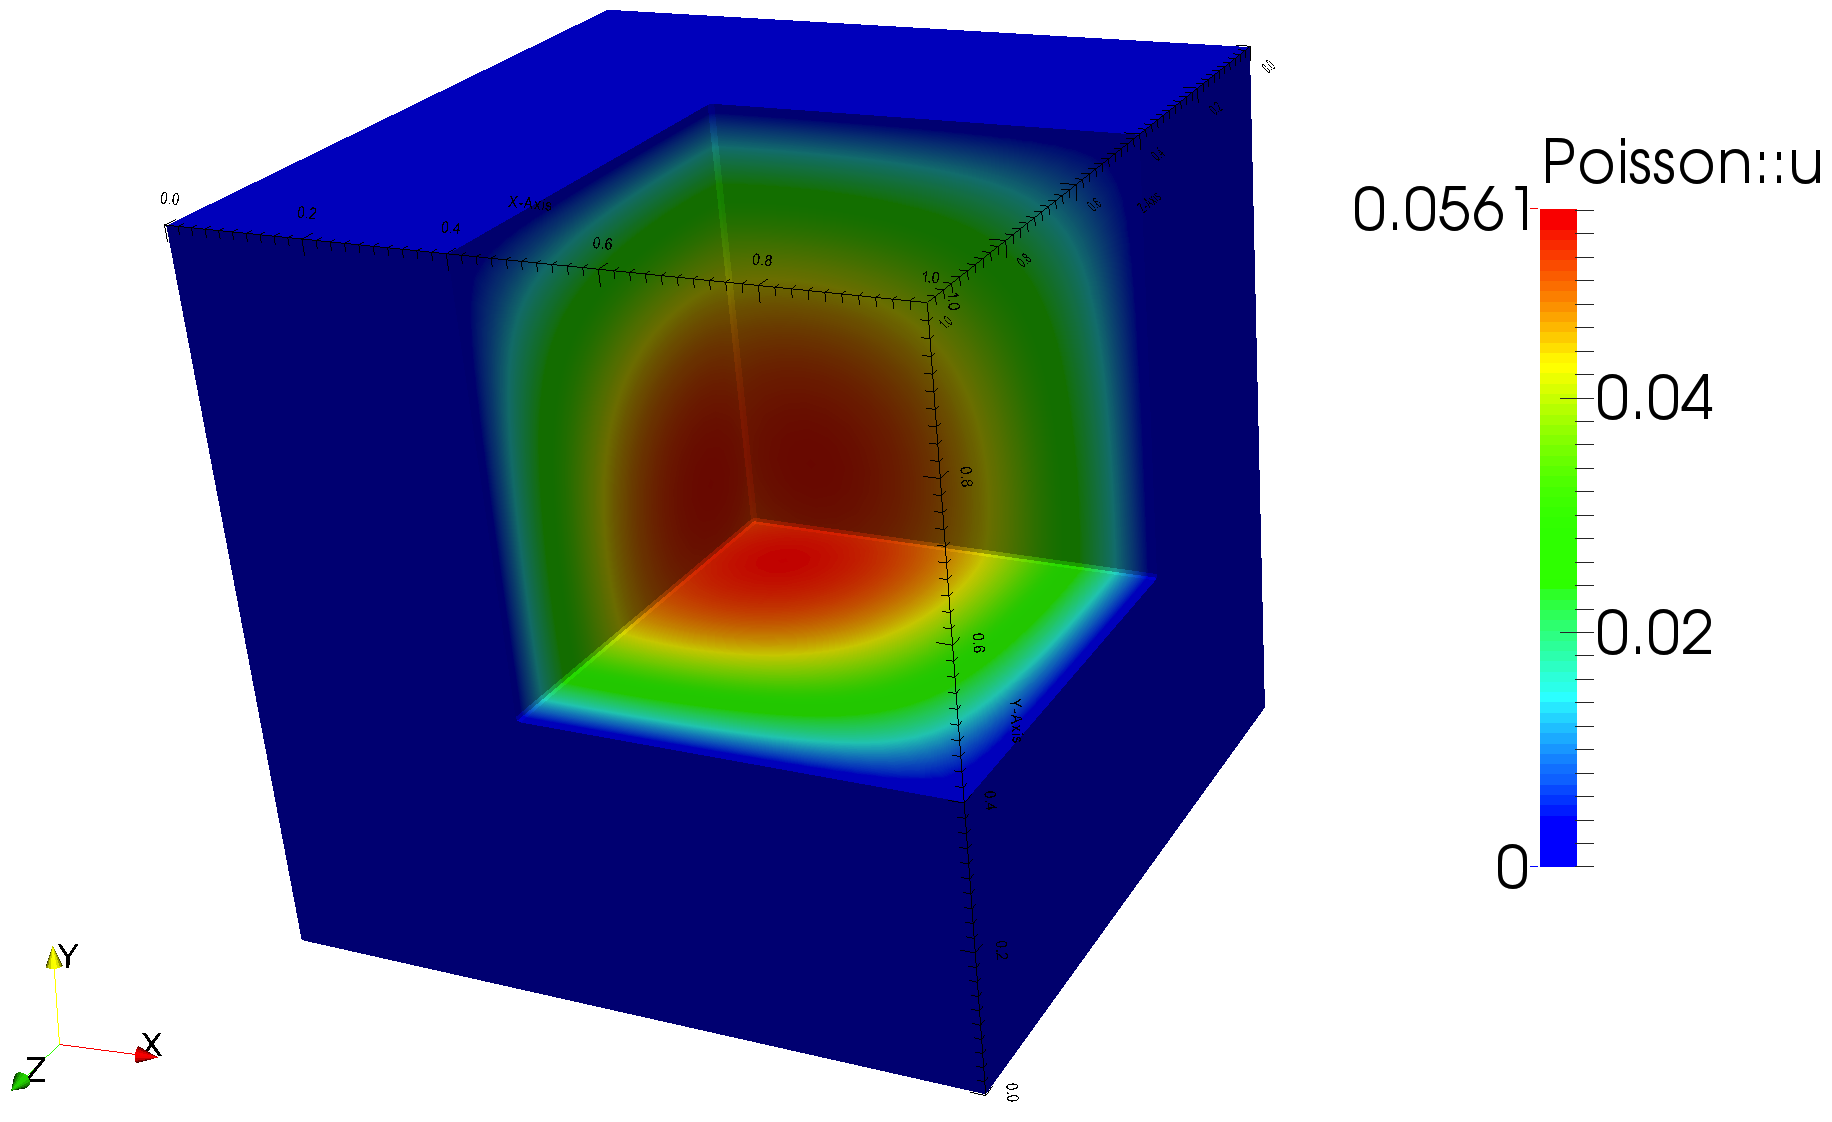
\includegraphics[width=.7\textwidth]{figures/poisson_simple_3d}
  \caption{3D poisson problem on a unit cube with unit forcing and homogeneous $u=0$ BC's}
  \label{fig:poisson-3D}
\end{figure}

\pagebreak
\subsection{Adding variable coefficients: Manufactured Solutions}
\label{sec:manuf-solut}

The basic Poisson problem with unit forcing is a useful first example,
and in fact has a (very slowly converging) spectral solution with
which we could test the accuracy of our Finite Element Model.
However, a more useful approach for testing numerical solutions is the
\emph{method of manufactured solutions}, where we simply choose a
solution $u$ and determine a forcing term $f$ and boundary conditions
that are consistent with that solution.  One particular manufactured
solution for Poisson is given in Leveque's excellent book on finite
difference methods \cite{leveque_finite_2007} which is simple (if
visually uninspiring)
\begin{equation}
  \label{eq:13}
  u_{mms}(x,y) = \exp(x + y/2)
\end{equation}
with
\begin{equation}
  \label{eq:14}
  -\nabla^{2} u_{mms} = -\frac{5}{4}\exp(x+y/2)
\end{equation}
and
\begin{equation}
  \label{eq:15}
  \grad u_{mms} = \exp(x+y/2)
  \left[
    \begin{array}{c}
 1 \\
1/2\\
\end{array}
  \right]
\end{equation}

Given the solution we can recast the problem (and now include  Neumann boundary conditions) as,
\begin{align}
  \label{eq:16}
-\nabla^2u &= f \quad\text{in } \Omega=[0,1]\times[0,1] \nonumber\\
\grad u\cdot\vec{n} & = g \quad\text{on } \partial\Omega_{N}=(x=1)\\
 u &= h \quad\text{on } \partial\Omega_{D}\nonumber
\end{align}
with  prescribed functions
\begin{align}
  \label{eq:17}
  f &= -\frac{5}{4}\exp(x+y/2)\nonumber\\
  g & = \exp(x+y/2)\\
  h &=  \exp(x+y/2)\nonumber
\end{align}
where $\partial\Omega_{N}$ are Neumann boundaries (here the right side
of the box at $x=1$) and $\partial\Omega_{D}$ are the remaining dirichlet boundaries (top, bottom,and left).

The weak form of the residual after integration by parts (and
including the surface terms) now looks like
\begin{equation}
  \label{eq:4}
  F(u_{i};u_{t}) = \int_{\Omega}
  \left(
    \grad u_{t}\cdot\grad u_{i} - u_{t}f
  \right)dx - \int_{\partial\Omega_{N}} u_{t}g ds
\end{equation}
or in ufl
\begin{lstlisting}[style=ufl]
F = (inner(grad(u_t),grad(u_i)) - u_t*f)*dx - u_t*g*ds(2)
\end{lstlisting}
where \texttt{ds(2)} implies a surface integral along boundary id 2
(right hand side for our unit square). Implementing this problem now
requires us to input variable forcing and boundary coefficients
$(f,g)$ in the form as well as impose variable Dirichlet conditions on
the other walls.

Adding variable Coefficients as FEniCS \emph{expressions} is
relatively straightforward in \TF{}. They can be included as small
python functions (which can be slow in large calculations) or as C++
expressions.  Here we will just demonstrate the python interface.  A
fully worked out example is in \texttt{tutorials/poisson/mms/poisson.tfml}.

To add these new features (and visualize the error from the analytic solution), do the following.
\begin{steps}{Step}
\item  Start with the simple poisson.tfml
  \begin{lstlisting}[style=Bash]
$ mkdir mymms
$ cd mymms
$ cp $TF_HOME/share/terraferma/tutorials/poisson/simple/poisson.tfml .    
  \end{lstlisting}
\item Change the coefficient \texttt{f} in \textbf{system (Poisson)} to a python Expression. Unfold the \textbf{coefficient (f)} tab until you see the Expression value as \textbf{constant}. 
\begin{center}
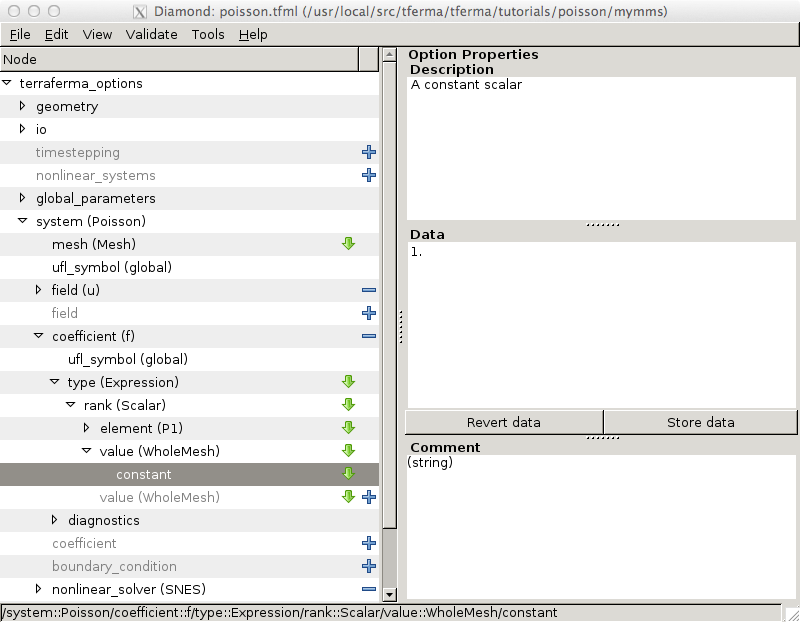
\includegraphics[width=\diamondwidth]{figures/screendumps/diamond_poisson_f_value.png}
  \end{center}
\item using the drop down menu, change the value from \textbf{constant} to \textbf{python} and in the data window, replace \texttt{(string)} with the following small python function
  \begin{lstlisting}[style=python]
from math import exp
def val(x):
  global exp
  return -5./4.*exp(x[0] + x[1]/2.)   
  \end{lstlisting}
(and be careful about the indentation). \texttt{f} is now a variable coefficient which will return $f(\vec{x}) = -5/4(\exp(x + y/2)$ at any point $\vec{x}$. Your diamond window should now look like
\begin{center}
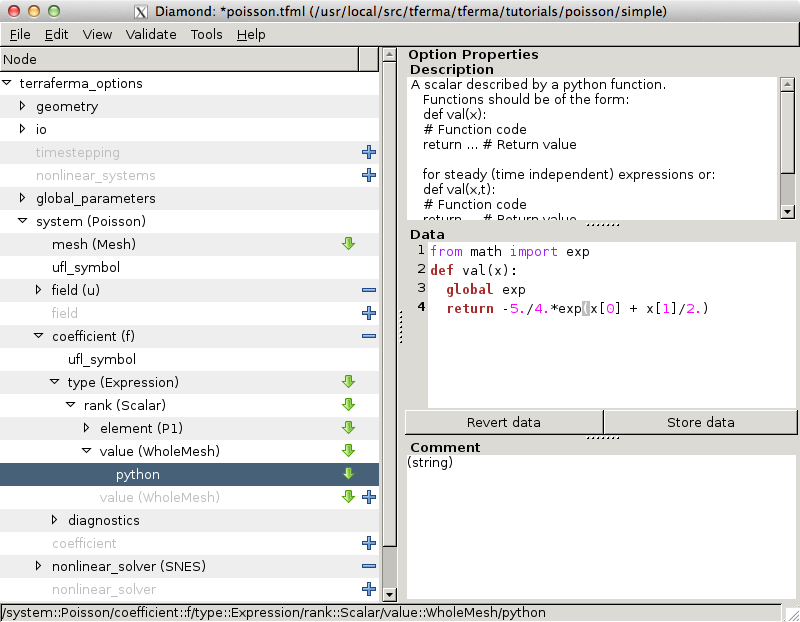
\includegraphics[width=\diamondwidth]{figures/screendumps/diamond_poisson_mms_f_value.png}
  \end{center}
\item \textbf{Change the Dirichlet Boundary conditions}.  Under \textbf{field (u)}$\rightarrow$\textbf{type (Function)}, find and unfold the \textbf{boundary\_condition (homogeneous)} tab.  Select \textbf{boundary\_ids} and remove \texttt{2} (right boundary) from the list to leave \texttt{1 3 4}.  Then unfold \textbf{sub\_components (All)}$\rightarrow$\textbf{type (Dirichlet)} and change the value from \textbf{constant} to \textbf{python} and add the python function
\begin{lstlisting}[style=python]
from math import exp
def val(x):
  global exp
  return exp(x[0] + x[1]/2.)    
\end{lstlisting}
\begin{center}
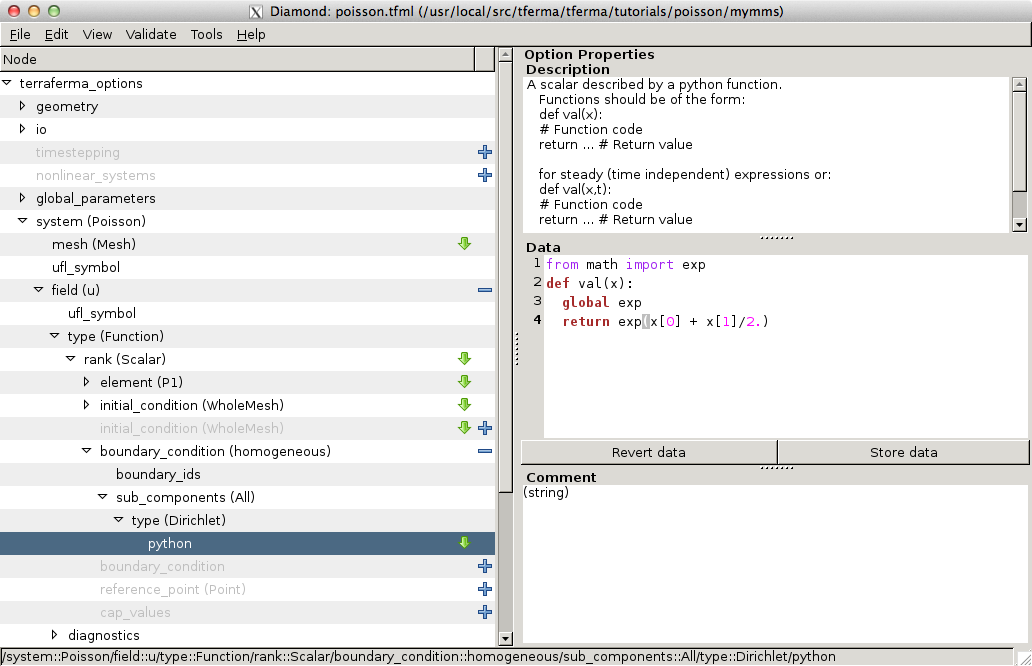
\includegraphics[width=\diamondwidth]{figures/screendumps/diamond_poisson_mms_bcs.png}
  \end{center}
\item \textbf{Add a new coefficient (g)} for the Neumann boundary conditions.  The cleanest way to do this is to activate a new coefficient tab and set the \texttt{name} and \textbf{ufl\_symbol} to \texttt{g},  the \textbf{element} to \texttt{P1} and the \textbf{value (WholeMesh)} to \textbf{python} and add the python function
\begin{lstlisting}[style=python]
from math import exp
def val(x):
  global exp
  return exp(x[0] + x[1]/2.)    
\end{lstlisting}

The slightly dangerous, but quicker way is to use the copy and paste features of \texttt{diamond} where you can copy and paste entire sub-trees of options, i.e. select the top tab \texttt{coefficient (f)}, and using the edit menu select \texttt{Copy}, then activate a new coefficient tab and select \texttt{Paste}.  This should give you a copy of the entire options tree of the \textbf{coefficient (f)}.  You now just have to edit the coefficient \texttt{name} and \textbf{ufl\_symbol} to \texttt{g}, and edit the \textbf{python} function to the listing above. 
 \begin{center}
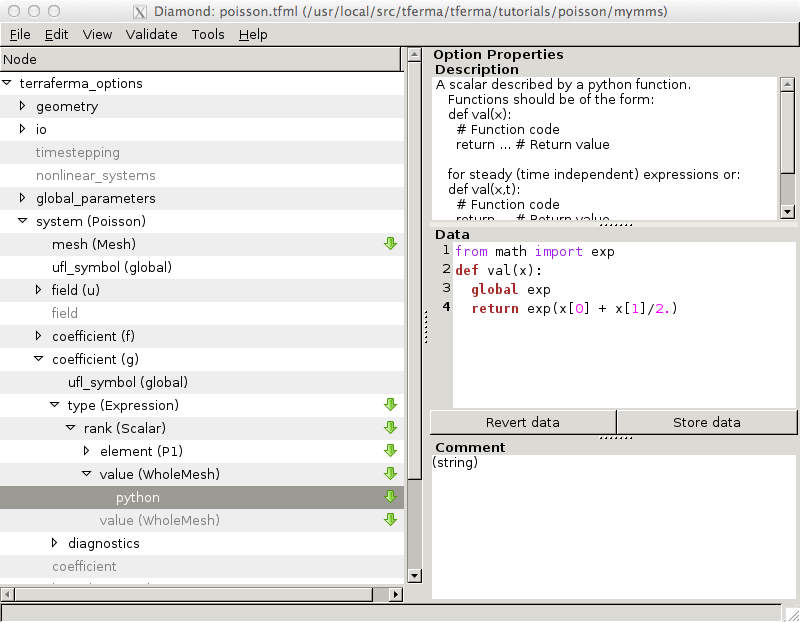
\includegraphics[width=\diamondwidth]{figures/screendumps/diamond_poisson_mms_g_value.png}
  \end{center} 
\item \textbf{Edit the UFL for the residual}. We now have to add the boundary terms for \texttt{g} into the residual equations.  Unfold \textbf{nonlinear\_solver (SNES)}$\rightarrow$\textbf{type (SNES)} and choose \textbf{form (Residual)}, and change
  \begin{lstlisting}[style=UFL]
    F = (inner(grad(u_t),grad(u_i)) - u_t*f)*dx
  \end{lstlisting}
to
  \begin{lstlisting}[style=UFL]
    F = (inner(grad(u_t),grad(u_i)) - u_t*f)*dx - u_t*g*ds(2)
  \end{lstlisting}
\begin{center}
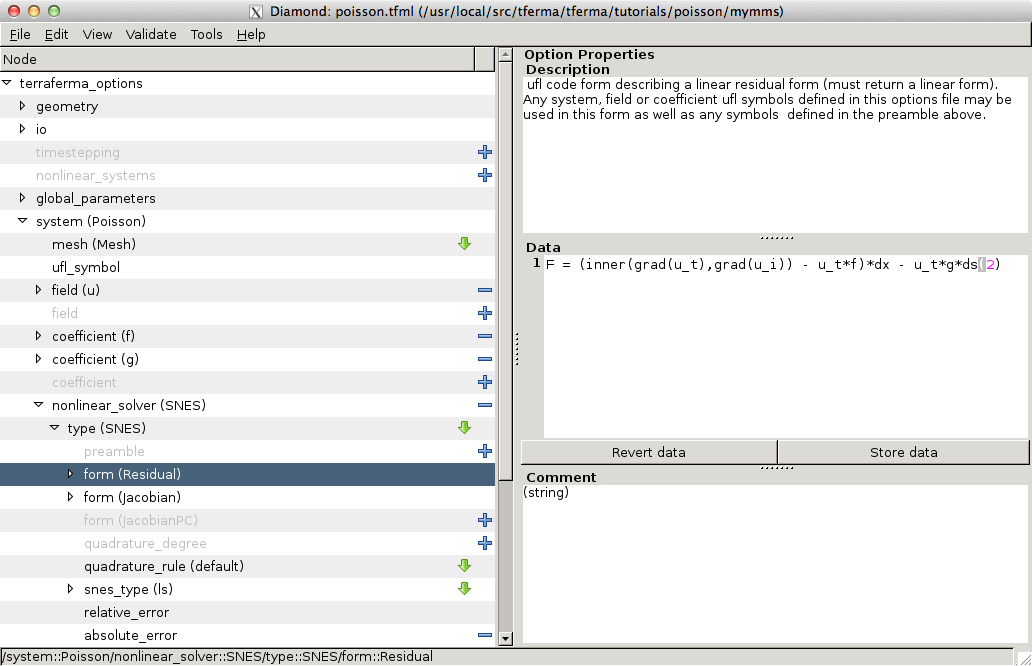
\includegraphics[width=\diamondwidth]{figures/screendumps/diamond_poisson_mms_residual.png}
  \end{center}
\item At this point you should be able to build and run the new model
  \begin{lstlisting}[style=Bash]
$ tfbuild poisson.tfml
$ cd build
$ make run
   \end{lstlisting} %$
and it should look something like
\begin{figure}[h]
  \centering
  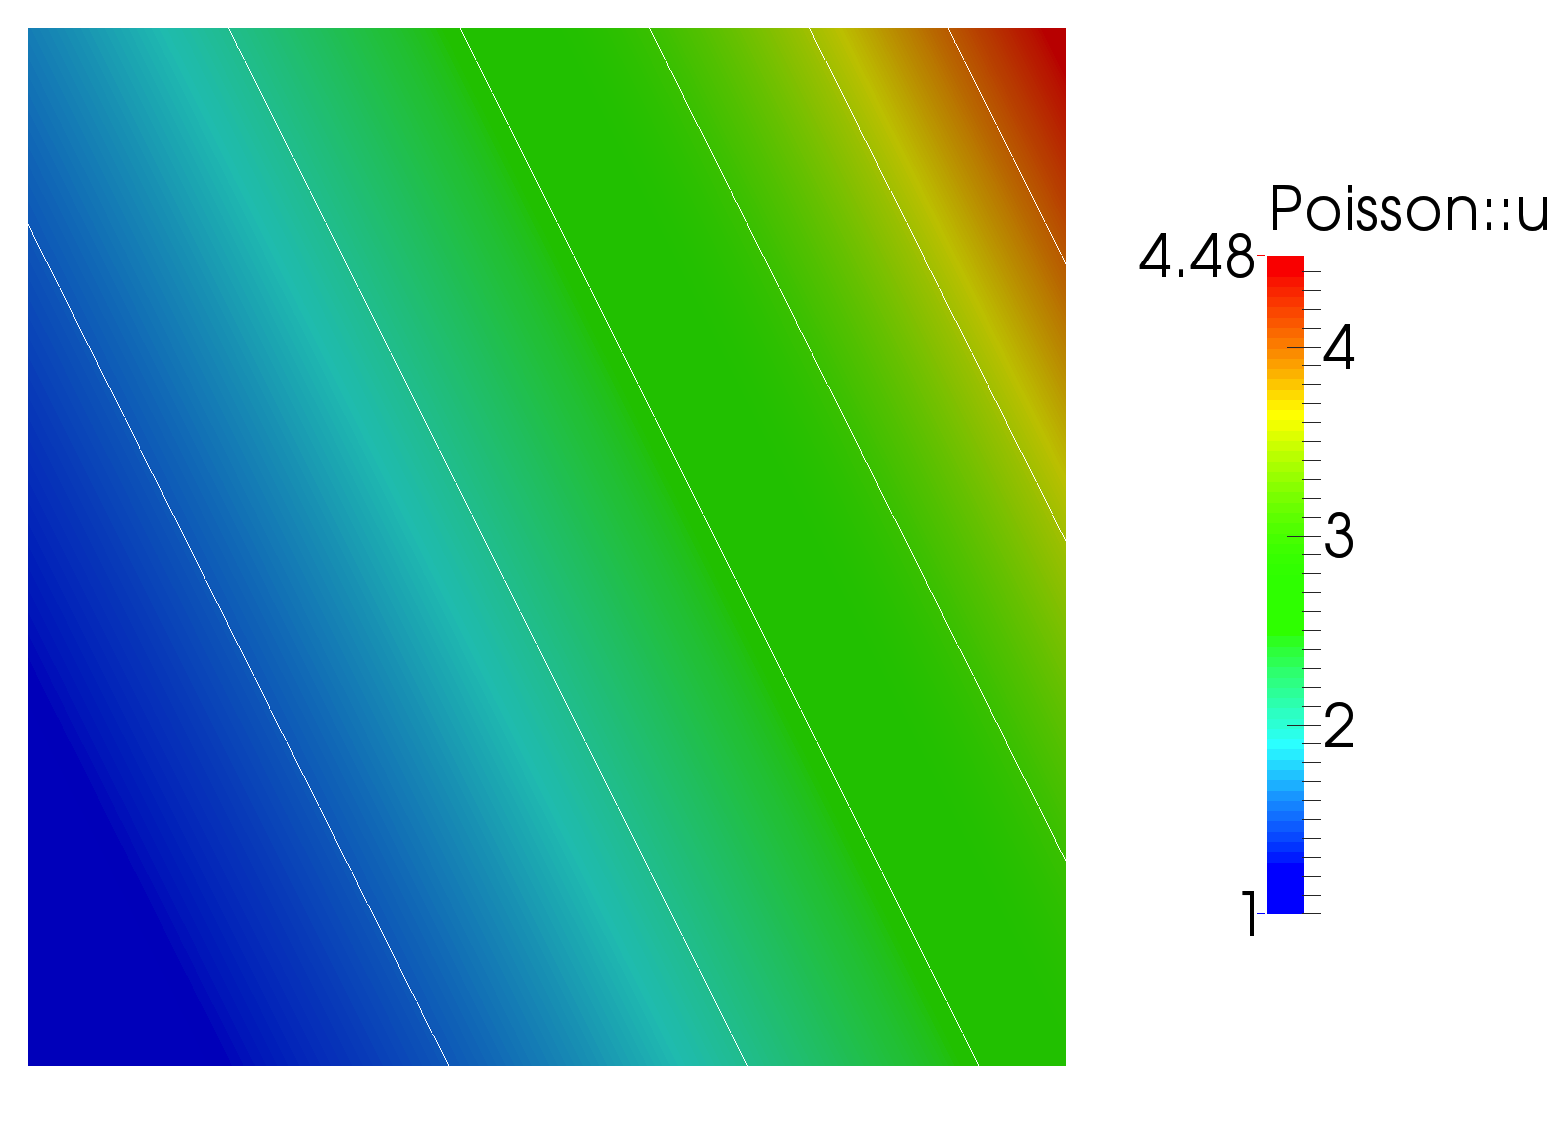
\includegraphics[width=.7\textwidth]{figures/poisson_mms.png}
  \caption{solution for the Poisson mms example (not terribly exciting looking)}
  \label{fig:poisson_mms}
\end{figure}

\end{steps}

\paragraph{Adding Error monitoring}
\label{sec:adding-error-monit}

Pretty pictures are nice,  but the whole point of MMS is that we can
calculate the exact error to test our solutions as well as
convergence.  The example program
\texttt{\$TF\_HOME/share/terraferma/tutorials/poisson/mms/poisson.tfml} has two
mechanisms for calculating and monitoring the absolute error of this
solution.  One simple approach is just to  visualize errors by
creating a new system that calculates the projection of $e = u -
u_{exact}$ onto the Function Space P1 and outputting this solution for
visualization.  The example \texttt{poisson.tfml} includes this
additional system.

An alternate approach, however is to calculate a functional
\begin{equation}
  \label{eq:18}
  e^{2} = \int_{\Omega} (u-u_{exact})^{2} dx
\end{equation}
which is the square of the L2 norm of the absolute error and output it
to statistics for later processing.  To implement this
\begin{steps}{Step}
\item First create another coefficient by copying \textbf{coefficient (g)} then changing the name to \texttt{AnalyticSolution} and \textbf{ufl\_symbol} to \texttt{ue}.  The python to evaluate \texttt{g} and the analytic solution are the same (coincidentally).
\item \textbf{Add a functional to the system} Next we have to attach a
  functional to the system  and output to statistics.  Do the following
  \begin{steps}{step}
  \item activate the greyed out tab \textbf{functional} and give it a \textbf{name} (L2NormErrorSquared) and a piece of ufl to evaluate the functional in Eq.\ (\ref{eq:18})
    \begin{lstlisting}[style=UFL]
e2 = ( u - ue )**2 *dx
    \end{lstlisting}
  \item set the  \textbf{ufl\_symbol} for the functional to \texttt{e2}
  \end{steps}
\end{steps}
\begin{center}
    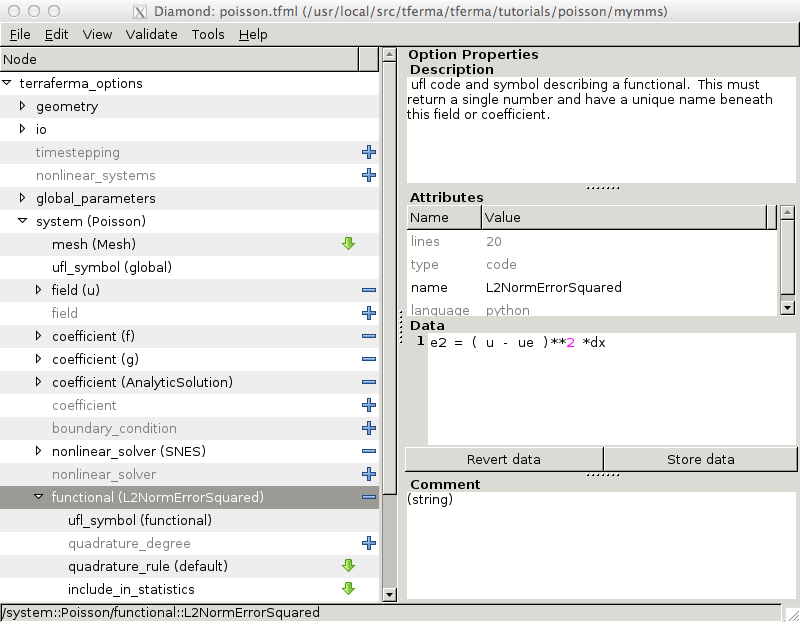
\includegraphics[width=\diamondwidth]{figures/screendumps/diamond_poisson_mms_functional.png}
\end{center}
The value of the functional will now be written to the statistics file
\texttt{poisson.stat} as part of a python dictionary that can be
either viewed with \texttt{tfplot} or interrogated using additional
python modules furnished with \TF{}.

\paragraph{Running parameter sweeps using the simulation test-harness}
\label{sec:runn-param-sweeps}

To calculate convergence for this mms problem requires running our
basic \texttt{.tfml} file for a range of mesh sizes, accumulating the
errors for each mesh file and producing output (e.g. a convergence
plot such as Figure \ref{fig:poisson_convergence} ).  To aid in
running multiple simulations or parameter sweeps as well as providing
a uniform testing environment for regression testing of \TF,  we have
also developed the \emph{TerraFERMA simulation test-harness}. 

While an individual \texttt{.tfml} file records all the options
required for a single instance of a model, a test harness options file
(with extension
\texttt{.shml}  for simulation harness markup language), controls the
work flow for building, running and testing multiple models as well as
handling dependencies such as mesh generation.   We have included an example in
\texttt{\$TF\_HOME/share/terraferma/tutorials/poisson/mms/poisson.shml},
that takes as input  the tfml file \texttt{poisson.tfml}  and runs a
parameter sweep over the mesh parameter \texttt{ncells}, but using the
python bindings to the spud library (libspud) to generate a directory
structure and a set of individual \texttt{tfml} files for each model.
In addition,  the test harness will build a single copy of the binary,
run multiple versions of the model,  collect error information for
each grid spacing and plot the convergence behavior.  It will also
provide a test to make sure that the  MMS problem show the expected
quadratic convergence.

To view the testharness file use
\begin{lstlisting}[style=Bash]
 $ diamond poisson.shml
\end{lstlisting} %$
To run it, we use the utility function
\texttt{tfsimulationharness}.  Options for tfsimulationharness are
provided using 
\begin{lstlisting}[style=Bash]
$ tfsimulationharness -h
\end{lstlisting} %$
% usage: tfsimulationharness [-h] [-n NTHREADS] [-r [depth]] [-l length [length ...]] [-p parallelism] [-o ownerid [ownerid ...]] [-t tag [tag ...]] [-e tag [tag ...]] [--generate] [--configure] [--build] [--run] [--test]
%                            [--just-test] [--just-list] [--list-input] [--clean] [-f]
%                            filename [filename ...]
%
% Run simulations and manipulate the output data.
%
% positional arguments:
%   filename              specify filename(s)
%
% optional arguments:
%   -h, --help            show this help message and exit
%   -n NTHREADS, --nthreads NTHREADS
%                         number of threads
%   -r [depth], --recursive [depth]
%                         recursively search the directory tree for files (if no depth is specified full recursion will be used)
%   -l length [length ...], --length length [length ...]
%                         length(s) of problem (if unspecified will run all lengths)
%   -p parallelism, --parallelism parallelism
%                         parallelism of problem: options are serial, parallel or any (default=any)
%   -o ownerid [ownerid ...], --owner ownerid [ownerid ...]
%                         run only tests that have specific owner ids (if unspecified will include all owners)
%   -t tag [tag ...], --tags tag [tag ...]
%                         run only tests that have specific tags (if unspecified will run all tags)
%   -e tag [tag ...], --exclude tag [tag ...]
%                         run only tests that do not have specific tags (takes precedence over -t, if unspecified will not exclude any tags)
%   --generate            generate the simulation directories and input
%   --configure           configure the simulations
%   --build               build the simulations
%   --run                 run the simulations
%   --test                test the simulations
%   --just-test           only test the current output of the simulations (do not rerun)
%   --just-list           only list the simulations
%   --list-input          list the input to the simulations
%   --clean               removes the run (and build) directories from previous simulation runs
%   -f, --force           force rebuild(s)
% \end{lstlisting} %$
which provides considerable flexibility in building, running and
testing specific applications. %  The testharness is currently
% undocumented (but needs to be added as an appendix to this document or
% on the wiki).

To build, run and test the example mms problem just
\begin{lstlisting}[style=Bash]
$ cd mms
$ tfsimulationharness --test poisson.shml
\end{lstlisting} %$
which will generate two directory structures:
\texttt{poisson.tfml.build} contains the binary file and
\texttt{poisson.tfml.run} contains a set of subdirectories for each
individual run labeled by the parameter (in this case
\texttt{ncells\_8}, \texttt{ncells\_16}, etc.).   Using the
\texttt{--test} option, it will also calculate the best-fit degree of
accuracy (which should be $p=2$ for a second order accurate problem in
$P_1$) and check that it is greater than 1.9.  It will also use
matplotlib to produce the pdf file shown in  Figure
\ref{fig:poisson_convergence}.

Output of a successful run should look like
\begin{lstlisting}[style=Bash]
poisson.shml: Running tests:
poisson.shml: Running error_l2_p1:
OrderedDict([('ncells', ['8', '16', '32', '64', '128'])])
***********  order of accuracy p= 1.98737547825
***********  convergence figure in poisson_convergence.pdf
poisson.shml: success.
poisson.shml: P
Passes:   1
Failures: 0
\end{lstlisting}

\begin{figure}[ht!]
  \centering
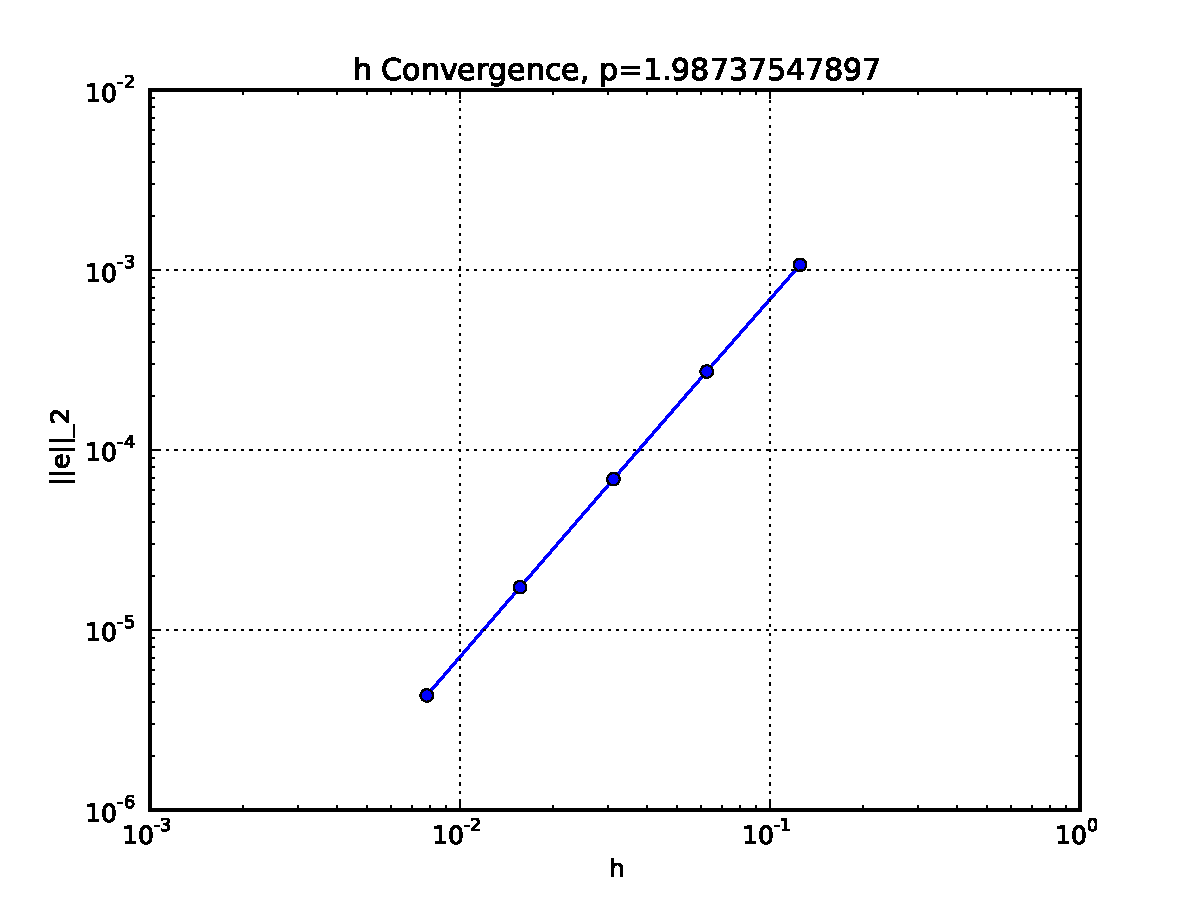
\includegraphics[width=.6\textwidth]{figures/poisson_convergence.pdf}
  \caption{Convergence plot for poisson mms problem. $h=1/N$ is the nominal grid spacing}
  \label{fig:poisson_convergence}
\end{figure}






%%% Local Variables: 
%%% mode: latex
%%% TeX-master: "tftutorials"
%%% End: 

\chapter{Stokes Equation}
\label{cha:stokes-equation}

\section{Problem Overview}
\label{sec:problem-formulation}

A fundamental problem in Solid Earth Sciences is the solution of
Stokes equation for the incompressible creeping flow of a highly
viscous fluid.
\begin{align}
-\div\eta(\grad\vec{v} + \grad\vec{v}^{T}) + \grad p &= \vec{f}\\ 
\div \vec{v} = 0 & 
\end{align}
where $\vec{v}$ is the fluid velocity field,  $p$ is the pressure
which acts to enforce the incompressibility constraint, $\eta$ is the
fluid viscosity and $\vec{f}$ are body forces (usually buoyancy) that
drive flow.

Stokes Equation is computationally and mathematically more challenging
to solve than Poisson's equation in Chapter
\ref{cha:poiss-equat-unit}, particularly for non-constant viscosity.
To begin with, Stokes is a coupled system of PDE's for $\vec{u} =
(\vec{v},p)$ which in finite elements we can capture by describing
$\vec{u}$ as a mixed-element on a mixed finite element function space.
The proper choice of elements for $\vec{v}$ and $p$ is critical for
stability and solution of this problem.  Elman et
al. \cite{elman_finite_2005} provide a good discussion of the issues
for the isoviscous case and May and Moresi \cite{may_preconditioned_2008} provides
important extensions and tests of a large range of iterative solvers
for the variable viscosity case.

Here we will just illustrate the basic isoviscous problem with a range
of direct and iterative solvers that highlight the Fieldsplit block
preconditioners in PETSc \cite{brown_composable_2012} and their
implementation in \TF{}.  While the computational choices required to
solve Stokes efficiently and accurately are more involved
than Poisson,  we will demonstrate that setting the problem up in
\TF{} is a straightforward extension of the problems in Chapter
\ref{cha:poiss-equat-unit}. 

\subsection{Variational forms}
\label{sec:variational-forms}

For this tutorial, we will use a stable ``Taylor-Hood'' element where
velocity is assumed to be a vector valued function with each component
a piecewise quadratic function (i.e.\ for a 2-D problem on triangles
$\vec{v}\in [P_{2}\times P_{2}]$) while the pressure is piecewise
linear ($p\in P_{1}$) such that the entire system $\vec{u}\in \fspace
= [[P_{2}\times P_{2}]\times P_{1}]$.  The variational form of the
(possibly) non-linear problem can be written
\begin{quote}
  \fbox{\parbox{.9\textwidth}{Find $\vec{u}\in \fspace$ such that
      \begin{equation}
         F(\vec{u};\vec{u}_{t}) =0 
      \end{equation}
  for all test functions $\vec{u}_{t}=(\vec{v}_{t},p_{t}) \in\fspace$.}}
\end{quote}
 where $F(\vec{u};\vec{u}_{t}) = F_{\vec{v}} + F_{p}$ with
\begin{align}
         F_{\vec{v}} =  & \int_\Omega \left[\dot{\epsilon}(\vec{v}_{t}):
             2\eta \dot{\epsilon}(\vec{v}_{i}) -
             p_{i}\div\vec{v}_t  - \vec{v}_{t} \cdot\vec{f} \right]d\vec{x}  \\
 F_{p} =& -\int_\Omega p_t\div\vec{v}_{i} d\vec{x}
\end{align}
(after some algebra and integration by parts). $F_{\vec{v}}$ is the
velocity residual, $F_{p}$ is the pressure residual, but our solution
is minimizing residual of the entire system.  Here
\begin{equation}
  \label{eq:19}
  \dot{\epsilon}(\vec{v}) = \frac{1}{2}
  \left(
\grad\vec{v} + \grad\vec{v}^{T}
  \right)
\end{equation} is the strain-rate tensor (i.e. the symmetric part of
deformation tensor $\grad\vec{v}$).   

The weak form of the residual in UFL looks quite similar
\begin{lstlisting}[style=UFL]
Fv = (inner(sym(grad(v_t)),2.*eta*sym(grad(v_i)))
    - p_i*div(v_t) - inner(v_t,f)*dx  
Fp = -p_t*div(v_i)*dx 

F =  Fv + Fp 
\end{lstlisting}
and the Jacobian
\begin{lstlisting}[style=UFL]
  J = derivative(F,u_i,u_a)
\end{lstlisting}
assembles into the $2\times2$ block system
\begin{equation}
  \label{eq:20}
  J =
  \left[
    \begin{array}{cc}
      K & G \\
      G^{T} & 0\\
    \end{array}
  \right]
\end{equation}

The discrete problem Eq. (\ref{eq:20}),  is the classic Stokes
saddle-point system.  Here we will just scratch the
surface with a simplified MMS solution that implements some basic solution
strategies taken from \cite{elman_finite_2005}.  To fully specify the
problem we need boundary conditions and a forcing function $\vec{f}$. Elman et. al \cite{elman_finite_2005} provide  the
2-D manufactured solution 
\begin{align}
  \vec{v}_{x}(x,y) =& 20xy^{3} \nonumber \\
  \vec{v}_{y}(x,y) =& 5(x^{4} - y^{4})  \label{eq:stokes-mms}
\\
   p(x,y) =& 60x^{2}y - 20y^{3} \nonumber \\
   \vec{f}(x,y) =& \vec{0} \nonumber 
\end{align}
on the domain  $\Omega=[-1,1]\times[-1,1]$ with Dirichlet boundary conditions on velocity interpolated from the
analytic solution.  Note: the discrete problem with all Dirichlet
conditions on velocity is singular (with a trivial constant null space
for the pressure) and some care needs to be taken with both direct and
iterative solvers to solve this problem accurately. Figure
\ref{fig:stokesMMS} shows a \TF{} solution for this problem.

\begin{figure}[htbp!]
  \centering
  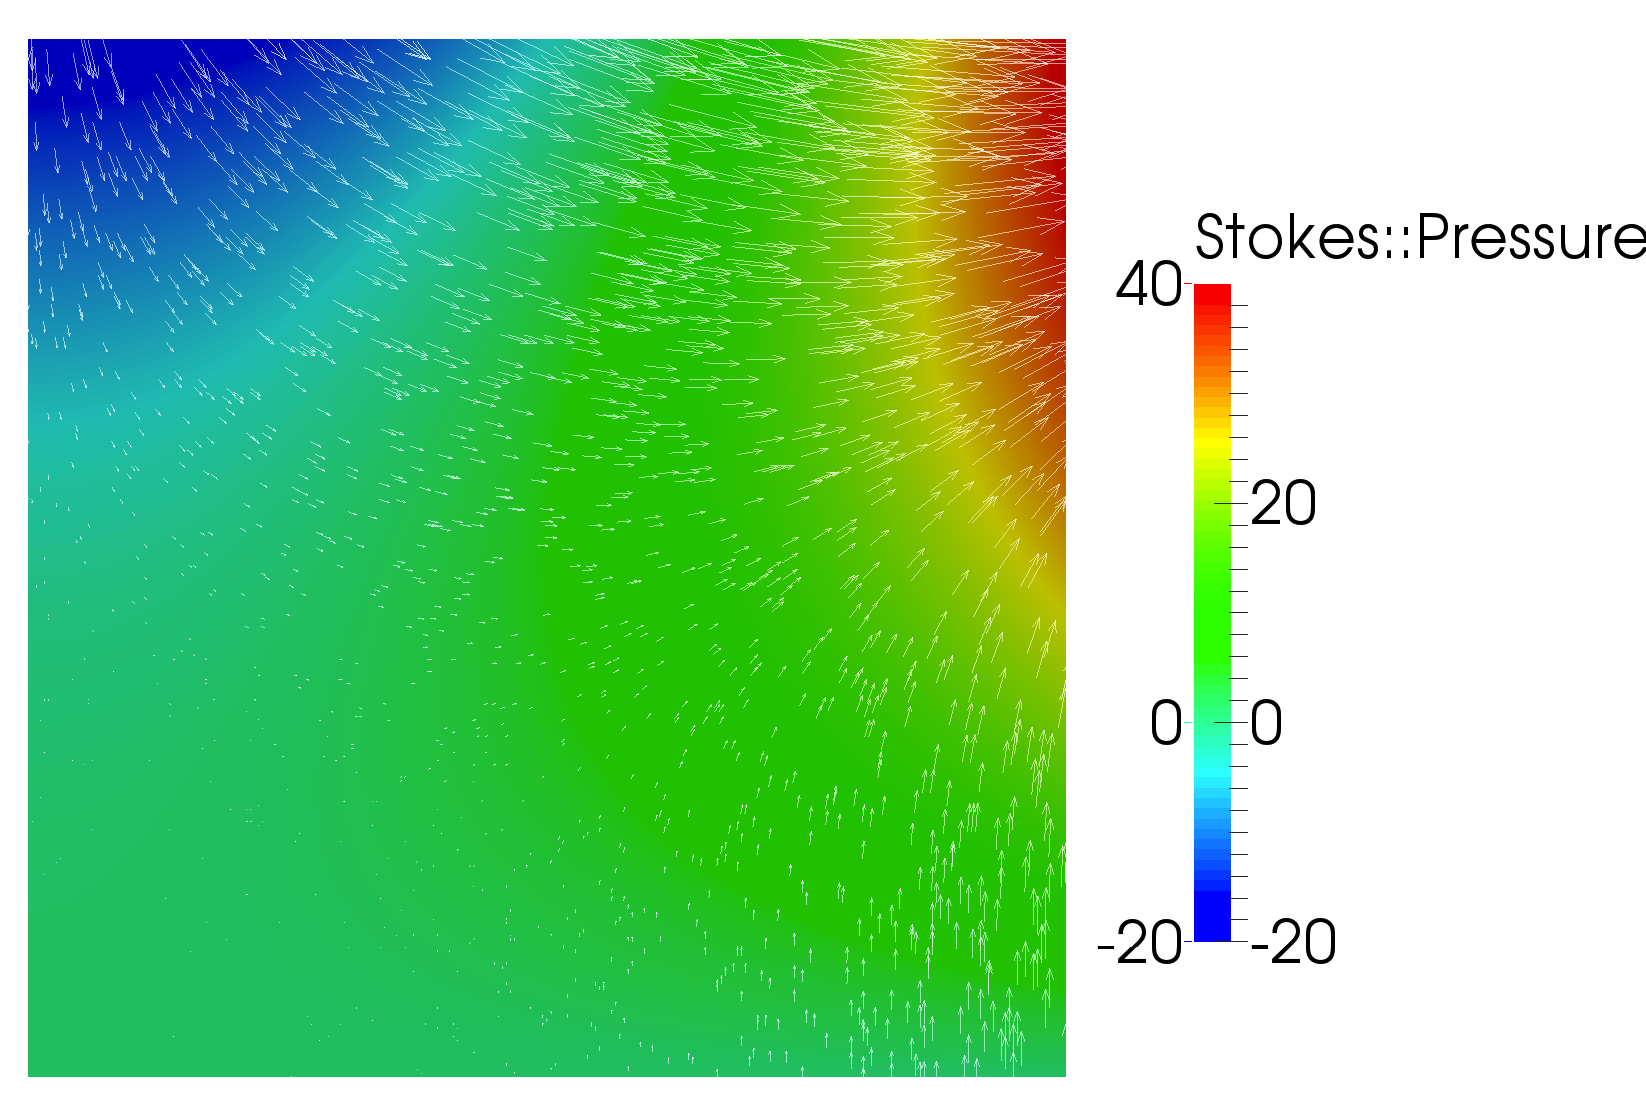
\includegraphics[width=.7\textwidth]{figures/stokes_flow.png}
  \caption{MMS solution of Stokes equation from
    \cite{elman_finite_2005} showing the pressure field in the background color map and the velocity field shown with arrows.}
  \label{fig:stokesMMS}
\end{figure}

\section{Solution using \TF}
\label{sec:solution-using-tf}

However, setting this problem up in \TF{} is not
much more difficult than solving the scalar Poisson equation.  The
principal changes from the mms problem \texttt{poisson.tfml} are
\begin{itemize}
\setlength{\itemsep}{0em}
\item We  change the domain from $[0,1]\times[0,1]$ to
  $[-1,1]\times[-1,1]$ (mesh changes to Rectangle)
\item The system now includes two fields for $\vec{v}$ and $p$
\item The field Velocity, is now vector valued and should be in
  $[P_{2}\times P_{2}]$
\item The field Pressure is a scalar in $P_{1}$ with no Boundary
  conditions and a constant null space.
\item Each of the fields will require diagnostics, IC's and BC's
\item The forcing term and boundary conditions just need to be made
  consistent for this MMS problem
\item The non-linear residual needs to change to the above UFL
\end{itemize}

A fully worked out \texttt{tfml} file for this problem using a direct
solver along with a testharness file \texttt{stokes.shml} for running
the convergence test can be
found in \texttt{\$TF\_HOME/share/terraferma/tutorials/stokes/isoviscous/mms/mms\_direct}.
The solution is shown in Figure \ref{fig:stokesMMS}.  Figure
\ref{fig:stokes_convergence}  shows the convergence behavior for both
velocity and pressure and shows larger errors for pressure which
decrease as $h^{2}$ compared to errors for velocity which scale as
$h^{3}$. This plot can be reproduced using

\pagebreak{}
\begin{lstlisting}[style=Bash]
$ cd $TF_HOME/share/terraferma/tutorials/stokes/isoviscous/mms/mms_direct
$ tfsimulationharness --test stokes.shml
\end{lstlisting} %$



\begin{figure}[htbp!]
  \centering
  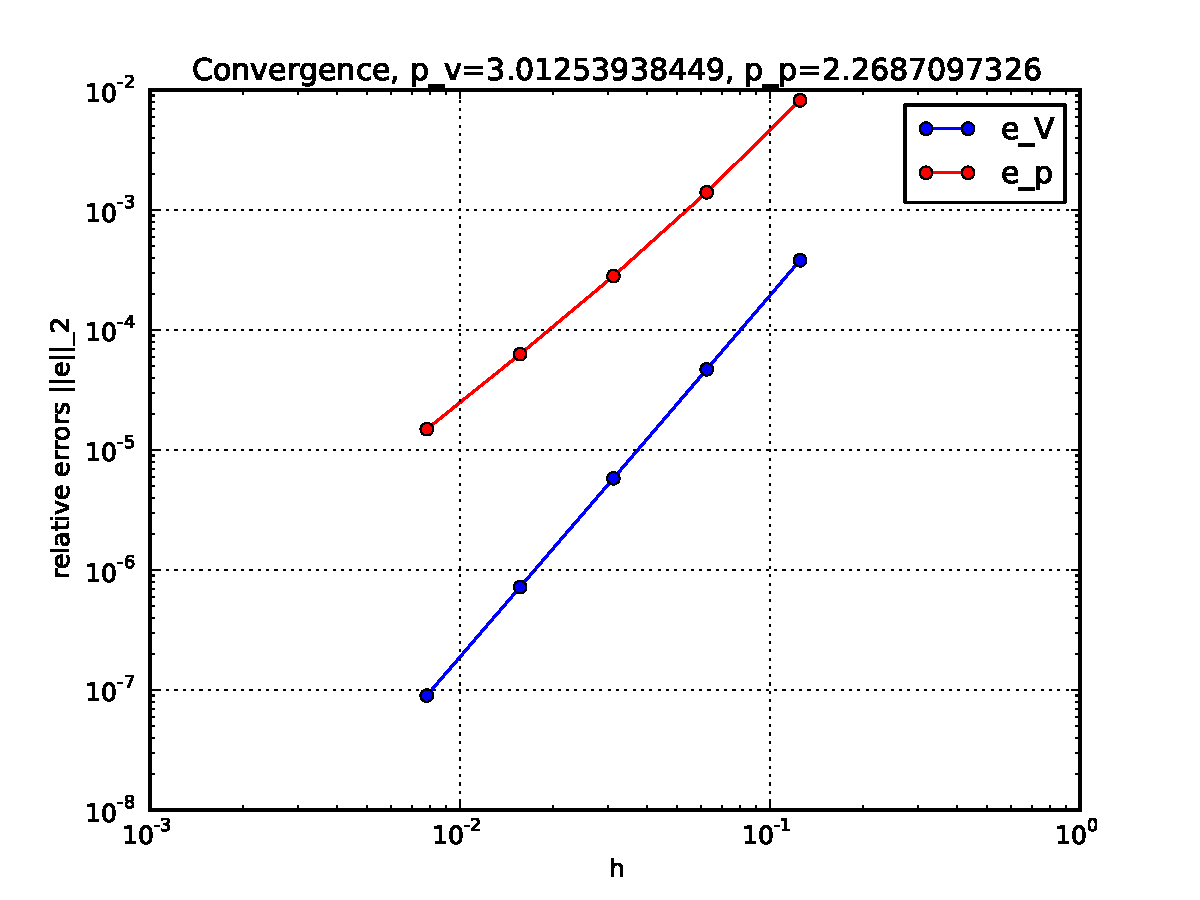
\includegraphics[width=.7\textwidth]{figures/Stokes_convergence.pdf}
  \caption{Convergence behavior of stokes solution for isoviscous
    stokes using P2-P1 ``Taylor-Hood'' mixed elements.}
  \label{fig:stokes_convergence}
\end{figure}

%\pagebreak{}

In more detail, the specific steps required to modify the poisson mms
problem to solve Stokes are as follows.
\begin{steps}{Step}
\item Make a new tfml file
  \begin{lstlisting}[style=Bash]
$ mkdir mystokes
$ cd mystokes
$ cp $TF_HOME/share/terraferma/tutorials/poisson/mms/poisson.tfml stokes.tfml
$ diamond stokes.tfml &
  \end{lstlisting}%$
\item \textbf{Change the geometry:} Under \texttt{geometry->Mesh},
  \begin{steps}{step}
  \item Change source from UnitSquare to Rectangle
  \item Set \texttt{lower\_left} to $-1.,-1.$
  \item Set \texttt{upper\_right} to $1.,1.$
  \item Set \texttt{number\_cells} to $32,32$
  \item Set \texttt{diagonal} to \texttt{right/left}
  \end{steps}
\item \textbf{Change io parameters}
  \begin{steps}{step}
  \item Change \texttt{output\_base\_name} to \texttt{stokes}
  \item Change \texttt{visualization->element} to (P2)
  \end{steps}
\item \textbf{Modify System Poisson to System Stokes}
  \begin{steps}{step}
  \item Change the system name to  Stokes (the \texttt{ufl\_symbol (global)}
    remains the same as \texttt{us})
  \item Change the field \texttt{u} to \texttt{Velocity}
    \begin{itemize}{}
    \item change the field name to \texttt{Velocity}
    \item change the \texttt{ufl\_symbol (global)} to \texttt{v}
    \end{itemize}
  \item Modify the velocity field to be vector valued [P2,P2]
    function.   Under \texttt{type (Function)}
    \begin{itemize}{}
    \item Change \texttt{rank} from Scalar to \texttt{Vector}
    \item Set \texttt{element} to P2
    \end{itemize}
  \item Set the velocity Initial Condition to constant $[0.,0.]$
  \item Set the Velocity Boundary conditions to the MMS solution
    \begin{itemize}
    \item Activate a new \texttt{boundary\_condition} under
      \texttt{rank} and name it \texttt{mms}
    \item Set \texttt{boundary\_ids} to \texttt{1 2 3 4} (all boundaries)
    \item Under \texttt{sub\_components (All)} choose \texttt{type (Dirichlet)
        -> python}
    \item Add a new python function to evaluate the velocity boundary
      conditions as a function of $x$ using Equation (\ref{eq:stokes-mms}).
      \begin{lstlisting}[style=Python]
def val(x):
  u = 20.*x[0]*x[1]**3
  v = 5.*(x[0]**4 - x[1]**4)
  return [u,v]
      \end{lstlisting}
    \end{itemize}
  \item \textbf{Check the diagnostics for a vector valued
      velocity}. Just check that only
    \texttt{include\_in\_visualization} and
    \texttt{include\_in\_statistics} are chosen (although feel free to try any
    other option as well)
    \item \textbf{add a new field for Pressure}
      \begin{itemize}
      \item Either create a new Field tab or copy the Velocity tab and
        rename to Pressure
      \item Set the \texttt{ufl\_symbol (global)} to \texttt{p}
      \item Choose \texttt{type (Function)} and
        \begin{itemize}
        \item Set \texttt{rank (Scalar)}
        \item Set \texttt{element (P1)}
        \item Set \texttt{initial\_condition} to a constant (0.0)
        \end{itemize}
      \item \textbf{Set a reference point:}  Stokes with all Dirichlet 
        BC's for velocity is actually singular allowing an arbitrary
        constant in the pressure.  There are multiple ways in TF to
        remove this singularity.  For direct solvers, we can set  a single reference
        point where the pressure is constrained to be zero. For
        the MMS solution given here, $p=0$ at coordinates $(0.,0.)$.
        To set this point.  Activate the \texttt{reference\_point
          (Point)} tab and set the coordinates to $(0.,0.)$.
      \end{itemize}
  \item \textbf{Set the diagnostics for Pressure}: add \texttt{include\_in\_visualization} and \texttt{include\_in\_statistics}
  \item \textbf{Set the rhs function f:} under \texttt{coefficient (f)}
    \begin{itemize}
    \item make sure the \texttt{ufl\_symbol} is set to \texttt{f}
    \item Set the type to \texttt{Constant}
    \item Set the rank to \texttt{Vector}
    \item Set \texttt{value (WholeMesh)->constant (dim)} to $[0.,0.]$
    \end{itemize}
  \item \textbf{remove the function g} (if you're modifying from
    mms/poisson.tfml there will be an extra coefficient \texttt{g},
    just remove this tab using the - button.
  \item \textbf{Set a coefficient for the analytic solution for Velocity}
    \begin{itemize}
    \item Modify (or add) a coefficient
      \texttt{AnalyticSolutionVelocity} and set its
      \texttt{ufl\_symbol} to \texttt{ve}
    \item Set its \texttt{type} to \texttt{Expression}
    \item \texttt{rank (Vector)}
    \item \texttt{Element (P2)}
    \item \texttt{value (WholeMesh)->python} with the python function
      \begin{lstlisting}[style=Python]
# exact solution for velocity
def val(x):
  u = 20.*x[0]*x[1]**3
  v = 5.*(x[0]**4 - x[1]**4)
  return [u,v]
      \end{lstlisting}
    \end{itemize}
 \item \textbf{Set a coefficient for the analytic solution for Pressure}
    \begin{itemize}
    \item Add (or copy) a coefficient
      \texttt{AnalyticSolutionPressure} and set its
      \texttt{ufl\_symbol} to \texttt{pe}
    \item Set its \texttt{type} to \texttt{Expression}
    \item \texttt{rank (Scalar)}
    \item \texttt{Element (P1)}
    \item \texttt{value (WholeMesh)->python} with the python function
      \begin{lstlisting}[style=Python]
# exact solution for Pressure
def val(x):
  p = 60.*x[0]**2*x[1] - 20*x[1]**3
  return p
      \end{lstlisting}
    \end{itemize}
  \item Change the residual from poisson to Stokes with
    \begin{lstlisting}[style=UFL]
# scaled viscosity term
eta = 1.

Fv = (inner(sym(grad(v_t)), 2.*eta*sym(grad(v_i))) 
       - div(v_t)*p_i   - inner(v_t,f_i))*dx
Fp = -p_t*div(v_i)*dx

F = Fv + Fp
    \end{lstlisting}
  \item\textbf{ Set some Functionals for calculating errors}
 \begin{itemize}
 \item rename the functional \texttt{uL2NormErrorSquared} to \texttt{VelocityL2NormErrorSquared} 
    \item and change  the functional to
      \begin{lstlisting}[style=Ufl]
        errv2 = inner((v-ve),(v-ve))*dx
      \end{lstlisting}
      and change its \texttt{ufl\_symbol} to \texttt{errv2}.
    \item Add another functional \texttt{VelocityL2NormSquared}
      \begin{lstlisting}[style=Ufl]
        l2v2 = inner(v,v)*dx
      \end{lstlisting}
      and set its \texttt{ufl\_symbol} to \texttt{l2v2}.
    \item repeat for the pressure functionals (diamond copy and paste can be
      quite useful here) to make two more functionals
      \begin{itemize}
      \item \texttt{PressureL2NormErrorSquared}
        \begin{lstlisting}[style=Ufl]
        errp2 = (p - pe)**2*dx
      \end{lstlisting}
    \item \texttt{PressureL2NormSquared}
        \begin{lstlisting}[style=Ufl]
        l2p2 = p**2*dx
      \end{lstlisting}
      \end{itemize}

    \end{itemize}


   \end{steps}
 \item \textbf{Remove the system Error} (unless you want to visualize
   the errors in which case you'll need to modify this system).
 \item \textbf{Test the build using either}
   \begin{lstlisting}[style=Bash]
$ tfbuild stokes.tfml
$ cd build
$ make -j 3
$ make run
$ cd ..
   \end{lstlisting}
   \textbf{or}
   \begin{lstlisting}[style=Bash]
$ cp $TF_HOME/share/terraferma/tutorials/stokes/isoviscous/mms/mms_direct/stokes.shml .
$  tfsimulationharness --build stokes.shml
\end{lstlisting} %$
 \item \textbf{Run the convergence tests:}
   \begin{lstlisting}[style=Bash]
$ cp $TF_HOME/share/terraferma/tutorials/stokes/isoviscous/mms/mms_direct/stokes.shml .
$  tfsimulationharness --test stokes.shml
\end{lstlisting} %$
(Note: you might need to modify some of the names in the
\texttt{.shml} file and you should also make sure you have enough
memory to run large ($\geq 128\times128$ cell) direct solves. 
\end{steps}


%\pagebreak{}
\section{Themes and Variations}
\label{sec:themes-variations}

Many of the simple variations demonstrated in Chapter
\ref{cha:poiss-equat-unit} for Poisson's Equation are readily adapted
to the Stokes problem.  For example Figure \ref{fig:stokes_gmsh} shows
an isoviscous Stokes flow solution on a more complicated mesh
generated by gmsh.  A fully worked out example 
can be found in
\texttt{\$TF\_HOME/share/terraferma/tutorials/stokes/isoviscous/gmsh}.
In particular this example includes  a test-harness file
\texttt{stokes.shml} that demonstrates how to use the test harness to
call gmsh to generate the mesh that the model depends on.  The full
problem including the meshes can be built and run using
\begin{lstlisting}[style=Bash]
$ tfsimulationharness --test stokes.shml
\end{lstlisting} %$



\begin{figure}[htbp!]
  \centering
  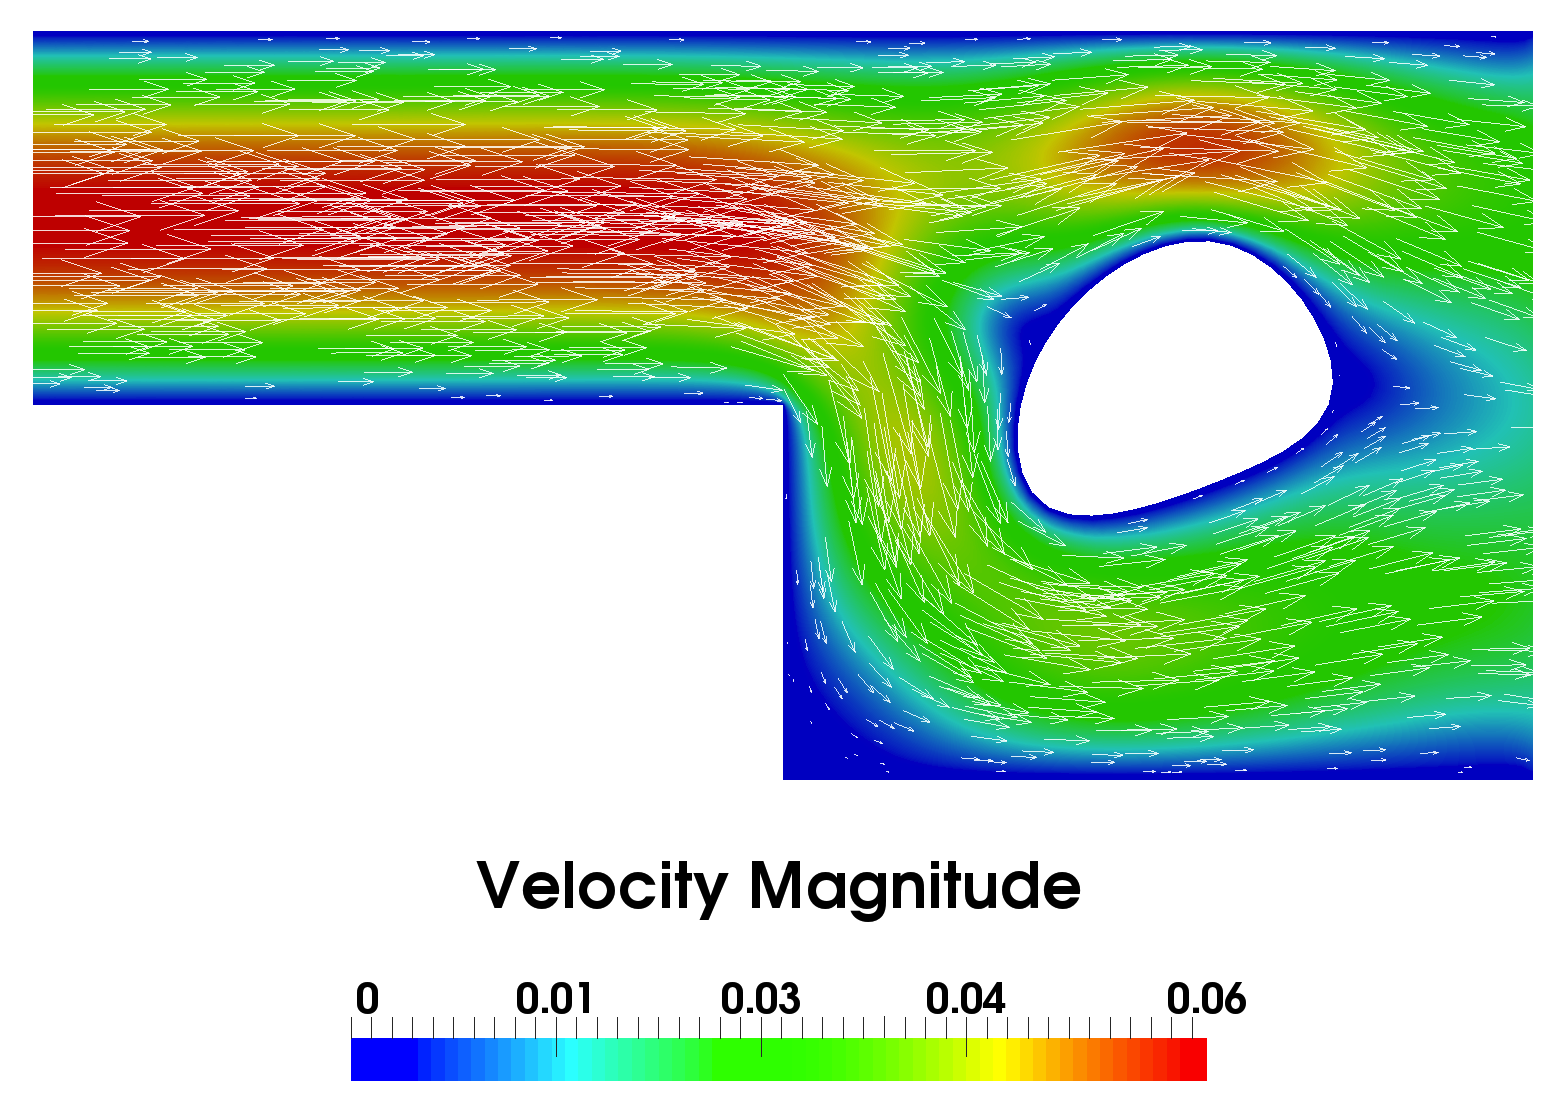
\includegraphics[width=0.7\textwidth]{figures/stokes_gmsh.png}
  \caption{\small Isoviscous Stokes solution for a more complex geometry.
    Boundary conditions are parabolic inflow $u(0,y)=(y-1/2)(1-y),
    v=0$ on the left-hand boundary, Natural outflow boundary
    conditions on the right ($x=2$), and no-flow $\vec{v}=\vec{0}$ on
    all other boundaries including the interior hole.  This example
    uses boundary id's generated by gmsh.}
  \label{fig:stokes_gmsh}
\end{figure}

\subsection{Iterative Solvers and Fieldsplit preconditioners}
\label{sec:iterative-solvers-1}

For moderate sized problems in 2-D, sparse-direct solvers can be
efficient and extremely robust methods.  However, for larger problems
and particularly in 3-D we need to move to iterative solvers.  There
is a large literature on iterative solvers for Stokes equation, 
%% FIXME and future versions of this tutorial will hopefully address
%% at least some of this. 
however, here we will just present one solver for isoviscous
Stokes presented in \cite{elman_finite_2005} as a means of introducing
PETSc's fieldsplit block-preconditioners as implemented in \TF{}.

The discrete inner linear solve in a Newton iteration for Stokes can
be written
\begin{equation}
  \label{eq:21}
     \left[
\begin{array}{cc}
  K & G  \\
  G^{T} & 0 \\
  \end{array}
  \right]
  \left[
    \begin{array}{c}
      \delta \vec{v} \\
      \delta p \\
    \end{array}
  \right] = -\left[
    \begin{array}{c}
      F_{\vec{v}} \\
      F_{p}\\
    \end{array}
  \right]
\end{equation}

May and Moresi \cite{may_preconditioned_2008} present a large number of block
preconditioning schemes for this problem including Schur Complement
Reduction based schemes (SCR) and Fully coupled block preconditioners
(FC).  Here we will discuss one FC upper triangular block
preconditioner
\begin{equation}
  \label{eq:ch3-22}
    \mat{J}_{\text{PC}} =   \left[
\begin{array}{cc}
  K & G  \\
  0 & \hat{S} \\
  \end{array}
  \right]
\end{equation}
where
\begin{displaymath}
  \hat{S} = \int \frac{1}{\eta} p_{t}p dx
\end{displaymath}
is the viscosity weighted pressure mass matrix which has been shown to
be a useful approximation to the Schur Complement $S$ for variable
viscosity problems\cite{grinevich_iterative_2009,ur_rehman_iterative_2011}.  The solution
strategy is to right-precondition the full solution $u=(\vec{v},p)$
with $J_{\text{PC}}$ using a fieldsplit block preconditioner that
first applies an approximate solve to
\begin{equation}
  \hat{S}\delta p = -F_{p}
\label{eq:ch3-23}
\end{equation}
using a lightweight SOR preconditioned CG iterative solver on
$\hat{S}$, then solves
\begin{equation}
  K\delta\vec{v} = -F_{v} - G\delta p
\label{eq:ch3-24}
\end{equation}
using an approximate iterative solve for the viscosity block $K$. In
particular, here we use a second fieldsplit preconditioned iterative
solver for the $K$ block where we use 1 FGMRES iteration on the full
$K$ block, preconditioned by one V-cycle of  an algebraic multi-grid
solver (hypre) on each of the diagonal blocks of $K$. This is
effectively the same pre-conditioner solver used in the RHEA code
\cite{burstedde_large-scale_2013}. Schematically, the tree structure of the nested solver/pre-conditioner set up is shown in
Figure \ref{fig:fieldsplit_stokes}
\begin{figure}[h!]
  \centering 
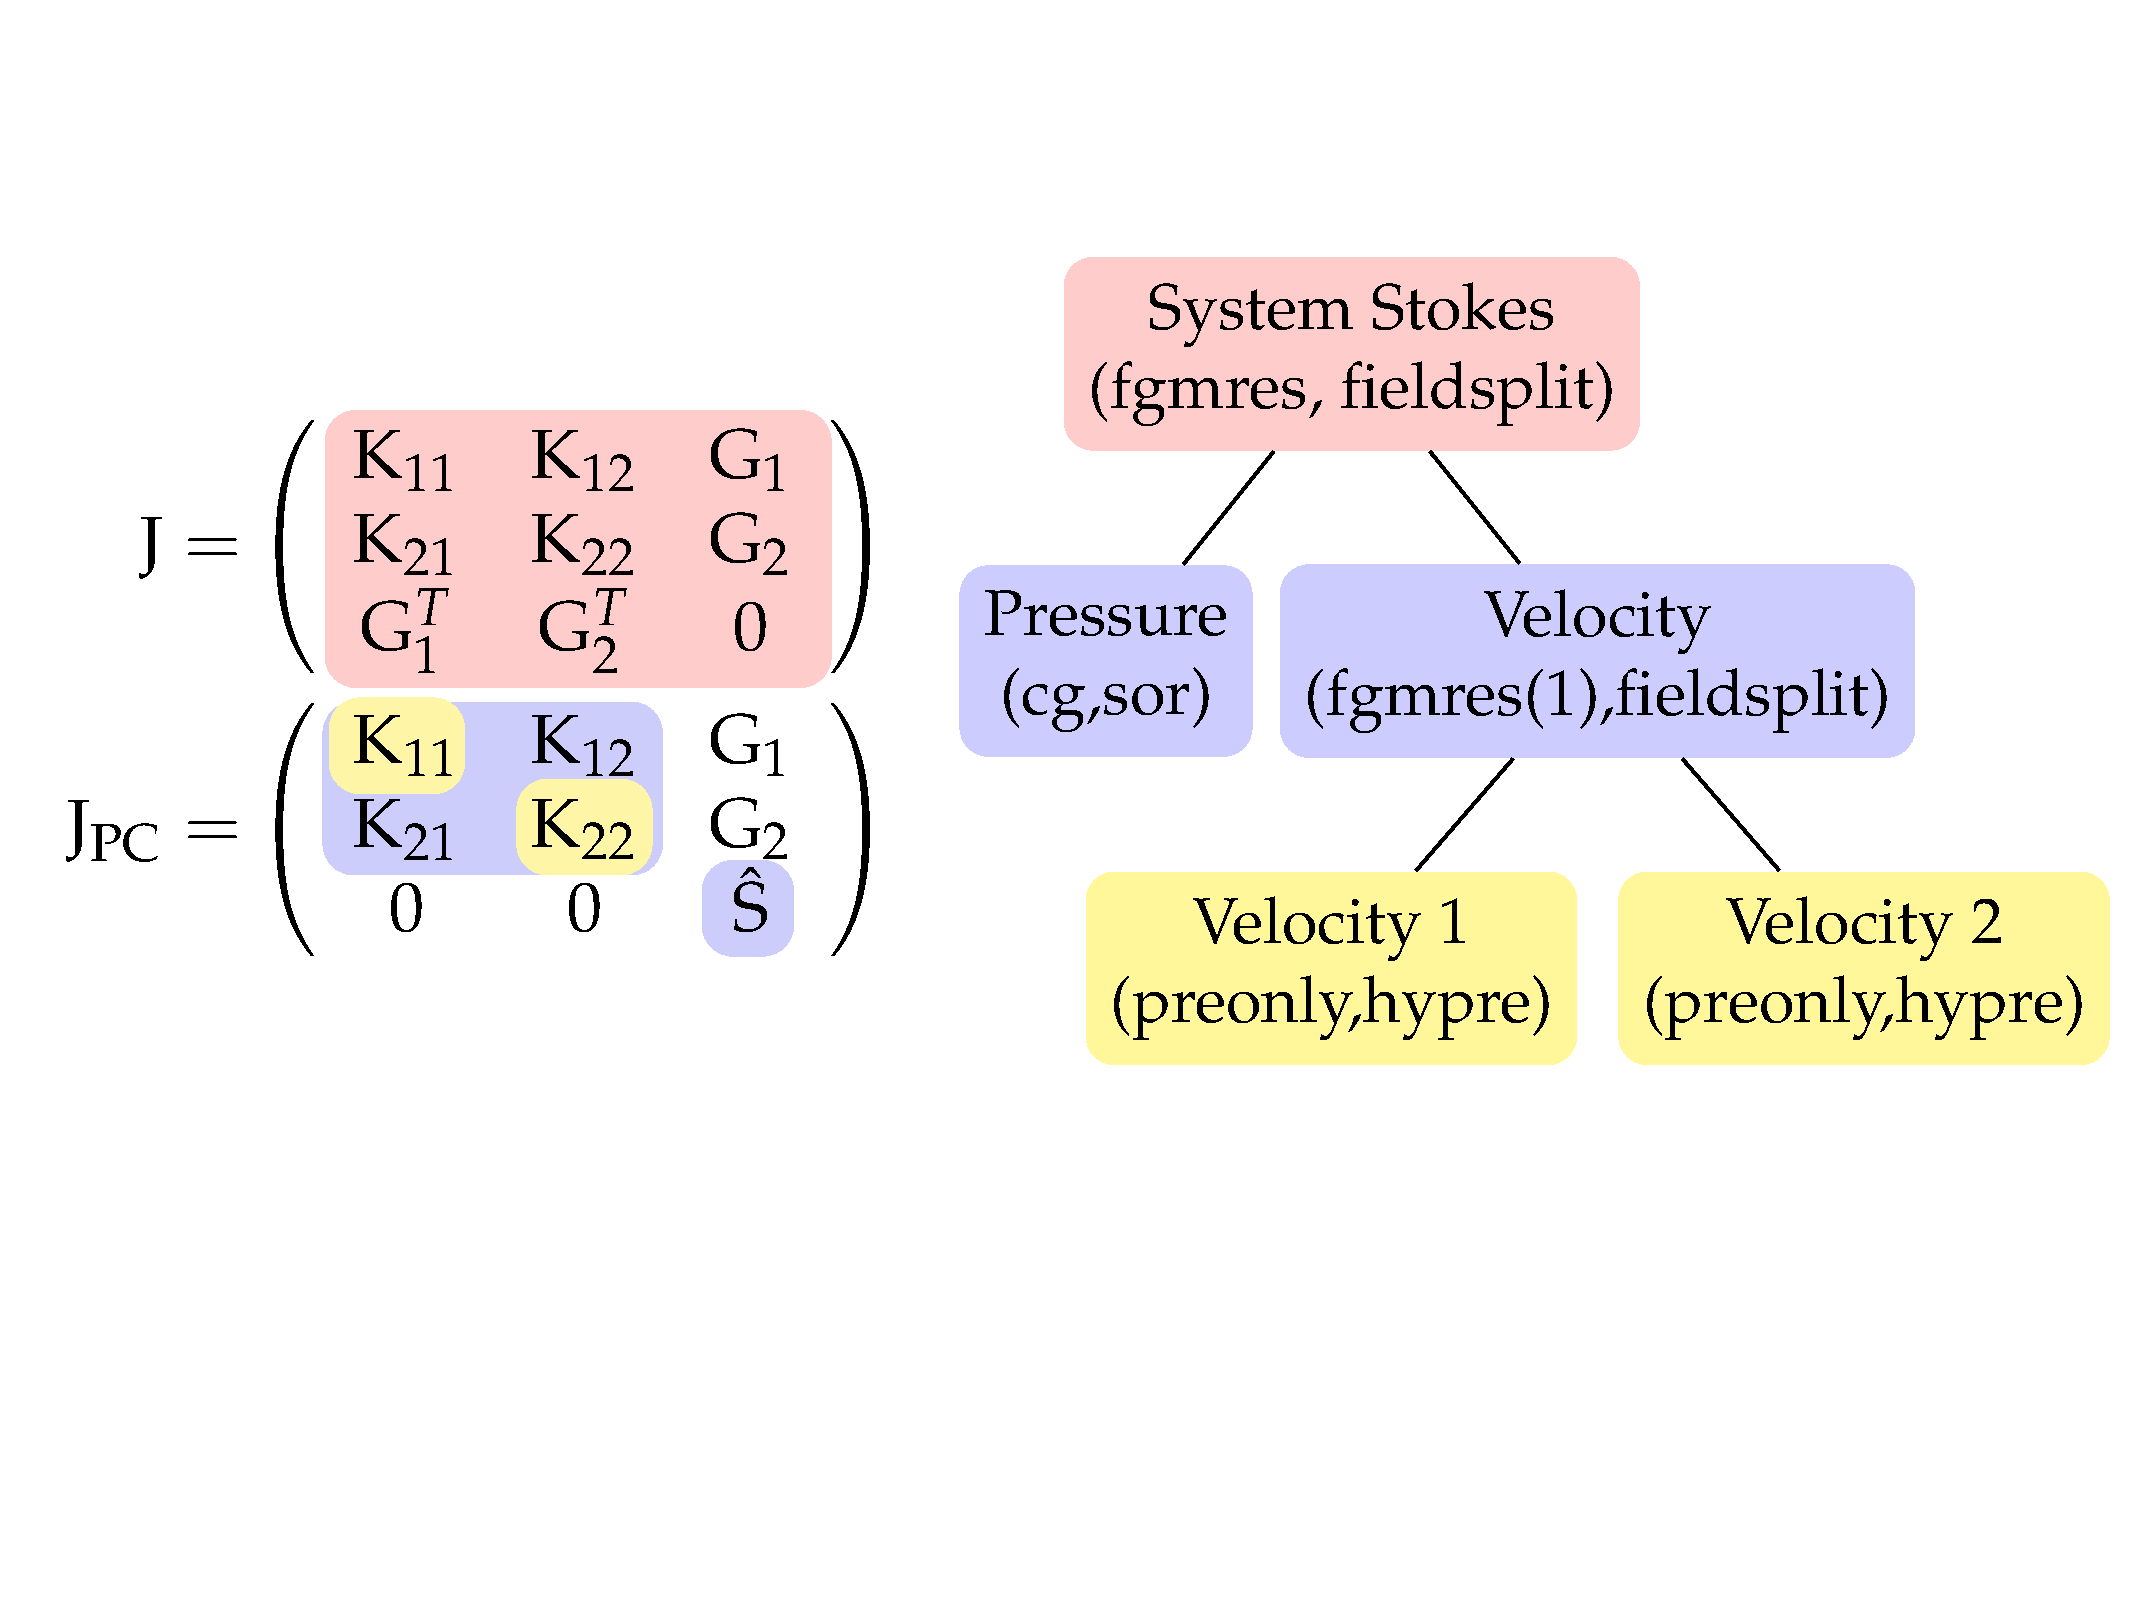
\includegraphics[width=.8\textwidth]{figures/Stokes_block_preconditioners.pdf}
%% way to fragile TikZ stuff here...but useful for making the pdf I
%% eventually used
% \begin{minipage}{0.45\textwidth}
% %\vspace*{-3cm}
% \begin{center}
% \begin{align*}
% \mat{J} =& \left(\begin{array}{ccc}
% \tikzmark{K11}{$\mat{K}_{11}$} & \mat{K}_{12} & \mat{G}_1 \\
% \mat{K}_{21} & \mat{K}_{22} & \mat{G}_2  \\
% \mat{G}_1^T    & \mat{G}_2^T    &  \tikzmark{saddle}{$\mat{0}$}     \\
% \end{array}\right) \\
% \mat{J}_{\text{PC}} = & \left(\begin{array}{ccc}
% \tikzmark{K11PC}{$\mat{K}_{11}$} & \mat{K}_{12} & \mat{G}_1   \\
% \mat{K}_{21} & \tikzmark{K22PC}{$\mat{K}_{22}$} & \mat{G}_2   \\
% \mat{0}    & \mat{0}    & \tikzmark{saddlePC}{$\mat{\hat{S}}$}  \\
% \end{array}\right) \\
% \end{align*}
% \end{center}
% %\vspace*{1cm}
% \end{minipage}
% \hspace{1cm}
% \begin{tikzpicture}[shape=rectangle, rounded corners, align=center,
%     level distance=1.5cm,
%     level 1/.style={sibling distance=2.4cm},
%     level 2/.style={sibling distance=2.6cm}]
%    % level 3/.style={sibling distance=2cm}]
%     % \node [hide on=1, fill=green!20, align=center, font=\footnotesize] {System\\(fgmres, fieldsplit)} [edge from parent fork down]
%     % child [hide on=1] {node [fill=red!20, align=center, font=\footnotesize] {Temperature\\(gmres, ilu)}}
%     \node [fill=red!20, align=center, font=\small] {System Stokes\\(fgmres, fieldsplit)}
%       child  {node [fill=blue!20, align=center, font=\small] {Pressure\\(cg,sor)}}
%       child {node [fill=blue!20, align=center, font=\small] {Velocity\\(fgmres(1),fieldsplit)}
%         child {node [fill=yellow!50, align=center, font=\small] {Velocity 1\\(preonly,hypre)}}
%         child 
%         {node [fill=yellow!50, align=center, font=\small]
%           {Velocity 2\\(preonly,hypre)}}
% };
% \end{tikzpicture}
  \caption{\label{fig:fieldsplit_stokes} Overview of the tree
    structure of nested fieldsplit preconditioners used  for an
    iterative solver for Stokes equation.  $J$ is the expanded
    Jacobian for a 2-dimensional Stokes problem with two-components of
  velocity and pressure.  $J_{\text{PC}}$ is the approximate Jacobian
  used as a pre-conditioner.  At the highest level, we solve $J\delta
  u=-F$ using a pre-conditioned FGMRES scheme (red).  This is
  right pre-conditioned by first solving $J_{\text{PC}}\delta u = -F$
  using $\sim5$ iterations  of (CG,SOR) on the pressure mass matrix
  $\hat{S}$ followed by one iteration of FGMRES on the full $K$ block
  (blue).  The $K$ block is further  preconditioned by a diagonal
  block-preconditioner with one V-cycle of   algebraic multi-grid on
  the diagonal blocks of $K_{11}, K_{22}$ (yellow).}
 \end{figure}

Given the natural tree structure of xml and Spud.  This
nested-fieldsplit preconditioner is relatively straightforward to
describe in \TF{}.  Step-by-Step instructions for modifying the Stokes
MMS problem with a direct solver are as follows (and a fully worked
out example can be found in
\texttt{\$TF\_HOME/share/terraferma/tutorials/stokes/isoviscous/mms/mms\_iterative}.

\begin{steps}{Step}
\item Make a new tfml file from one with a direct solver
  \begin{lstlisting}[style=Bash]
$ mkdir mymms_iterative
$ cd mymms_iterative
$ cp $TF_HOME/share/terraferma/tutorials/stokes/isoviscous/mms/mms_direct/stokes.tfml .
$ diamond stokes.tfml &
  \end{lstlisting}%$
\item \textbf{Remove the reference point in Pressure:} This stokes
  problem is still singular, but we will address it by projecting out
  the null space in the iterative solvers.  So we need to deactivate the
  reference point control tab
  \begin{lstlisting}[style=Python]
    system (Stokes)
       field (Pressure)
         type (Function)
           rank (Scalar)
             reference_point (Point)
  \end{lstlisting}
\item \textbf{Add an additional form for the preconditioner for the
    Jacobian} To implement the upper triangular preconditioner in Eq.\
  (\ref{eq:ch3-22}) we need to add one more form for the preconditioner
  (PETSc, allows passing a separate preconditioning matrix to KSP or
  SNES). Do the following
  \begin{steps}{step}
  \item Under \texttt{nonlinear\_solver
    (Solver)}$\rightarrow$\texttt{type (SNES)} activate the optional
  tab \texttt{form (JacobianPC)} and set the form to the ufl code
  \begin{lstlisting}[style=UFL]
Jpcv = (inner(sym(grad(v_t)), 2.*eta*sym(grad(v_a))) - div(v_t)*p_a)*dx
Jpcp = -p_t*p_a/eta*dx

Jpc = Jpcv + Jpcp
  \end{lstlisting}
Alternatively,  we could be lazy and just recalculate the entire
Jacobian and add the  block $\hat{S}$ using
\begin{lstlisting}[style=UFL]
Jpc = derivative(F,us_i,us_a) - p_t*p_a/eta*dx
\end{lstlisting}
although this will also assemble the $G^{T}$ block.
\item Set the \texttt{ufl\_symbol} to
  \texttt{Jpc}.
\item You might also want to activate and set the
  \texttt{quadrature\_degree} to 3 to keep all the Jacobians and
  residuals to the same order of quadrature.
  \end{steps}

\item \textbf{Change the linear solver}.  Now we need to replace the
  direct solver \texttt{(preonly,LU)} with the nested
  fieldsplit-preconditioned fgmres \texttt{(fgmres,fieldsplit)}
  discussed above.  Do the following
  \begin{steps}{step}
  \item Change the iterative solver to \texttt{fgmres} and set the
    following convergence settings:
    \begin{itemize}
    \item restart = 30
    \item relative\_error = 1.e-15
    \item absolute\_error = 1.e-7 (you'll need to activate this but
      this combination of relative and absolute error, makes sure that
      the norm of the residual is reduced to the absolute error, which
      should be somewhat smaller than the truncation error of the MMS
      solution for accuracy.)
    \item max\_iterations = 50
    \item You might also want to turn on \texttt{monitors} for the
      \texttt{preconditioned\_residual}. These will be recorded in the
      log file.  You can also turn on \texttt{convergence\_file} to
      monitor detailed convergence behavior of the solver, but this
      will impact performance.
    \end{itemize}
  \item Change the preconditioner to \texttt{fieldsplit} and do the following
    \begin{enumerate}
    \item \textbf{Set the first fieldsplit (Pressure)}:
      \begin{itemize}
      \item name the first required fieldsplit Pressure
      \item Add a field named Pressure (this name should match that
        given in the system)
      \item Set the linear solver to iterative method (cg) with
        \texttt{relative\_error} 1.e-5 and \texttt{max\_iterations} = 50.
      \item Set the preconditioner to \texttt{(sor)}
      \end{itemize}
    \item \textbf{Set the second fieldsplit (Velocity)}:
      \begin{itemize}
      \item Add a second fieldsplit (named Velocity)
      \item add the field \texttt{Velocity}
        \item Set the linear solver to \texttt{fgmres} with
          \texttt{restart} 30, \texttt{relative\_error} 1.e-3,
          \texttt{max\_iterations} 1
        \item Set the preconditioner to \texttt{fieldsplit}
      \end{itemize}
    \item \textbf{Set additional Fieldsplits for the $K$ block} Here
      we will just use a single hypre algebraic multi-grid cycle on
      each of the diagonal blocks $K_{11}$ and $K_{22}$ in Figure \ref{fig:fieldsplit_stokes}.
      \begin{itemize}
      \item Under this second \texttt{preconditioner (fieldsplit)},
        set the \texttt{composite\_type} to \texttt{(additive)}.  This
        will only do a block-jacobi iteration on the diagonal blocks.\footnote{
        \texttt{composite\_type (multiplicative)} is block
        Gauss-Seidel and acts as either an upper or lower triangular
        block preconditioner depending on the order of the fields in
        the Jacobian and of the splits. \texttt{composite\_type
          (additive)} is a block-diagonal preconditioner.}
      \item Name the first fieldsplit Velocityx.
      \item Set the field name to \texttt{Velocity}
      \item add the \texttt{components} tab and set the component to 0
        (horizontal velocity)
      \item Set the \texttt{linear\_solver} for this fieldsplit to
        \texttt{(preonly,hypre)}
      \item Add a second fieldsplit for \texttt{Velocityy} (or use the
        copy/paste function in diamond to copy \texttt{Velocityx}.
      \item Repeat the above procedure but set \texttt{components} to 1.
      \end{itemize}
    \end{enumerate}
  \item \texttt{Remove the pressure Null space in the solver}: Under
    the top level \texttt{linear\_solver}, \texttt{(fgmres,fieldsplit)}, we need
    to remove the null-space associated with a constant pressure mode.
    \begin{enumerate}
    \item Activate the \texttt{remove\_null\_space} tab under the
      top-level \texttt{linear\_solver}.
    \item Name the \texttt{null\_space} \texttt{ConstantPressure}
    \item Under \texttt{null\_space} activate the field and name it \texttt{Pressure}
    \item Make sure the null space is set to \texttt{constant} (for
      more complicated spaces you can also provide a python routine to
      calculate the null-space)
    \end{enumerate}
  \end{steps}
\item \texttt{Make and run the program}
  \begin{lstlisting}[style=bash]
$ tfbuild stokes.tfml
$ cd build
$ make -j 2 
$ make run
\end{lstlisting}


\end{steps}

That should do it.  

\subsubsection{Replacing python expressions with C++ expressions}

While convenient, using python to evaluate expressions can be
expensive for large problems and also has the issue that python does
not share a name-space with dolfin and ufl and cannot always share or
use other derived functions.  For this reason, we also allow you to
directly overload the C++ Expressions from dolfin.  A full description
of the process is beyond the current scope of these tutorials, but
simplified examples are given in all the \texttt{.tfml} files in the
subdirectory \texttt{compare\_solvers}. Changing from
python to C++ expressions improves the overall run-time if python is
heavily used in the diagnostics (e.g. an estimate of the L2 norm of
the error against the manufactured solution) but has only minimal
impact on the solver and assembly time if python is only involved in
setting boundary conditions.

\subsubsection{Solver comparison}
\label{sec:solver-comparison}

Figure \ref{fig:stokes_solver_convergence_timing}  shows convergence
and timing results for three different stokes solvers available under
\texttt{\$TF\_HOME/share/terraferma/tutorials/stokes/isoviscous/mms/compare\_solvers}.
\begin{itemize}
\item \texttt{mms\_direct} uses a sparse-direct solver on the full Jacobian
\item \texttt{mms\_iterative} uses the nested fieldsplit iterative
  scheme described above
\item \texttt{mms\_fs\_direct} uses the same upper-triangular block
  preconditioner but uses a sparse direct solver on each of the
  $\hat{S}$ and $K$ blocks.
\end{itemize}
These plots can be reproduced by running
\begin{lstlisting}[style=Bash]
   $ cd $TF_HOME/share/terraferma/tutorials/stokes/isoviscous/mms/compare_solvers
   $ . ./environment
   $ tfsimulationharness --test compare_solvers.py 
 \end{lstlisting} %$
 (see the \texttt{README} file for more details).
These examples only show a few of the possible configurations of
solvers and preconditioners possible for Stokes under
TF. Nevertheless,  they demonstrate that optimal solvers can be
readily constructed and tested in TF.  


\begin{figure}[htbp!]
  \centering
 \textbf{a} 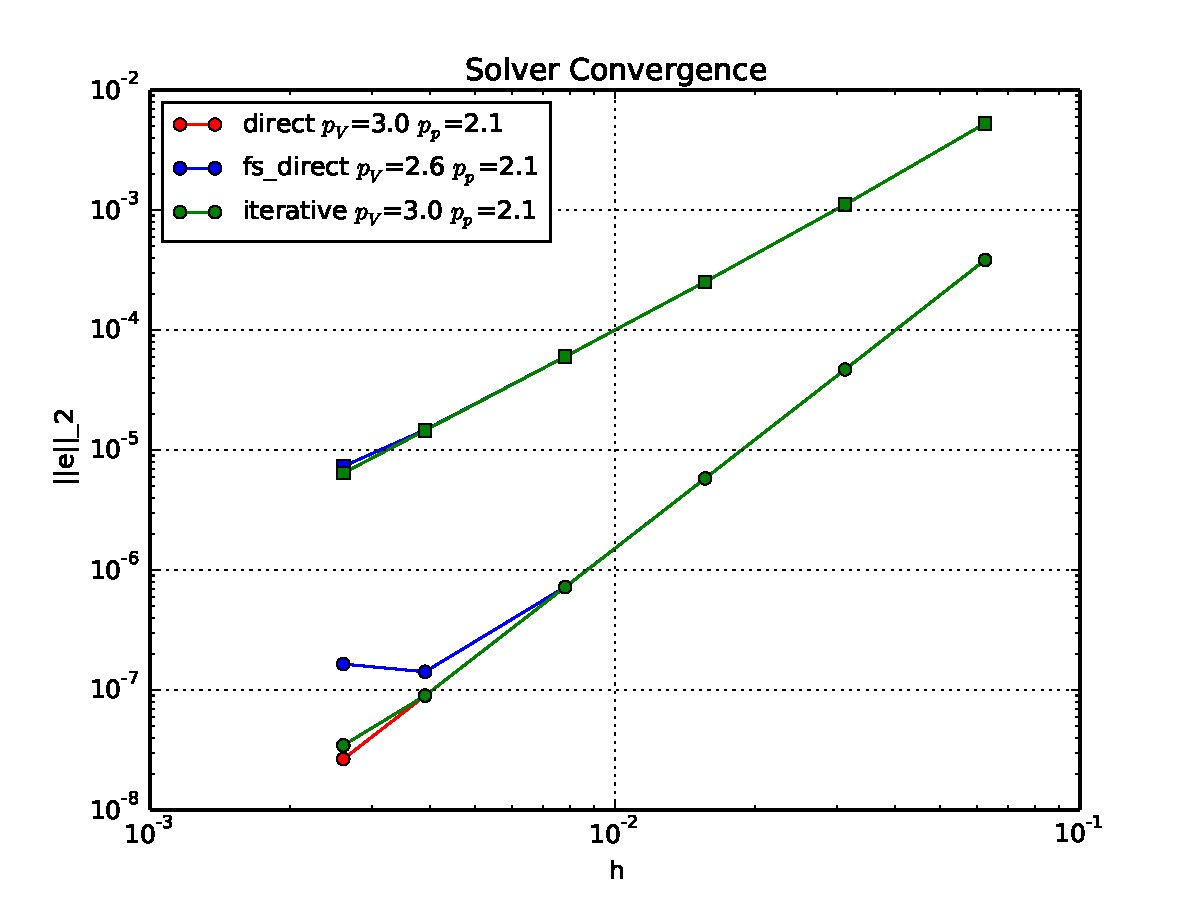
\includegraphics[width=.65\textwidth]{figures/Solver_comparison_convergence.pdf}\\
\textbf{b}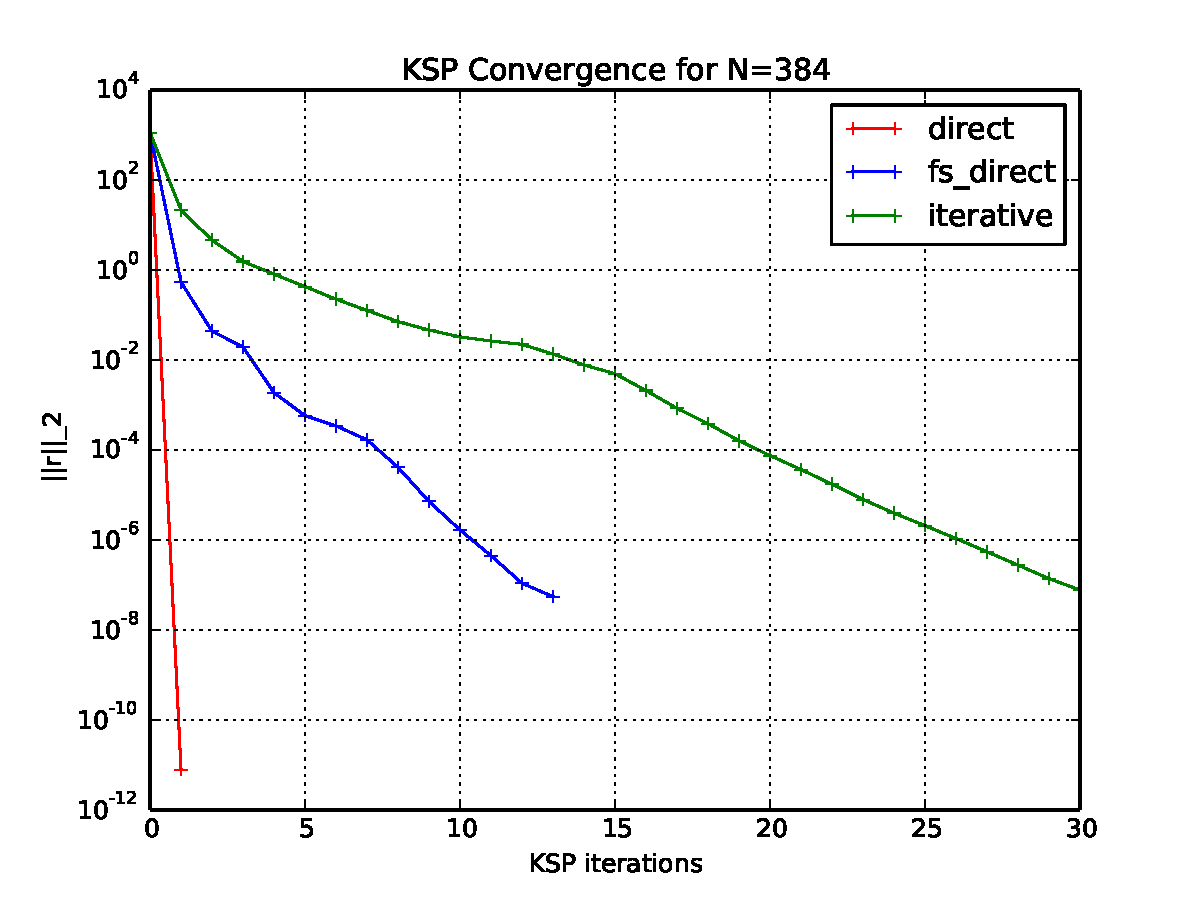
\includegraphics[width=.65\textwidth]{figures/Solver_Comparison_ksp_convergence.pdf}\\
\textbf{c}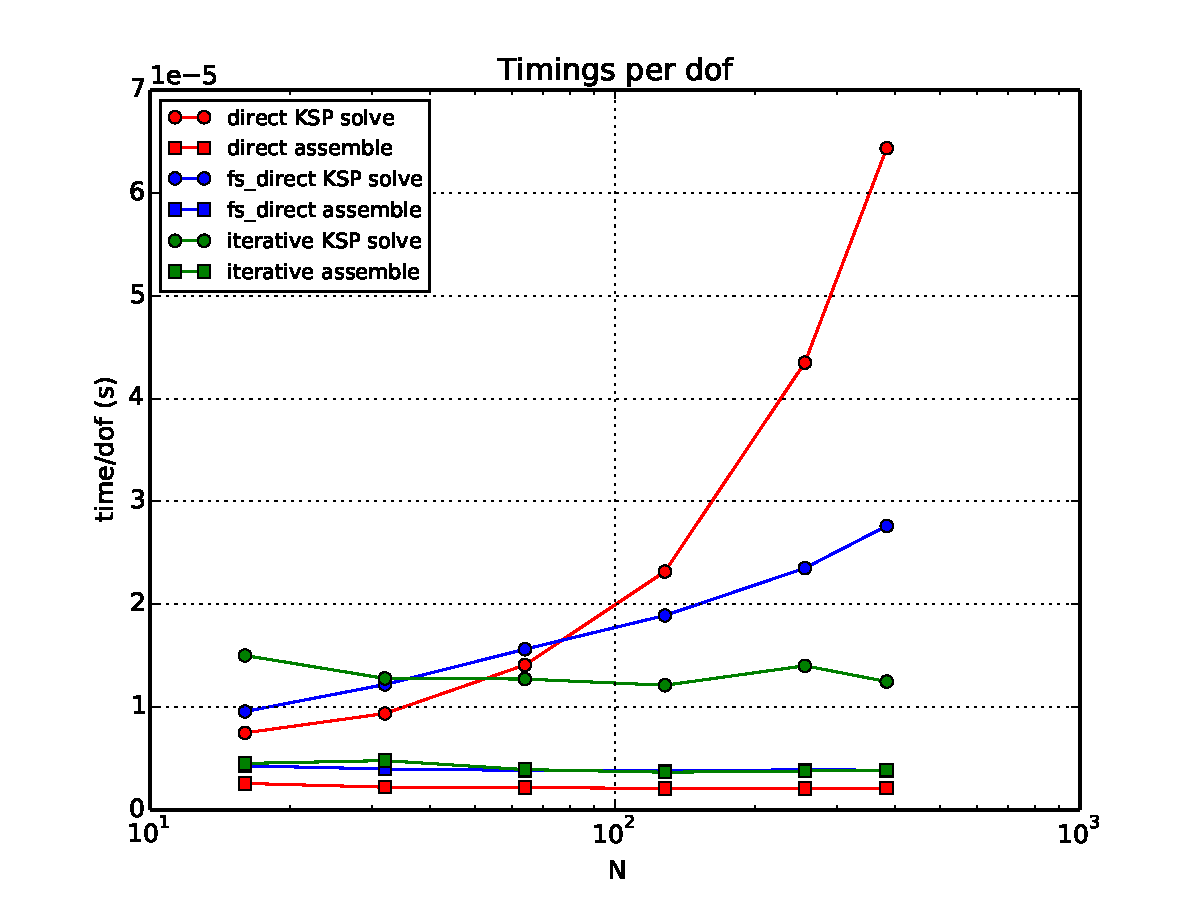
\includegraphics[width=.65\textwidth]{figures/Solver_Comparison_normalized_solver_timing.pdf}\\
  \caption{Comparison of Convergence and performance of MMS solution
    for three different solvers.  (\textbf{a}) relative error of
    solutions with respect to exact solution. (\textbf{b}) convergence behavior
    of the different linear solvers with respect to  the non-linear
    residual. (\textbf{c}) Performance.  Assembly and solver-time per
    degree of freedom.  Note increased assembly time for fieldsplit
    preconditioners reflects assembly of a second jacobian.
    \texttt{mms\_iterative} is optimal in that the timing scales only
    with $N$.}
  \label{fig:stokes_solver_convergence_timing}
\end{figure}

%%% Local Variables: 
%%% mode: latex
%%% TeX-master: "tftutorials"
%%% End: 

\chapter{Infinite Prandtl number Thermal Convection}
\label{cha:thermal-convection}

\section{Problem Overview}
\label{sec:convection_problem-formulation}

A model multi-physics  problem in Solid Earth Sciences is the solution of
infinite Prandtl number thermal convection, which couples Stokes
Equation (Chapter \ref{cha:stokes-equation}) for flow of a highly
viscous fluid to an advection-diffusion
equation for evolution of temperature, i.e.
\begin{align}
-\div\eta(\grad\vec{v} + \grad\vec{v}^{T}) + \grad p & = T\vec{k} \label{eq:rbconvv}\\ 
\div \vec{v} &= 0  \label{eq:rbconvp}\\
  \ppt{T} + \vec{v}\cdot\grad T - \frac{1}{\Ra}\nabla^2 T &= 0 \label{eq:rbconvT}
\end{align}
$\vec{v}$, $p$ are the dimensionless velocity and pressure, $T$ is
dimensionless temperature, and $\eta$ is dimensionless viscosity which
can be constant ($\eta=1$) or a function of $T$, $\vec{v}$ and/or $p$.
\begin{displaymath}
  \Ra = \frac{\rho g \alpha \Delta T h^{3}}{\eta_{0}\kappa}
\end{displaymath}
is the Rayleigh number for a layer of depth $h$, temperature
difference $\Delta T$ and reference viscosity $\eta_{0}$. 
% Do we need this next bit? 
% PvK: yes, useful since most geodynamicists use the other scaling.
Note, \eqref{eq:rbconvv}--\eqref{eq:rbconvT} scale velocity by
$\vec{v}=v_0\vec{v}'$ with
\begin{equation}
  \label{eq:4.6}
  v_0 = \frac{\rho g\alpha\Delta T h^{2}}{\eta_0}
\end{equation}
which is roughly the Stokes rise velocity of a buoyant blob of size $h$, rather than the
more standard ``diffusion velocity'' $v_0=\kappa/h$. This
scaling puts $1/\Ra$ in the diffusion term in \eqref{eq:rbconvT}, rather
than multiplying $T$ in \eqref{eq:rbconvv}. For large $\Ra$, \eqref{eq:rbconvT}
is dominantly advective with narrow diffusive boundary layers. 

Thermal convection is a good example of a multi-physics 
problem as it describes the coupled interactions of three fields;
velocity, pressure and temperature. Equations
\eqref{eq:rbconvv}--\eqref{eq:rbconvp} are  Stokes equations for incompressible viscous flow and are linear in $\vec{v}$ and $p$ if $T$ is
known and $\eta$ is independent of velocity.  Likewise,
\eqref{eq:rbconvT} is an advection-diffusion equation for $T$ and
appears linear in $T$ if $\vec{v}$ is known.   When all three fields are unknown then the coupled system $\vec{u}=\left(\vec{v}, p,
T\right)$ is non-linear because the velocity is a function of temperature and vice versa.  Adding additional coupling through more
complex rheologies, $\eta\left(T,\vec{v},p\right)$, only increases the
non-linearity of the system. These problems can be solved using either
Newton's method (N) or a Picard splitting scheme (P), both of which can
be implemented in \TF{}.


\subsection{Variational forms}

For this tutorial, we will reuse the setup for  Stokes using
``Taylor-Hood'' elements from 
Chapter \ref{cha:stokes-equation} and add to it an energy equation for
Temperature using quadratic $P_{2}$ elements. To solve the energy
equation, we start by discretizing the time derivative
using finite differences as
\begin{displaymath}
  \ppt{T}\approx(T_{i} - T_{n})/\Delta t
\end{displaymath}
where $T_{i}$ is our current estimate of the value of temperature at the new
time and $T_{n}$ is temperature at the previous time. We use a
$\theta$ scheme  for time-integration of the advection-diffusion
equation.  Multiplying by appropriate test functions and integrating by parts, the
variational form of the non-linear problem can be written
\begin{quote}
  \fbox{\parbox{.9\textwidth}{Find $\vec{u}\in \fspace$ such that
      \begin{equation}
         F(\vec{u};\vec{u}_{t}) =0 
      \end{equation}
  for all test functions $\vec{u}_{t}=(\vec{v}_{t},p_{t},T_{t}) \in\fspace$.}}
\end{quote}
 where $F(\vec{u};\vec{u}_{t}) = F_{\vec{v}} + F_{p} + F_{T}$ with
\begin{align}
         F_{\vec{v}} =  & \int_\Omega \left[\dot{\epsilon}(\vec{v}_{t}):
             2\eta \dot{\epsilon}(\vec{v}_{i}) -
             p_{i}\div\vec{v}_t  - T_{i}\vec{v}_{t} \cdot\vec{k} \right]d\vec{x}  \\
 F_{p} =& -\int_\Omega p_t\div\vec{v}_{i} d\vec{x}\\
F_{T}  = &\int_\Omega \left[ T_t\left(T_{i} - T_{n} + \Delta t\vec{v}_{\theta}\cdot\nabla T_{\theta}\right) +\frac{\Delta t}{\Ra}\nabla
T_t \cdot\nabla T_\theta \right]d\vec{x} \label{eq:4.26}\\
\nonumber \\
  F = & F_{\vec{v}} + F_{p} + F_{T} \label{eq:4.systemresidual}
\end{align}
where \begin{equation}
  \label{eq:4.19}
  \dot{\epsilon}(\vec{v}) = \frac{1}{2}
  \left(
\grad\vec{v} + \grad\vec{v}^{T}
  \right)
\end{equation} is the strain-rate tensor and 
\begin{align*}
  T_{\theta} = & (1-\theta)T_{n} + \theta T_{i}\\
  \vec{v}_{\theta} = & (1-\theta)\vec{v}_{n} + \theta \vec{v}_{i}
\end{align*}
are $\theta-$weighted variables such that $\theta=0$ is a fully
explicit first order Euler scheme, $\theta = 1$ is a fully implicit
backwards Euler scheme and $\theta = 1/2$ is a second-order,
Crank-Nicolson (trapezoidal) scheme.  Here we use $\theta=1/2$.
For a specific choice of a mixed finite element space for $\vec{u}_{i}$ and
$\vec{u}_{t}$, \eqref{eq:4.systemresidual} assembles into a vector which is the
discrete residual of the full system. 

The weak form of the residual in UFL looks quite similar
\begin{lstlisting}[style=UFL]
T_theta = theta*T_i + (1.-theta)*T_n
v_theta = theta*v_i + (1.-theta)*v_n 

Fv = (inner(sym(grad(v_t)),2.*eta*sym(grad(v_i)))
    - p_i*div(v_t) - T_i*v_t[1])*dx  
Fp = -p_t*div(v_i)*dx 
FT = (T_t*(T_i - T_n  + dt*inner(v_theta, grad(T_theta))) 
    + dt/Ra*inner(grad(T_t), grad(T_theta)))*dx 

F =  Fv + Fp +FT
\end{lstlisting}

For the simplest
isoviscous problem ($\eta=1$) the inner linear solve in a Newton solver
$(J\left(\vec{u}_i\right)\vec{\delta u}_i=-F\left(\vec{u}_i\right))$ looks like
\begin{equation}
  \label{eq:4.7}
  \left[
\begin{array}{ccc}
  K & G  & M \\
  G^{T} & 0 & 0 \\
  B & 0 & A \\ 
  \end{array}
  \right]
  \left[
    \begin{array}{c}
      \vec{\delta v} \\
      \delta p \\
      \delta T \\
    \end{array}
  \right] = -\left[
    \begin{array}{c}
      F_{\vec{v}}\\
      F_{p}\\
      F_{T}\\
    \end{array}
  \right]
\end{equation}
where the upper $2\times2$ block
\begin{displaymath}
     \left[
\begin{array}{cc}
  K & G  \\
  G^{T} & 0 \\
  \end{array}
  \right]
\end{displaymath}
is the discrete form of the Stokes equation, 
$M$ is a (mixed) mass matrix for buoyancy, $B(T_i)$ contains the
coupling between velocity and temperature and $A(\vec{v}_i)$ is the standard
advection-diffusion operator.  


There are a variety of benchmark problems for basic thermal
convection. As the simplest example, we will begin with the isoviscous
problem 1a described in Blankenbach et. al
\cite{blankenbach_benchmark_1989}, which solves for isoviscous thermal
convection in a unit-square domain with boundary conditions
\begin{align}
  \label{eq:rbconvBCs}
  T(x,0) = 1 &  \quad T(x,1) = 0\\
  \ppx{T}(0,z)=0 &  \quad\ppx{T}(1,z)=0\\
  \vec{v}\cdot\vec{n} = 0 & \quad \sigma\cdot\vec{n}= \vec{0} \quad\text{on } \partial\Omega 
\end{align}
where $\sigma = 2\eta \dot{\epsilon}(\vec{v})-pI$ is the stress tensor
(free stress boundary conditions) %check this
and $\Ra=10^{4}$.  While this problem admits a steady state solution,
we will calculate a fully time-dependent, time-accurate solution with
initial condition
\begin{displaymath}
  T(x,0) = 1 - z + 0.2\cos(\pi x)\sin(\pi z)
\end{displaymath}
which will set up a steady cell rotating clock-wise. Figure
\ref{fig:convection1a} shows the near steady-state solution of this
problem implemented in \TF.

\begin{figure}[htbp!]
  \centering
  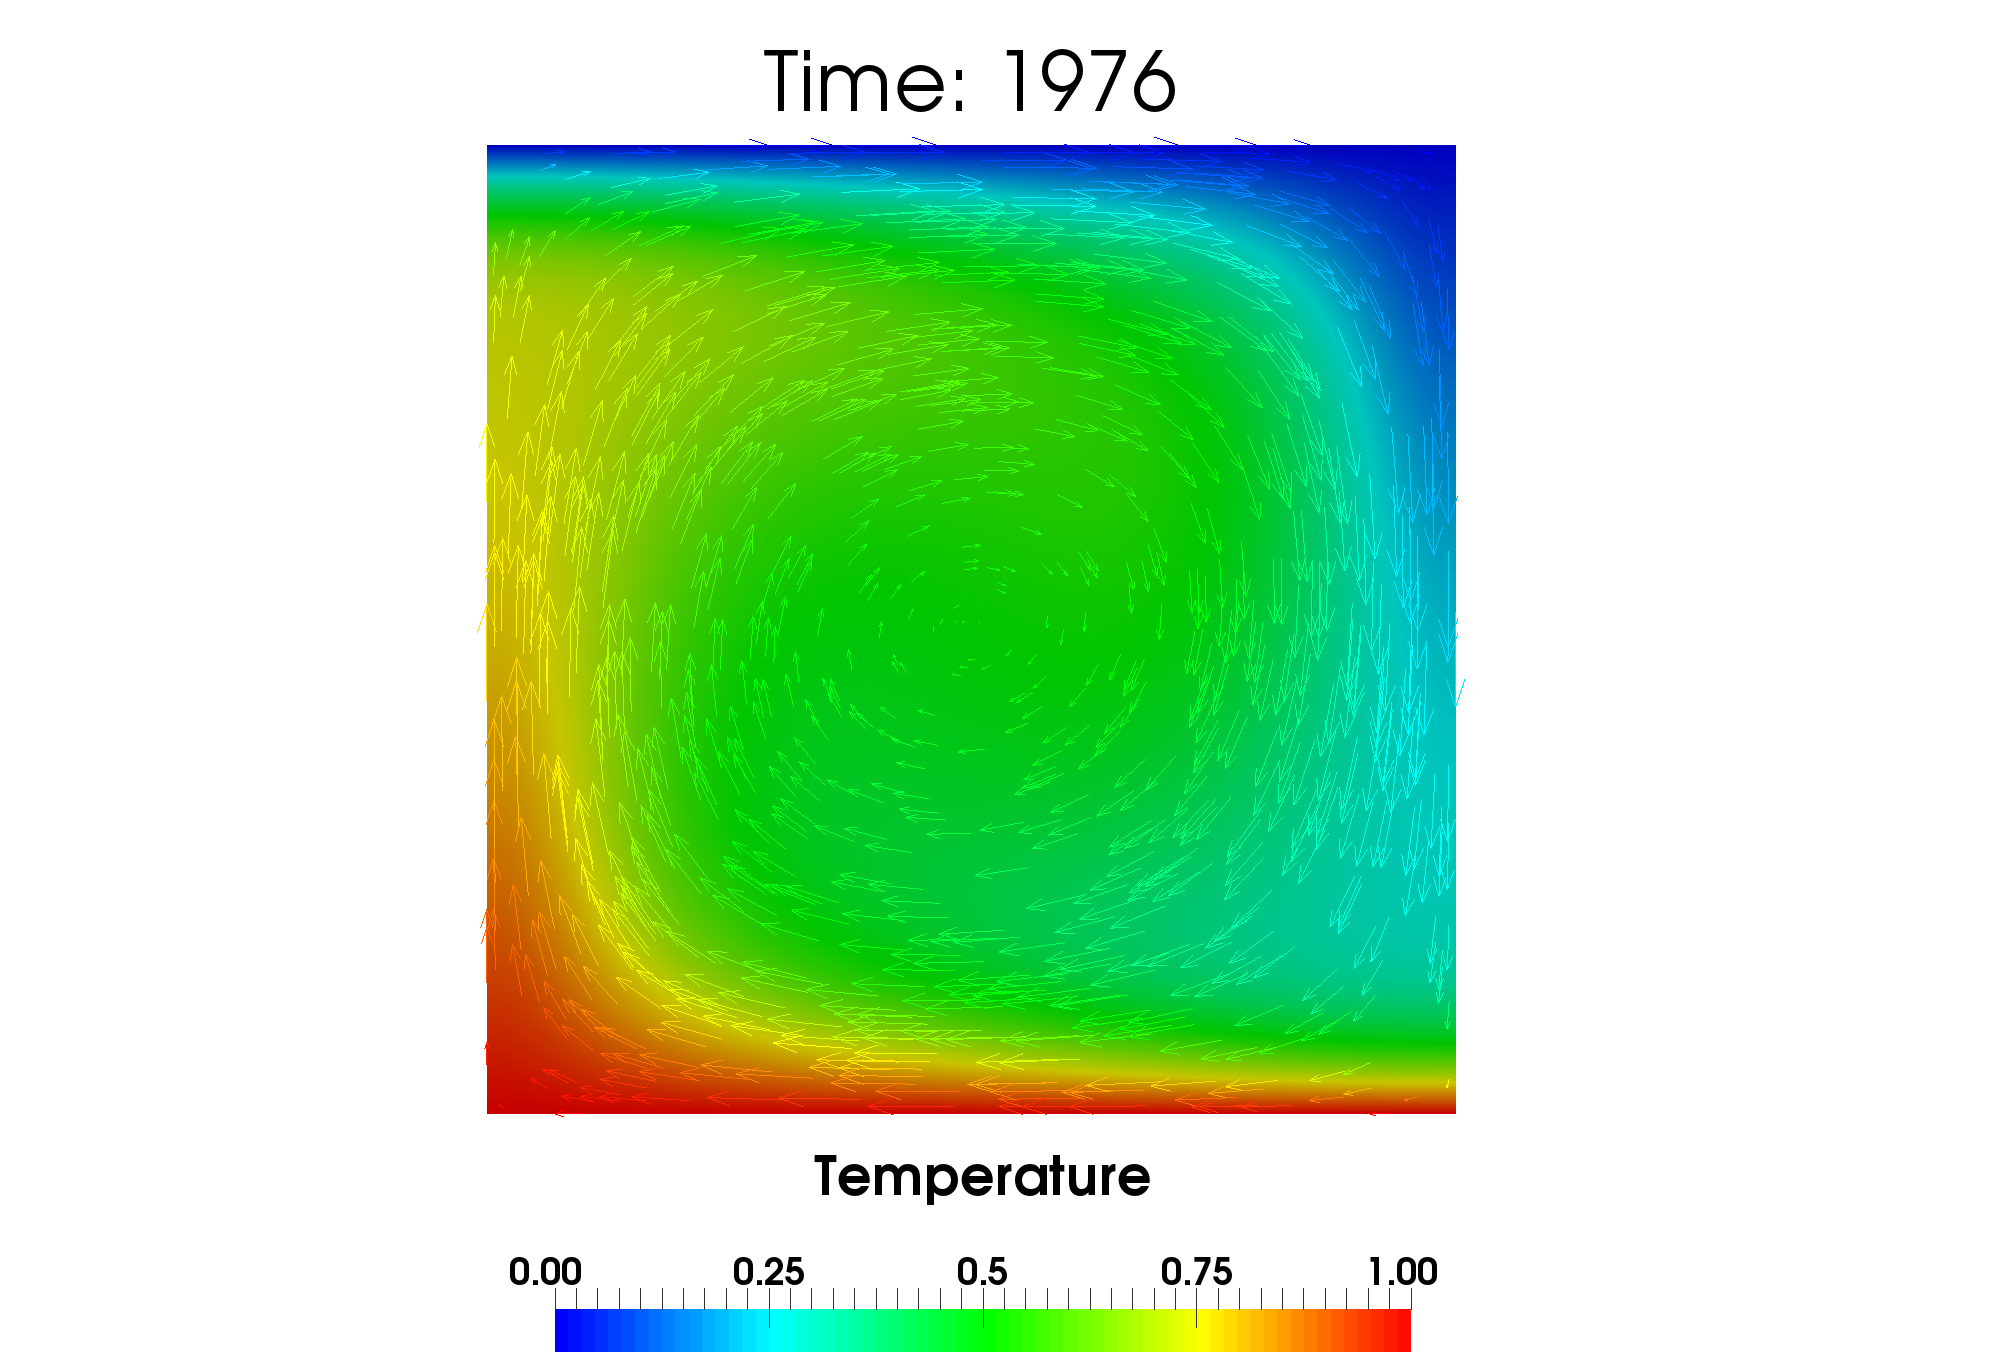
\includegraphics[width=.9\textwidth]{figures/convection_isoviscous_TV.png}
  \caption{Near-steady state solution of a simple isoviscous thermal
    convection problem Blankenbach 1a
    \cite{blankenbach_benchmark_1989} ($\Ra=10^{4}$). Resolution is
    $64\times64\times2$ triangles with mixed element
    $(v,p,T)\in([P2,P2],P1,P2])$ for 54148 total degrees of freedom.  Color field
    shows dimensionless Temperature with the velocity field shown as
    arrows. The steady state stopping criterion for this run was set
    such that all fields change by $\leq10^{-5}$ between time-steps.}
  \label{fig:convection1a}
\end{figure}

\section{Solution using \TF}

To set this problem up in \TF{}, we will reuse a large amount of the
work from our Stoke's MMS solutions but extend it to solve the
time-dependent problem.  The principal changes will be
\begin{itemize}
\setlength{\itemsep}{-.1em}
\item Set the domain to  $[0,1]\times[0,1]$ 
\item Add timestepping options including a simple adaptive time stepper.
\item Adding an additional scalar field $T\in P_{2}$ with initial and
  boundary conditions appropriate  to the system
\item Modifying the non-linear residual to the above UFL
\item Modify the solver to handle an additional field (if using
  fieldsplit block-preconditioners)
\item Adjust appropriate monitors and diagnostics
\end{itemize}

A fully worked out \texttt{tfml} file for this problem using a direct
solver for the full Jacobian (Eq. \ref{eq:4.7}) %along with a script to perform a basic convergence test
can be found in
\texttt{\$TF\_HOME/share/terraferma/tutorials/thermalconvection/ isoviscous/newton\_direct/convection.tfml}.  The
solution is shown in Figure \ref{fig:convection1a}.   




%\pagebreak{}

In more detail, the specific steps required to modify the Stokes mms
problem to solve thermal convection are as follows.
\begin{steps}{Step}
\item Make a new tfml file
  \begin{lstlisting}[style=Bash]
$ mkdir myconvection
$ cd myconvection
$ cp $TF_HOME/share/terraferma/tutorials/stokes/isoviscous/mms/mms_direct/stokes.tfml convection.tfml
$ diamond convection.tfml &
  \end{lstlisting}%$
\item \textbf{Change the geometry:} Under \texttt{geometry->Mesh},
  \begin{steps}{step}

  \item Set rectangle bounds to  $[0,1]\times[0,1]$. 
  \item increase \texttt{number\_cells} to $64\times64$
  \end{steps}
\item \textbf{Change io parameters}
  \begin{steps}{step}
  \item Change \texttt{output\_base\_name} to \texttt{rbconvection}
  \item Change \texttt{visualization->element} to (P2DG)
  \item Add appropriate dump-periods for visualization and statistics
    output.  Under \texttt{dump\_periods} do the following
    \begin{itemize}
    \item Activate \texttt{visualization\_period} and set to
      100. (i.e. output paraview files every 100 dimensionless time units)
    \item Check and output statistics every 5 time steps. Activate
      \texttt{statistics\_period}, change it to
      \texttt{statistics\_period\_in\_timesteps}, and set it to 5
    \item Check for steady state stopping criterion every 10 time
      steps. Activate \texttt{steady\_state\_period} and change it to
      \texttt{steady\_state\_period\_in\_timesteps} and set it to 10
      (i.e. check every 10 time steps  whether the change in the solution from   time-step to time-step is lower than the steady-state tolerance)
    \end{itemize}
  \end{steps}
\item \textbf{Add Time-stepping parameters}:
  \begin{steps}{step}
    \item Activate the \texttt{timestepping} tab and set the following
    \begin{itemize}
    \item \texttt{current\_time} = 0.0
    \item \texttt{finish\_time} = 1.e6
    \end{itemize}
    This will run for a dimensionless time of $10^{6}$ or until the
    solution has approached steady state (see below).
  \item \textbf{Set the time-step coefficient \texttt{dt}} Because we
    include the timestep $\Delta t$ explicitly in the form, we need to
    initialize it as a coefficient.  Unlike other coefficients, we do
    this in the Time-stepping tabs as we can add additional
    constraints such as adaptive time-stepping.
    \begin{itemize}
    \item\textbf{ Set the time-step ufl name.} Unfold\texttt{ coefficient(Timestep)} and set the
      \texttt{ufl\_symbol} to \texttt{dt}
    \item \textbf{Set the initial time-step value.}  The time step is
      of type \texttt{Constant}.  For a constant time-step just unfold the \texttt{type(Constant)} tab all the way to set
      the constant value to a fixed value.  Here however we will use
      adaptive time stepping which allows us to set the initial value
      to \textbf{0.0}. Inspection of Equation (\ref{eq:4.26}) shows that
      for \texttt{dt=0}, the problem reduces to a projection problem
      for $T_{i}$ that will simply set it to the initial condition at
      $t=0$, and then the Stoke's solver will solver for the $\vec{v}$
      and $p$ at the initial time.  After the first time-step, the
      adaptive time stepper will choose an appropriate value of
      \texttt{dt} based on a Courant condition.
    \end{itemize}
  \item \textbf{Set Adaptive Time-stepping parameters}. This problem
    will set a crude adaptive time-stepper based on a Courant number
    constraint.  In general, our constraints will
    scale with $\Delta t$, e.g. the Courant number can be considered a
    field
    \begin{displaymath}
      \alpha = \frac{\Delta t ||\vec{v}||}{h}
    \end{displaymath}
    where $h$ is a measure of the local cell-size.  Given a field
    calculated with the current time-step,  the time-stepper will
    return a modified time-step that keeps $\alpha$ to some maximum
    value (e.g. $\alpha_{max}=1$).  The actual Courant number will be calculated in a
    separate system described below.    Here we just inform TerraFERMA how the
    constraint will be implemented.  Do the following
    \begin{itemize}
    \item Activate the
    \texttt{adaptive} tab and add a \texttt{constraint} named
    \texttt{Courant}.
  \item Add the system name that calculates the constraint set
    \texttt{system = CourantNumber}
  \item Set the field or coefficient that is evaluated
    (i.e. \texttt{Field = CourantNumber}
  \item Set the maximum value of the constraint
    \texttt{requested\_maximum\_value = 2.}
  \item In addition you can set fields to determine how often the
    timestep check is called (\texttt{adapt\_period}) as well as the
    maximum amount of growth per time-step when the time-step is
    increasing.  More details on these parameters is given in the help
    windows in diamond. Here we will just check the time step every
    other step.
  \item Activate and set {adapt\_period\_in\_timesteps = 2}
    \end{itemize}
  \item \textbf{Set a steady state check:} We can also stop the
    time-loop when the change from time-step to time-step for any set
    of monitored fields drops below some tolerance.  To activate a
    steady state check
    \begin{itemize}
    \item Under \texttt{}Activate the \texttt{steady\_state} tab
    \item Set the tolerance to \texttt{1.e-5}
    \end{itemize}
    When we describe the fields below we have the option of adding
    them to the steady-state checker.
  \end{steps}
\item \textbf{Add a few global ufl parameters:}  Sometimes it is
  convenient to define a few ufl parameters that will be included in
  all forms.  Here we will just set the values of $\theta$ and
  $\theta_{v}$ that control the theta weightings for Temperature and
  Velocity and define the viscosity as constant (by putting the
  viscosity here, we can more easily modify it later to non-constant viscosity).  Do the following:
  \begin{itemize}
  \item under \texttt{global\_parameters} activate the \texttt{ufl} tab
  \item replace the (string) with the following ufl
    \begin{lstlisting}[style=UFL]
# theta weightings for Temperature and velocity
theta = 0.5
theta_v = 0.5

# scaled viscosity 
eta = 1.
    \end{lstlisting}

  \end{itemize}
\textbf{Caution:} Global ufl options should be used sparingly
  as any change to them will force a re-compile and a regeneration of
  all the ufl code.  To modify constants as run-time parameters, set
  them up as coefficients.
\item \textbf{Modify System Stokes to System Convection}
  \begin{steps}{step}
  \item \textbf{Change the system name} to  \texttt{Convection} (the \texttt{ufl\_symbol}
    remains the same, \texttt{us})
  \item \textbf{Modify Properties for Velocity}.  We will need two
    sets of boundary conditions to impose the no-flow boundaries (the
    free-stress conditions are imposed in the weak-forms), as well as
    cleaning up some of the diagnostics and setting the steady-state
    checkers.  Do the following
         \begin{steps}{do}
      \item \textbf{Set $v_{x}=0$ on the left and right boundaries}: remove (or
        edit) the existing \texttt{boundary\_condition} tab to have
        the following parameters
        \begin{itemize}
        \item \texttt{boundary\_condition} name=\texttt{LeftRight}
        \item \texttt{boundary\_ids} = 1 2
        \item \texttt{sub\_components} name = \texttt{vx}
        \item \texttt{components} = 0
        \item \texttt{type(Dirichlet)} constant = 0
        \end{itemize}
      \item \textbf{Set $v_{y}=0$ on the top and bottom boundaries}: Repeat (or use the copy paste function in diamond) to
        make a second boundary condition for the top and bottom
        boundaries
        \begin{itemize}
        \item \texttt{boundary\_condition} name=\texttt{TopBottom}
        \item \texttt{boundary\_ids} = 3 4
        \item \texttt{sub\_components} name = \texttt{vy}
        \item \texttt{components} = 1
        \item \texttt{type(Dirichlet)} constant = 0
        \end{itemize}
    \item \textbf{Turn on steady-state checking}: under
      \texttt{diagnostics}, activate the tab
      \texttt{include\_in\_steady\_state} and set the norm to be
      checked to \texttt{linf} (infinity norm)
      \end{steps}
    \item \textbf{Modify Properties for Pressure}
      \begin{itemize}
      \item Move the reference point to $[0.5, 0.5]$
      \item \textbf{Turn on steady-state checking}:  under
      \texttt{diagnostics}, activate the tab
      \texttt{include\_in\_steady\_state} and set the norm to be
      checked to \texttt{linf}
      \end{itemize}
    \item \textbf{Add a new Field and diagnostics for Temperature}.
      Activate a new field and set the following properties, BC's and IC's
      \begin{itemize}
      \item \texttt{name} = \texttt{Temperature}
      \item \texttt{ufl\_symbol (global)} = T
      \item \textbf{Set properties of the \texttt{type(Function)}}
        \begin{steps}{do}
        \item set \texttt{rank(Scalar)}
        \item set \texttt{element(P2)}
        \item set the initial condition
          \begin{displaymath}
            T = 1. - y + 0.2\cos(\pi x)\sin(\pi y)
          \end{displaymath}
using the python Expression
\begin{lstlisting}[style=python]
def val(x):
  from math import sin, cos, pi
  return 1.-x[1] + 0.2*cos(x[0]*pi)*sin(x[1]*pi)
\end{lstlisting}
\item \textbf{Set the Dirichlet boundary condition on the top $T=0$}
  \begin{itemize}
  \item activate a new \texttt{boundary\_condition} tab and name it \texttt{Top}
\item set \texttt{boundary\_ids} = 4
\item set \texttt{sub\_components(All)} $\rightarrow$
  \texttt{type(Dirichlet)}$\rightarrow$ \texttt{constant} =0.0
  \end{itemize}
\item \textbf{Set the Dirichlet boundary condition on the bottom $T=1$}
  \begin{itemize}
  \item activate (or copy) a new \texttt{boundary\_condition} tab and name it \texttt{Bottom}
\item set \texttt{boundary\_ids} = 3
\item set \texttt{sub\_components(All)} $\rightarrow$
  \texttt{type(Dirichlet)}$\rightarrow$ \texttt{constant} =1.0
  \end{itemize}
\item \textbf{Set appropriate Diagnostics for Temperature}:  Here we
  should add to visualization, statistics and steady-state monitoring
  \begin{itemize}
  \item activate \texttt{include\_in\_visualization}
  \item activate \texttt{include\_in\_statistics}. 
\item activate \texttt{include\_in\_steady\_state} and set the norm
  type to \texttt{linf}
  \end{itemize}
        \end{steps}
      \end{itemize}

    \item \textbf{remove the coefficients} for \texttt{AnalyticVelocity},
      \texttt{AnalyticPressure}, and \texttt{src}.
    \item \textbf{Add a new coefficient for the Rayleigh Number}
      \begin{itemize}
      \item set the \texttt{name} = \texttt{RayleighNumber}
      \item set the \texttt{ufl\_symbol (global)} = \texttt{Ra}
      \item set
        \texttt{type(Constant)}$\rightarrow$\texttt{rank(Scalar)}$\rightarrow$\texttt{value(WholeMesh)}$\rightarrow$\texttt{constant}
        = \texttt{1.e4}
      \end{itemize}
    \item \textbf{Update the non-linear solver for convection}
    \begin{steps}{do}
    \item Change the residual from Stokes to full   thermal convection
      by adding the temperature residual i.e. implement the ufl
      described above 
\pagebreak{}
    \begin{lstlisting}[style=UFL]
# theta weighted variables
T_theta = theta*T_i + (1.-theta)*T_n
v_theta = theta_v*v_i + (1.-theta_v)*v_n

# Velocity, Pressure and Temperature residuals
Fv = (inner(sym(grad(v_t)), 2.*eta*sym(grad(v_i))) - 
        div(v_t)*p_i - T_i*v_t[1])*dx
Fp = -p_t*div(v_i)*dx
FT = (T_t*((T_i - T_n) + dt*inner(v_theta, grad(T_theta))) + 
         dt/Ra*inner(grad(T_t), grad(T_theta)))*dx

# Total non-linear residual for the system
F = Fv + Fp + FT
    \end{lstlisting}
  \item \textbf{Change the SNES type to ls}:  This is real newton now
    and you'll need a real non-linear solver.
  \item \textbf{Keep a direct solver for Newton (for the moment)}.  A
    sparse direct solve for the full $3\time3$ block Jacobian is
    inefficient and we will change it shortly to a
    block-preconditioned iterative solver, but for now we'll keep the
    sparse direct solver and use it as a base-line case.
    \end{steps}
  \item \textbf{Use the solver at every time step:} change
    \texttt{solve(at\_start)} to \texttt{solve(in\_timeloop)}
  \item \textbf{Modify/Add some Functionals}
    \begin{itemize}
    \item Remove the functionals \texttt{VelocityL2NormSquared},
      \texttt{VelocityL2NormErrorSquared},
      \texttt{PressureL2NormSquared} and
      \texttt{PressureL2ErrorNormSquared}
    \item \textbf{Add a functional for the Nusselt Number}
      \begin{itemize}
      \item set the \texttt{name = TemperatureNu}
      \item set the \texttt{ufl\_name (functional) = int}
      \item add the ufl
       \begin{lstlisting}[style=UFL]
         int = -T.dx(1)*ds(4)
       \end{lstlisting}
 which will calculate the integral of the heat-flux ($-\nabla T\cdot
 \hat{n}$) across the top boundary.
\end{itemize}
\item \textbf{Add a functional for the rms variation in velocity}
      \begin{itemize}
      \item set the \texttt{name = VelocityvrmsSquared}
      \item set the \texttt{ufl\_name (functional) = int}
      \item add the ufl
       \begin{lstlisting}[style=UFL]
int = Ra*Ra*inner(v,v)*dx
       \end{lstlisting}
 which will calculate the integral of the magnitude squared of the velocity
 field over the domain.  The $\Ra^{2}$ scaling is to make this number
 comparable to the numbers used in \cite{blankenbach_benchmark_1989}.
      \end{itemize}
    \end{itemize}
\end{steps}
  \item \textbf{Add a new system to calculate the Courant Number}.  To
    implement our adaptive time-stepper we need to also calculate a
    field of courant numbers for every cell.
    \begin{steps}{step}
    \item \textbf{Activate a new System} 
      \begin{itemize}
      \item set the \texttt{name = CourantNumber}
      \item choose \texttt{mesh (Mesh)}
      \item set the \texttt{ufl\_name (global) = uc}
      \end{itemize}
    \item \textbf{Activate a new field: CourantNumber} and unfold
     \begin{itemize}
      \item set the \texttt{name = CourantNumber}
      \item set the \texttt{ufl\_name (global) = c}
      \item Under \texttt{type(Function)}
        \begin{itemize}
        \item choose \texttt{rank (Scalar)}
        \item choose \texttt{element (P0)}. We will calculate a
          constant value of $\alpha$ for each cell.
        \item set \texttt{initial\_condition}$\rightarrow$\texttt{constant = 0.}
        \end{itemize}
      \item If you want, \textbf{activate diagnostics} for
        \texttt{include\_in\_visualization}, \texttt{include\_in\_statistics}
      \end{itemize}
      
    \item \textbf{Activate a new Solver}
\begin{itemize}
      \item set the \texttt{name = Solver}
      \item choose \texttt{type (SNES)}
      \item \textbf{set the Residual}
        \begin{itemize}
        \item set the ufl 
\begin{lstlisting}[style=UFL]
# Finite volume style estimate of Courant number
# calculate the outward facing normal component of velocity for each facet
n = FacetNormal(c_e.cell())
vn = dot(v_i, n)
vout = 0.5*(vn + abs(vn))

# project the cell integral of the the outgoing flux from each cell
F = c_t*c_i*dx - 
      c_t('+')*vout('+')*dt('+')*dS - c_t('-')*vout('-')*dt('-')*dS - 
      c_t*vout*dt*ds(1) - c_t*vout*dt*ds(2) - 
      c_t*vout*dt*ds(3) - c_t*vout*dt*ds(4)
    \end{lstlisting}
which is the weak form for $\alpha$ that depends on the timestep
$\Delta t$ and integral of the outgoing flux through each cell. \textbf{CAUTION!}
 if you copy and paste the above UFL from the pdf manual to diamond,
 you will introduce some non-ascii characters into the ufl that will
 break FFC.  In this case,  the single quote character \texttt{'} will need to
 be edited to a standard ascii single quote.
\item set the residual \texttt{ufl\_symbol (solver) = F}
\end{itemize}
\item \textbf{Set the Jacobian}
\begin{itemize}
\item set the ufl 
\begin{lstlisting}[style=UFL]
J = derivative(F,uc_i,uc_a)
    \end{lstlisting}
\item set \texttt{ufl\_symbol (solver) = J}
        \end{itemize}
      \item Set \texttt{relative\_error = 1.e-6}
      \item Set \texttt{max\_iterations = 1}

      \item Set the Linear solver
        \begin{itemize}
        \item Choose \texttt{iterative\_method (preonly)}
        \item Choose \texttt{preconditioner (Jacobi)} (the mass matrix
          for a P0 function is exactly diagonal)
        \end{itemize}
      \item Choose \texttt{solve\_with\_diagnostics} to evaluate the
        courant number only at diagnostics (or whenever the adaptive
        time-stepper is called)
        \end{itemize}

   \end{steps}
  \item \textbf{Test the build using}
   \begin{lstlisting}[style=Bash]
$ tfbuild convection.tfml
$ cd build
$ make -j 3
$ make run
   \end{lstlisting}
or copy the testharness file \texttt{convection.shml} from
\texttt{\$TF\_HOME/tutorials/thermalconvection/isoviscous/newton\_direct}
to your current working directory and run
\begin{lstlisting}[style=Bash]
  $ tfsimulationharness --test convection.shml 
\end{lstlisting}
%$
although you might need to edit it for name consistency.

\end{steps}


%\pagebreak{}
\section{Themes and Variations}

Many of the simple variations demonstrated in Chapter
\ref{cha:stokes-equation} for Stoke's  are readily adapted
to the thermal convection problem.  In particular, we can try many
variations on the fieldsplit block pre-conditioners.

\subsection{Iterative Solvers and Fieldsplit preconditioners}

The previous problem uses a sparse-direct solver on the full
$3\times3$ block Jacobian given by Eq. (\ref{eq:4.7}).  While this is
expected to give optimal convergence of the non-linear problem, these
large coupled systems can be expensive to assemble and solve. However,
\TF{} provides many options for exploring and tuning more efficient
methods that can balance convergence and performance.  For example,we
could also use a physically motivated approximate Jacobian
\begin{equation}
  \label{eq:4.9}
   P = \left[
\begin{array}{ccc}
  K & G  & M \\
  G^{T} & 0 & 0 \\
  0 & 0 & A \\ 
  \end{array}
  \right].
\end{equation}
instead of the full Jacobian $J$. $P$ simply neglects the coupling between temperature and velocity
(by  assuming that $B=0$).  In this case, $P$ is block
upper-triangular such that $P\delta = -\vec{F}$  can be solved
sequentially by first solving for the Temperature correction $\delta
T_{i}$ using
\begin{equation}
  \label{eq:4.14}
  A(\vec{v}_i)\delta T_i = -F_{T}(\vec{u}_i)
\end{equation}
using the previous value for $\vec{v}_i$, then updating the velocity field by solving the linear
Stokes system
\begin{equation}
  \label{eq:4.8}
   \left[
\begin{array}{cc}
  K & G  \\
  G^{T} & 0 \\
  \end{array}
  \right]
  \left[
    \begin{array}{c}
      \vec{\delta v}_i \\
      \delta p_i \\
    \end{array}
  \right] = -\left[
    \begin{array}{c}
      F_{\vec{v}}(\vec{u}_{i}) + M\delta T_{i}\\
      F_p(\vec{u}_{i})\\
    \end{array}
  \right]
\end{equation} .


If we just use $P$ as an approximate Jacobian in a Newton scheme, it
can be shown that if the  viscosity is independent of $T$, this
algorithm is equivalent to a standard Picard splitting which first
solves for the  Temperature field with the current velocity,  then
solves for the velocity with the new temperature,  iterating until
some stopping criteria. However,  if we use $P$ as a
\emph{preconditioner} for solving the exact problem
$J\vec{\delta}=-\vec{F}$ using the full Jacobian,
Eq. (\ref{eq:4.7})  we can  get the expected quadratic
convergence of newton with the computational expense of a Picard
iteration.

Figure \ref{fig:isoviscous_conv_perf} compares the
convergence behavior for four solver strategies 
\begin{description}
\item[newton\_direct]  sparse direct solver on $J$
\item[preonly\_fieldsplit\_direct] Just apply the  preconditioner $P$,
  fieldsplit between $T$ and
  $(\vec{v},p)$ using sparse direct
  solvers on the $A$ and Stokes blocks.  This method is equivalent to solving an approximate Newton
  iteration replacing $J$ with $P$.
\item[newton\_fieldsplit\_direct]  Solve $J\vec{\delta}=-F$ using
  flexible gmres, preconditioned by fieldsplit $P$.
\item[picard\_splitting] Solve two systems sequentially, first solving
  for $T$, then Stokes for $(\vec{v},p)$ and iterating until converged.
\end{description}
All schemes were run until $||F||_{2}<10^{-11}$.  

\begin{figure}[htb]
  \centering
\includegraphics[width=0.5\textwidth]{figures/Solver_comparison_SNES_convergence_isoviscous.pdf}\hfill{}
\includegraphics[width=0.5\textwidth]{figures/Solver_comparison_Walltime_isoviscous.pdf}\\
\caption{Comparison of convergence behavior and performance for a
  range of preconditioner-solver options for isoviscous thermal
  convection (Figure \ref{fig:convection1a}).  (\textbf{a})
  convergence behavior of different solver schemes at time-step 9
  showing linear convergence for picard\_splitting and
  preonly\_fieldsplit\_direct (which are identical) and quadratic convergence for
  two Newton schemes   newton\_direct and newton\_fieldsplit\_direct. (\textbf{b}) relative
  performance of the different solver schemes shown as total walltime
  normalized by the maximum time for newton\_direct.  For this problem
the fieldsplit block-preconditioned Newton schemes is $\sim2.5$ times
faster than newton or Picard.}
  \label{fig:isoviscous_conv_perf}
\end{figure}

As expected, Picard splitting and the approximate newton scheme show
the same convergence behavior with $\sim$ 5 non-linear iterations
required for convergence.  Newton\_direct and
newton\_fieldsplit\_direct show quadratic convergence and converge in
2 iterations. 

In terms of performance, however, newton\_direct is more expensive due
to the significantly larger matrix factorization of $J$.  For this
problem, at any rate,  newton\_fieldsplit\_direct is two
times$\sim2.5$ times  faster than both direct Newton and Picard as it has combines the
computational cost of the Picard iteration with much faster
convergence. 


\subsubsection*{Implementation in \TF}
\label{sec:implementation-tf}

Implementing the different solver strategies in \TF{} is relatively
straightforward. Fully worked out examples can be found in the
subdirectories of
\texttt{\$TF\_HOME/share/terraferma/tutorials/thermalconvection/isoviscous}. All
four simulations can be run and Figure \ref{fig:isoviscous_conv_perf}
generated using
\begin{lstlisting}[style=Bash]
  $ tfsimulationharness --test compare_solvers
\end{lstlisting} %$
\textbf{Note}: If you are fortunate to have a multi-core server you
can speed this up significantly by running the four simulations
simultaneously using 
\begin{lstlisting}[style=Bash]
  $ tfsimulationharness --test -n 4 compare_solvers
\end{lstlisting} %$
where \texttt{-n 4} indicates 4 threads.

In more detail, the specific solver setting for the four different
strategies are
\begin{description}
\item[newton\_direct] Under \texttt{nonlinear\_solver
    (Solver)}$\rightarrow$\texttt{type (SNES)}$\rightarrow$\texttt{linear\_solver}
  \begin{itemize}
  \item set \texttt{iterative\_method (preonly)}
  \item set \texttt{preconditioner (lu)} 
  \item choose your favorite
    sparse-direct solver (e.g. \texttt{umfpack} or \texttt{mumps})
  \end{itemize}
\item[preonly\_fieldsplit\_direct] Under \texttt{nonlinear\_solver
    (Solver)}$\rightarrow$\texttt{type (SNES)} $\rightarrow$ \texttt{linear\_solver}
  \begin{itemize}
  \item set \texttt{iterative\_method (preonly)}
  \item set \texttt{preconditioner (fieldsplit)}
    \begin{itemize}
    \item set \texttt{composite\_type (multiplicative)}\footnote{a
        multiplicative fieldsplit preconditioner uses the results of
        previous block solves as they become available.  Thus the
        order of splits is important.  If we solve $T$ then Stokes,
        the preconditioner is upper triangular, otherwise it's lower
        triangular.  A \texttt{composite\_type (additive) is just
          block diagonal}}
    \item Now set the individual fieldsplits and solvers for each
      split.  Here we will have two splits.  The first for Temperature
      $T$, and the second for Stokes $(\vec{v},p)$. We will use sparse
      direct solvers for each of the splits. In detail
      \begin{itemize}
      \item Activate a fieldsplit and set the name to
        \texttt{Temperature}.  Beneath this
        \begin{itemize}
      \item activate a field named
        \texttt{Temperature}
      \item Set the \texttt{linear\_solver} to
        \texttt{iterative\_method (preonly)}  and
        \texttt{preconditioner (lu)}
      \end{itemize}
      \item Activate another fieldsplit and set the name to
        \texttt{Stokes}. Beneath this
        \begin{itemize}
      \item activate a field named  \texttt{Pressure}
      \item activate a field named  \texttt{Velocity}
      \item Set the \texttt{linear\_solver} to
        \texttt{iterative\_method (preonly)}  and
        \texttt{preconditioner (lu)}
      \end{itemize}

      \end{itemize}
    \end{itemize}
  \end{itemize}
\item[newton\_fieldsplit\_direct] Under \texttt{nonlinear\_solver
    (Solver)}$\rightarrow$\texttt{type (SNES)} $\rightarrow$ \texttt{linear\_solver}
  \begin{itemize}
  \item just set \texttt{iterative\_method (fgmres)}
  \item set \texttt{preconditioner (fieldsplit)} and use all the
    fieldsplit options from the previous example.
\end{itemize}
\item[picard\_splitting] \TF{} also allow implementation of more
  classical Picard Splitting schemes for this problem that split the
  problem over two separate systems, one for Temperature, the other
  for Stokes, then solves them sequentially using the output of one
  system as coefficients in the other, but calculating the non-linear
  residual of the entire system $F(T,\vec{v},p)$ at each iteration
  until convergence.  The input file
  \texttt{picard\_splitting/convection.tfml} implements this
  approach.  The key differences that need to be implemented are
  \begin{itemize}
  \item activate \texttt{nonlinear\_systems} (greyed out below
    \texttt{timestepping} options), and set
    \begin{itemize}
    \item \texttt{relative\_error = 1.e-8}
    \item \texttt{absolute\_error = 1.e-11}
    \item \texttt{max\_iterations = 20}
    \item and any monitors of interest
    \end{itemize}
  \item Add or copy a system to just solve Temperature such that
    \begin{itemize}
    \item \texttt{ system name = Temperature}
    \item \texttt{ufl\_symbol (global) = uT}
    \item has a single \texttt{field (Temperature)} with the same BC's
      and IC's as before
    \item Solver settings
      \begin{itemize}
      \item \texttt{Residual}
        \begin{lstlisting}[style=ufl]
T_theta = theta*T_i + (1.-theta)*T_n
v_theta = theta_v*v_i + (1.-theta_v)*v_n

F = (T_t*((T_i - T_n) + dt*inner(v_theta, grad(T_theta))) +
       dt/Ra*inner(grad(T_t), grad(T_theta)))*dx
        \end{lstlisting}
\item \texttt{Jacobian}
        \begin{lstlisting}[style=ufl]
J = derivative(F, uT_i, uT_a)
        \end{lstlisting}
      \end{itemize}
    \item Set linear solver to \texttt{iterative\_method (preonly)},
      \texttt{preconditioner (lu)}
    \item Add any functionals of interest

    \end{itemize}

  \item Add a system to just solve Stokes.
    \begin{itemize}
    \item \texttt{ system name = Convection} (or Stokes?)
    \item \texttt{ufl\_symbol (global) = us}
    \item two fields \texttt{field (Pressure)} and \texttt{field
        (Velocity)} each  with the same BC's
      and IC's as before
    \item Solver settings
      \begin{itemize}
      \item \texttt{Residual}
        \begin{lstlisting}[style=ufl]
Fv = (inner(sym(grad(v_t)), 2.*eta*sym(grad(v_i))) - 
         div(v_t)*p_i - T_i*v_t[1])*dx
Fp = -p_t*div(v_i)*dx

F = Fv + Fp          
        \end{lstlisting}
\item \texttt{Jacobian}
        \begin{lstlisting}[style=ufl]
J = derivative(F, us_i, us_a)
        \end{lstlisting}
      \end{itemize}
    \item Set linear solver to \texttt{iterative\_method (preonly)},
      \texttt{preconditioner (lu)}
    \item Add any functionals of interest
    \end{itemize}
  \end{itemize}
\end{description}




\subsection{Variable Viscosity}
\label{sec:variable-viscosity}

The previous example demonstrates the flexibility of \TF{} to readily
compose and compare different solver strategies.  This ability becomes
even more important for strongly coupled non-linear problems.  For
example, Figure \ref{fig:convectionTVdepVisc} shows a convection
calculation with a more realistic temperature and strain-rate
dependent composite rheology
\begin{equation}
  \label{eq:4.10}
  \eta(T,V) =
  \left[
\frac{1}{\eta_{\text{diff}}} + \frac{1}{\eta_{\text{disl}}} + \frac{1}{\eta_{\text{max}}}
  \right]^{-1}
\end{equation}
where
\begin{align}
  \label{eq:4.11}
  \eta_{diff} = &A_{\text{diff}}\exp
  \left[
\frac{E_{diff}}{RT}
  \right]\\
\eta_{disl} =& A_{\text{disl}}\exp
\left[
\frac{E_{disl}}{nRT}
\right]\tilde{\dot{\epsilon}}_{II}^{1/n -1}\\
\eta_{max} =& 10^{24} ~\mathrm{\,Pa\,\, s}
\end{align}
are appropriate (dimensional) rheologies for diffusion creep,
dislocation creep and a viscosity cap \cite{billen_rheologic_2007}.
These rheologies are readily incorporated directly into the ufl and
are included in all the problems with the
\texttt{global\_parameters}$\rightarrow$\texttt{ufl} field as
\begin{lstlisting}[style=ufl]
# model parameters for determining viscosities
v0    =  Ra*kappa/h             # reference advection velocity m/s
edot0 = (v0/h)                  # scaled strainrate

# definition of strain rate tensor and second invariant
edot = sym(grad(v_i))
eIIreg = sqrt(0.5*(inner(edot,edot) + epssquared))

# dimensional temperature
T0 = 873.00                     # Moho Temperature
delta_T = 1500.00               # temperature difference across system
Tdim = delta_T*T_i + T0          

# inverse  viscosities
A1 = 7573290518.9976 #(eta0/Adiff)
A2 = -26.860705193737846  #-Ediff/R/delta_T
T0p = 873./1500
B1 =  34520.1355950926     # (eta0/Adisl)*(edot0)**inexp
B2 =  -12.37081518517564   # -Edisl/(stressn*R*delta_T)
ietamax = 1.e-5
inv_etadiff = A1*exp(A2/(T_i + T0p))  # scaled inv diffusion creep
inv_etadisl = B1*exp(B2/(T_i + T0p))*(eIIreg**inexp) # scaled inv dislocation creep
# scaled inverse viscosity
inv_etaprime = inv_etadiff + inv_etadisl + ietamax

eta = 1./inv_etaprime
\end{lstlisting}
Here, many of the constant have been hardwired into the ufl, however,
it is generally better to include the constants as coefficients and
control them through the simulation testharness.

In this case the full problem is considerably more non-linear.  In
particular, the Stokes sub-problem is now fully non-linear due to the
dependence of viscosity on the strain-rate tensor through
\begin{equation}
\tilde{\dot{\epsilon}}_{II} = \sqrt{\frac{\dot{\epsilon}(\vec{v}):\dot{\epsilon}(\vec{v}) + \dot{\epsilon}_{\varepsilon}}{2}}
\end{equation}
where we have regularized the second invariant (of the
\emph{dimensionless} velocities) by
$\dot{\epsilon}_{\varepsilon} = 2\times10^{-10}$ to prevent
singularities in the Jacobian at low strain-rates.

The Jacobian matrix, which may again be calculated by automatic differentiation, is still block structured:
\begin{equation}
  \label{eq:TVJacobian}
  J =  \left[
\begin{array}{ccc}
  \left[K + \eta_{\vec{v}}\right] & G  & \left[M + \eta_{T}\right] \\
  G^{T} & 0 & 0 \\
  B & 0 & A \\ 
  \end{array}
  \right]
\end{equation}
but with additional coupling blocks, $\eta_{\vec{v}}(\vec{u}_i)$ and $\eta_{T}(\vec{u}_i)$ due to the variation of viscosity with velocity
and temperature respectively which also make $K(\vec{u}_i)$ non-linear.  
\begin{figure}[htbp!]
  \centering
  \includegraphics[width=.9\textwidth]{figures/convection_TVdependent_TV.png}
  \caption{Solution of a thermal convection problem with Temperature
    and strainrate dependent viscosity (Eq.~\ref{eq:4.10}) and  nominal Rayleigh Number
    $\Ra=10^{4}$. Numerical parameters and resolution are the same as
    in Figure \ref{fig:convection1a}. Color field shows dimensionless
    Temperature with the velocity field shown as arrows. This model is   described in
    \texttt{\$TF\_HOME/share/terraferma/tutorials/thermalconvection/TVdependentViscosity}
  and demonstrates a stagnant lid and considerably assymetry in flow}
  \label{fig:convectionTVdepVisc}
\end{figure}

\begin{figure}[htb]
  \centering
\includegraphics[width=0.49\textwidth]{figures/Solver_comparison_SNES_convergence_TVvisc.pdf}\hfill{}
\includegraphics[width=0.49\textwidth]{figures/Solver_comparison_Walltime_TVvisc.pdf}\\
  \caption{Comparison of convergence behavior and performance for a
    range of preconditioner-solver options for  the thermal
    convection problem shown in Figure \ref{fig:convectionTVdepVisc}.  
    (\textbf{a}) convergence behavior of different solver
    schemes at time-step 27 showing linear convergence for
    \texttt{picard\_splitting} and \texttt{preonly\_fieldsplit\_direct}
    and quadratic for \texttt{newton\_direct} and
    \texttt{newton\_fieldsplit\_direct}. An approximate Jacobian shows
    a convergence pattern part-way between linear and quadratic. (\textbf{b}) relative
    performance of different solver schemes normalized by the total
    walltime for \texttt{newton\_direct}. Note: the extra assembly and
    solution    time of the full Jacobian $J$ offsets its gains in
    convergence.  However using an approximate Jacobian that maintains
    the non-linearity in Temperature but not in Velocity performs best
  at near 3 times \texttt{newton\_direct}.  These figures can be
  recreated by running \texttt{tfsimulationharness --test
    compare\_solvers.shml} within the \texttt{TVDependentViscosity} directory.}
  \label{fig:Tvdependentvisc_conv_perf}
\end{figure}

 




Figure \ref{fig:Tvdependentvisc_conv_perf} shows convergence and performance results for the same solver strategies discussed for the
isoviscous case: \texttt{newton\_direct},
\texttt{preonly\_fieldsplit\_direct},
\texttt{newton\_fieldsplit\_direct}, and \texttt{picard\_splitting}
Unlike the isoviscous case, \texttt{preonly\_fieldsplit\_direct} and
\texttt{picard\_splitting} are no longer equivalent. 
% The first
% successively solving
% \begin{equation}
%   \label{eq:TVapproxnewtonsteps}
%   A(\vec{v}_i)\delta T_i = -r_{T}(\vec{u}_i) \quad \textrm{then} \quad
%    \left[
% \begin{array}{cc}
%   \left[K(\vec{u}_i) + K_{\vec{v}}(\vec{u}_i)\right] & G  \\
%   G^{T} & 0 \\
%   \end{array}
%   \right]
%   \left[
%     \begin{array}{c}
%       \vec{\delta v}_i \\
%       \delta p_i \\
%     \end{array}
%   \right] = -\left[
%     \begin{array}{c}
%       r_{\vec{v}}(\vec{u}_i) + \left[M+K_T(\vec{u}_i)\right]\delta T_i\\
%       r_p(\vec{u}_i)\\
%     \end{array}
%   \right]
% \end{equation}
% and the second
% \begin{equation}
%   \label{eq:TVpicardsteps}
%   A(\vec{v}_i)\delta T_i = -r_{T}(\vec{u}_i) \quad \textrm{then} \quad
%    \left[
% \begin{array}{cc}
%   K(\vec{u}_{i+1/2}) & G  \\
%   G^{T} & 0 \\
%   \end{array}
%   \right]
%   \left[
%     \begin{array}{c}
%       \vec{\delta v}_i \\
%       \delta p_i \\
%     \end{array}
%   \right] = -\left[
%     \begin{array}{c}
%       r_{\vec{v}}(\vec{u}_{i+1/2})\\
%       r_p(\vec{u}_{i+1/2})\\
%     \end{array}
%   \right].
% \end{equation}
% Due to the non-linearity of $K(\vec{u}_i)$ and $K_{\vec{v}}(\vec{u}_i)$, $r_{\vec{v}}(\vec{u}_{i+1/2})$ is no longer equivalent to
% $r_{\vec{v}}(\vec{u}_i) + \left[M+K_T(\vec{u}_i)\right]\delta T_i$. 
However, their convergence behaviors are similar with only
marginal gains seen using the approximate Newton scheme.  As before
the full benefits of Newton's method are only seen
using \texttt{newton\_direct} and \texttt{newton\_fieldsplit\_direct},
where the norm of the residual drops $\sim 7$ orders of magnitude in 2
as opposed to 4 iterations.  These higher
convergence rates however come at a higher cost than using
\texttt{picard\_splitting} (see Figure
\ref{fig:Tvdependentvisc_conv_perf}), owing to the increased
computational expense  of assembling and solving the $\eta_{\vec{v}}$
and $\eta_{T}$ blocks in the full Jacobian (Eq.\ \ref{eq:TVJacobian}). 

The above discussion is not intended to be an exhaustive study of
solver strategies for thermal convection, and many more alternatives
are possible.  For example, Figure
\ref{fig:Tvdependentvisc_conv_perf} also shows results for an iterative
Newton scheme, \texttt{newton\_fieldsplit\_direct\_approx} that uses an approximate Jacobian   that maintains the
non-linearity in temperature but does not assemble the
$K_{\vec{v}}$ block in Eq.\ (\ref{eq:TVJacobian}). The only
substantive change from \texttt{newton\_fieldsplit\_direct} is in the
ufl for the residual, which is now
\pagebreak{}
\begin{lstlisting}[style=ufl]
# velocity residual and derivative, viscosity block
rv_v = inner(sym(grad(v_t)), 2.*eta*sym(grad(v_i)))*dx

# remainder of the velocity residual rv = rv_v + rv_r
rv_r =  -(div(v_t)*p_i + T_i*v_t[1])*dx

r_r = rv_r + rp + rT

# approximate Jacobian including derivative of viscosity 
#with respect to T but not V
J = derivative(r_r, us_i, us_a) + 
      inner(sym(grad(v_t)), 2.*eta*sym(grad(v_a)))*dx + 
      derivative(rv_v,(T_i),(T_a))
  
\end{lstlisting}
This scheme has both better convergence and performance than Picard
splitting, \emph{for this particular problem}, where it seems that
most of the solution is actually the diffusion creep regime, so
neglecting the some of the non-linearity due to strain-rate may be an
effective strategy.  More importantly,  these
examples demonstrate, optimal solver strategies can be highly problem
dependent and the flexibility inherent in \TF{} can greatly
facilitate exploring and implementing them.  Again nearly all of this
functionality is inherited from the two core libraries FEniCS and
PETSc, however, \TF{} provides a more uniform and flexible interface
for constructing applications from these libraries.
 


%%% Local Variables: 
%%% mode: latex
%%% TeX-master: "tftutorials"
%%% End: 

\chapter{Magma Dynamics: porosity waves}
\label{cha:porosity-waves}

\section{Problem Overview}
\label{sec:porosity_waves-formulation}


While many modeling packages in Earth science solve for thermal or
thermo-chemical convection,  one of the strengths of \TF{} is that it
is not a ``convection code'', but rather a general finite element PDE
solver and can be used to model arbitrary problems as long as the weak
forms are well posed.  In particular,  \TF{} was primarily designed to
explore coupled fluid/solid mechanics with a primary application area
being the flow of magma and fluids in the deep earth.  A more general
theory of magma dynamics has been derived by multiple authors
\cite{mckenzie_generation_1984,scott_magma_1984,scott_magma_1986,spiegelman_flow_1993,spiegelman_flow_1993-1,bercovici_two-phase_2001-1,bercovici_energetics_2003,simpson_multiscale_2010,simpson_multiscale_2010-1}
that considers the flow of a low viscosity fluid in a viscously
deformable solid matrix.  From the beginning of magma dynamics,  one
of the intriguing features of these models is that they admit
dispersive non-linear magmatic
solitary  waves that propagate through the solid as ``hump
shaped'' blobs with radial symmetry that propagate at a characteristic
speed $c$ that depends on amplitude, dimension and material
parameters.  Figure \ref{fig:SolitaryWavesAllD} shows some example
solitary wave profiles for 1,2 and 3-D solitary waves that all
propagate at the same speed $c=5$ times the melt velocity in the
background constant porosity region.  

\begin{figure}[htb!]
  \centering
  \includegraphics[width=.8\textwidth]{figures/CompositeSolitaryWaves.pdf} 
  \caption{example 1,2 and 3-D magmatic solitary waves that all move
    at speed $c=5$ times the background porosity.}
  \label{fig:SolitaryWavesAllD}
\end{figure}

In the limit of small porosity, the dimensionless governing equations for evolution
of porosity $\phi$ and ``compaction pressure'' $\pcmp$ in a frame
moving at a constant velocity $\Vs$ can be written
\begin{gather}
  \ppt{\phi} + \Vs\cdot\grad\phi = 
  \left(
    \frac{h}{\delta}
  \right)^{2}\frac{\pcmp}{\zeta}  \label{eq:5.1}\\
-\div K \grad\pcmp + \left(
    \frac{h}{\delta}
  \right)^{2}\frac{\pcmp}{\zeta} = \div K \ghat    \label{eq:5.2}
\end{gather}
where $K=\phi^{n}$ is the permeability, $\zeta = 1/\phi^{m}$ is the
bulk viscosity, $\ghat$ is the unit vector in the direction of
gravity, and $(h/\delta)$ is the system height $h$ in compaction lengths
\begin{gather}
  \delta = \sqrt{\frac{K_{0}\zeta_0}{\mu}}
\end{gather}
which is the intrinsic viscous length scale at the background
porosity.  



\subsection{Variational forms}
\label{sec:variational-forms}



\section{Solution using \TF}
\label{sec:solution-using-tf}



%\pagebreak{}
\section{Themes and Variations}
\label{sec:themes-variations}


\subsection{Variable Viscosity}
\label{sec:variable-viscosity}


%%% Local Variables: 
%%% mode: latex
%%% TeX-master: "tftutorials"
%%% End: 



\bibliographystyle{siam}
\bibliography{TFtutorialsrefs.bib}
\end{document}


